% Supplementary material (separate PDF). Sections are lettered; references to the main paper (main8.pdf) resolve through xr.
\documentclass[10pt,twocolumn,letterpaper]{article}

\usepackage[review]{cvpr}
%% Packages and macros (loaded before hyperref; see main.tex)
\usepackage{cuted}          % two-column teaser (strip)
\usepackage{currfile}
\usepackage{caption}
\usepackage{graphicx}
\usepackage{booktabs}
\usepackage{multirow}
\usepackage{makecell}
\usepackage{array}
\usepackage{xspace}
\usepackage{pifont}         % \ding{51} check, \ding{55} cross
\usepackage{CJKutf8}        % Chinese strings in examples
\usepackage{tikz}
\usetikzlibrary{arrows.meta,positioning,shapes.geometric,calc,fit,backgrounds}
\usepackage{amsmath,amssymb}

%% colours (Okabe--Ito; consistent with the plots)
\definecolor{okgreen}{RGB}{0,140,70}
\definecolor{badred}{RGB}{200,30,30}
\definecolor{banksyblue}{HTML}{0072B2}
\definecolor{steerorange}{HTML}{E69F00}
\definecolor{gategold}{HTML}{F0E442}
\definecolor{procgrey}{HTML}{EEF2F5}

%% names used throughout (keep them consistent)
\newcommand{\method}{Banksy\xspace}
\newcommand{\steer}{SteerVTE\xspace}
\newcommand{\sat}{SAT\xspace}
\newcommand{\zh}[1]{\begin{CJK*}{UTF8}{gbsn}#1\end{CJK*}}
\newcommand{\cjkimg}[1]{\raisebox{-0.14em}{\includegraphics[height=0.9em]{figs/cjk/#1}}} % CJK runs with glyphs missing from gbsn
\newcommand{\ok}{\textcolor{okgreen}{\ding{51}}}
\newcommand{\no}{\textcolor{badred}{\ding{55}}}
\newcommand{\str}[1]{\texttt{#1}}

%% editing notes (render in red in the draft; disable for submission)
\newcommand{\TODO}[1]{\textbf{\color{red}[TODO: #1]}}
\newcommand{\pending}[1]{{\color{red}#1}}
% \renewcommand{\TODO}[1]{}
% \renewcommand{\pending}[1]{#1}

%% numbers taken from ONE evaluation run (al_r1: the frozen main system B1, the original and SteerVTE, one front-end pass,
%% one evaluation job), generated by paper_numbers.py; Table 1 and the R1/B1f table are generated from the same files
% generated by paper_numbers.py from r1full (one evaluation job); do not edit by hand
\newcommand{\rOrigRead}{53.8}
\newcommand{\rSteerRead}{84.0}
\newcommand{\rOursRead}{91.4}
\newcommand{\rReadGain}{7.4}
\newcommand{\rSteerUnread}{16}
\newcommand{\rOursFixed}{210}
\newcommand{\rSteerFixed}{165}
\newcommand{\rOursBroken}{12}
\newcommand{\rSteerBroken}{6}
\newcommand{\rOursNet}{198}
\newcommand{\rSteerNet}{159}
\newcommand{\rGarbled}{243}
\newcommand{\rOrigCorrect}{283}
\newcommand{\rOnlyOurs}{70}
\newcommand{\rOnlySteer}{31}
\newcommand{\rMcNemarP}{1.3\times10^{-4}}
\newcommand{\rOursReadND}{91.2}
\newcommand{\rSteerReadND}{84.4}
\newcommand{\rOursNetND}{177}
\newcommand{\rSteerNetND}{144}
\newcommand{\rOursBG}{42.5}
\newcommand{\rSteerBG}{36.5}
\newcommand{\rBGDiff}{6.0}
\newcommand{\rBGDiffLo}{5.8}
\newcommand{\rBGDiffHi}{6.3}
\newcommand{\rBGHigherPct}{97.7}
\newcommand{\rOursJitter}{7.86}
\newcommand{\rSteerJitter}{8.30}
\newcommand{\rOursFlicker}{1.79}
\newcommand{\rSteerFlicker}{1.66}
\newcommand{\rOursMad}{2.57}
\newcommand{\rSteerMad}{1.83}
\newcommand{\rBothRepairN}{145}
\newcommand{\rSteerCloserPct}{70}
\newcommand{\rBothRepairMedSteer}{0.93}
\newcommand{\rBothRepairMedOurs}{1.79}
\newcommand{\rAtLeastOne}{97.3}
\newcommand{\rCharsEn}{88}
\newcommand{\rCharsZh}{67}
\newcommand{\rOursCollat}{1.68}
\newcommand{\rOursCollatN}{480}
\newcommand{\rEnN}{295}
\newcommand{\rZhN}{231}
\newcommand{\rOursEn}{91.5}
\newcommand{\rOursZh}{91.3}
\newcommand{\rSteerEn}{84.1}
\newcommand{\rSteerZh}{84.0}
\newcommand{\rSkipped}{46}
\newcommand{\rSkippedOK}{46}
\newcommand{\rReuseApplied}{7}
\newcommand{\rReuseAppliedDev}{5}
\newcommand{\rGarbledEn}{112}
\newcommand{\rReuseGarbledEn}{6}
\newcommand{\rReuseNDMad}{-0.44}
\newcommand{\rReuseWhyLetters}{67}
\newcommand{\rReuseWhySource}{15}
\newcommand{\rReuseWhyFont}{15}
\newcommand{\rRetestN}{517}
\newcommand{\rRetestSame}{28}
\newcommand{\rRetestSD}{0.47}
\newcommand{\rRetestMean}{+0.021}
\newcommand{\rRetestLo}{-0.020}
\newcommand{\rRetestHi}{+0.062}
\newcommand{\rRetestMeanB}{-0.020}
\newcommand{\rGainGlass}{6.6}
\newcommand{\rGainMetal}{1.8}
\newcommand{\rGainNeon}{8.6}
\newcommand{\rGainPaper}{7.3}
\newcommand{\rGainScreen}{6.2}
\newcommand{\rGainSignboard}{15.1}
\newcommand{\rGainWood}{1.9}
\newcommand{\rBOnefMadDiff}{+0.044}
\newcommand{\rBOnefMadLo}{-0.015}
\newcommand{\rBOnefMadHi}{+0.103}
\newcommand{\rROneMadDiff}{-0.007}
\newcommand{\rROneMadLo}{-0.059}
\newcommand{\rROneMadHi}{+0.042}
\newcommand{\rROnefMadDiff}{+0.007}
\newcommand{\rROnefMadLo}{-0.051}
\newcommand{\rROnefMadHi}{+0.065}
\newcommand{\rBOnefMadDiffND}{+0.052}
\newcommand{\rBOnefMadLoND}{+0.002}
\newcommand{\rBOnefMadHiND}{+0.106}
\newcommand{\rROneMadDiffND}{+0.021}
\newcommand{\rROneMadLoND}{-0.023}
\newcommand{\rROneMadHiND}{+0.067}
\newcommand{\rROnefMadDiffND}{+0.034}
\newcommand{\rROnefMadLoND}{-0.016}
\newcommand{\rROnefMadHiND}{+0.092}
\newcommand{\rTiltN}{157}
\newcommand{\rFshapeN}{25}
\newcommand{\rLatinFam}{26}
\newcommand{\rZhFam}{3}
\newcommand{\rNotoPct}{67}
\newcommand{\rBoxPolicy}{168}
\newcommand{\rInstancePath}{312}
\newcommand{\rSatOn}{50}
\newcommand{\rNotoSerifPct}{20}
\newcommand{\rZcoolPct}{13}

%% external benchmarks with the frozen system (OSC run; make_tab_external.py), second readers (analyze_judge2.py), Table 5 (make_tab_selective.py)
\IfFileExists{numbers_external.tex}{% generated by make_tab_external.py; do not edit by hand
\newcommand{\xVteOurs}{73.0}
\newcommand{\xVteSteer}{92.0}
\newcommand{\xVteOursIvl}{68.0}
\newcommand{\xVteSteerIvl}{91.0}
\newcommand{\xVteOursOcr}{32.0}
\newcommand{\xVteSteerOcr}{47.0}
\newcommand{\xVteOnlyOurs}{4}
\newcommand{\xVteOnlySteer}{23}
\newcommand{\xVteP}{3.1\times10^{-4}}
\newcommand{\xVteOnlyOursIvl}{4}
\newcommand{\xVteOnlySteerIvl}{27}
\newcommand{\xVtePIvl}{3.4\times10^{-5}}
\newcommand{\xVteFails}{8}
\newcommand{\xVsFails}{1}
\newcommand{\xVteOursBG}{37.5}
\newcommand{\xVteSteerBG}{35.4}
\newcommand{\xVsOurs}{37.9}
\newcommand{\xVsOursIvl}{34.5}
\newcommand{\xVsOursRem}{100.0}
\newcommand{\xVsOursRemIvl}{100.0}
\newcommand{\xVsOursHist}{25.0}
\newcommand{\xVsOursBG}{36.2}
\newcommand{\xVsBestName}{minimax-h3}
\newcommand{\xVsBest}{31.0}
\newcommand{\xVsBestOnlyOurs}{6}
\newcommand{\xVsBestOnlyThem}{4}
\newcommand{\xVsBestP}{0.75}
\newcommand{\xVsSig}{3}
\newcommand{\xVsBGLo}{16.7}
\newcommand{\xVsBGHi}{28.0}
}{}
\IfFileExists{numbers_judge2.tex}{% generated by analyze_judge2.py (second readers on the al_r1 outputs); do not edit by hand
\newcommand{\jIvlOrig}{49.6}
\newcommand{\jIvlSteer}{78.7}
\newcommand{\jIvlOurs}{84.8}
\newcommand{\jIvlOursNet}{185}
\newcommand{\jIvlSteerNet}{153}
\newcommand{\jIvlOursBroken}{19}
\newcommand{\jIvlSteerBroken}{13}
\newcommand{\jIvlOnlyOurs}{74}
\newcommand{\jIvlOnlySteer}{42}
\newcommand{\jIvlP}{3.8\times10^{-3}}
\newcommand{\jIvlEnOrig}{59.7}
\newcommand{\jIvlEnSteer}{81.4}
\newcommand{\jIvlEnOurs}{85.8}
\newcommand{\jIvlEnOursNet}{77}
\newcommand{\jIvlEnSteerNet}{64}
\newcommand{\jIvlEnOursBroken}{13}
\newcommand{\jIvlEnSteerBroken}{6}
\newcommand{\jIvlEnOnlyOurs}{35}
\newcommand{\jIvlEnOnlySteer}{22}
\newcommand{\jIvlEnP}{0.11}
\newcommand{\jIvlZhOrig}{36.8}
\newcommand{\jIvlZhSteer}{75.3}
\newcommand{\jIvlZhOurs}{83.5}
\newcommand{\jIvlZhOursNet}{108}
\newcommand{\jIvlZhSteerNet}{89}
\newcommand{\jIvlZhOursBroken}{6}
\newcommand{\jIvlZhSteerBroken}{7}
\newcommand{\jIvlZhOnlyOurs}{39}
\newcommand{\jIvlZhOnlySteer}{20}
\newcommand{\jIvlZhP}{0.02}
\newcommand{\jIvlAgreeOrig}{90.9}
\newcommand{\jIvlKappaOrig}{0.82}
\newcommand{\jIvlDisOrig}{48}
\newcommand{\jIvlAgreeSteer}{91.6}
\newcommand{\jIvlKappaSteer}{0.73}
\newcommand{\jIvlDisSteer}{44}
\newcommand{\jIvlAgreeOurs}{90.7}
\newcommand{\jIvlKappaOurs}{0.56}
\newcommand{\jIvlDisOurs}{49}
\newcommand{\jIvlAgreeRrOrig}{90.9}
\newcommand{\jIvlKappaRrOrig}{0.82}
\newcommand{\jIvlDisRrOrig}{48}
\newcommand{\jIvlAgreeRrSteer}{91.6}
\newcommand{\jIvlKappaRrSteer}{0.73}
\newcommand{\jIvlDisRrSteer}{44}
\newcommand{\jIvlAgreeRrOurs}{90.7}
\newcommand{\jIvlKappaRrOurs}{0.55}
\newcommand{\jIvlDisRrOurs}{49}
\newcommand{\jPixOrig}{60.0}
\newcommand{\jPixSteer}{80.3}
\newcommand{\jPixOurs}{77.6}
\newcommand{\jPixOursNet}{52}
\newcommand{\jPixSteerNet}{60}
\newcommand{\jPixOursBroken}{22}
\newcommand{\jPixSteerBroken}{5}
\newcommand{\jPixOnlyOurs}{27}
\newcommand{\jPixOnlySteer}{35}
\newcommand{\jPixP}{0.37}
\newcommand{\jPixEnOrig}{60.0}
\newcommand{\jPixEnSteer}{80.3}
\newcommand{\jPixEnOurs}{77.6}
\newcommand{\jPixEnOursNet}{52}
\newcommand{\jPixEnSteerNet}{60}
\newcommand{\jPixEnOursBroken}{22}
\newcommand{\jPixEnSteerBroken}{5}
\newcommand{\jPixEnOnlyOurs}{27}
\newcommand{\jPixEnOnlySteer}{35}
\newcommand{\jPixEnP}{0.37}
\newcommand{\jPixAgreeOrig}{89.8}
\newcommand{\jPixKappaOrig}{0.79}
\newcommand{\jPixDisOrig}{30}
\newcommand{\jPixAgreeSteer}{92.2}
\newcommand{\jPixKappaSteer}{0.73}
\newcommand{\jPixDisSteer}{23}
\newcommand{\jPixAgreeOurs}{82.7}
\newcommand{\jPixKappaOurs}{0.36}
\newcommand{\jPixDisOurs}{51}
\newcommand{\jPixAgreeRrOrig}{89.8}
\newcommand{\jPixKappaRrOrig}{0.79}
\newcommand{\jPixDisRrOrig}{30}
\newcommand{\jPixAgreeRrSteer}{92.2}
\newcommand{\jPixKappaRrSteer}{0.73}
\newcommand{\jPixDisRrSteer}{23}
\newcommand{\jPixAgreeRrOurs}{82.7}
\newcommand{\jPixKappaRrOurs}{0.36}
\newcommand{\jPixDisRrOurs}{51}
\newcommand{\jQwOrig}{53.8}
\newcommand{\jQwSteer}{84.0}
\newcommand{\jQwOurs}{91.4}
\newcommand{\jQwOursNet}{198}
\newcommand{\jQwSteerNet}{159}
\newcommand{\jQwOursBroken}{12}
\newcommand{\jQwSteerBroken}{6}
\newcommand{\jQwOnlyOurs}{70}
\newcommand{\jQwOnlySteer}{31}
\newcommand{\jQwP}{1.3\times10^{-4}}
\newcommand{\jQwEnOrig}{62.0}
\newcommand{\jQwEnSteer}{84.1}
\newcommand{\jQwEnOurs}{91.5}
\newcommand{\jQwEnOursNet}{87}
\newcommand{\jQwEnSteerNet}{65}
\newcommand{\jQwEnOursBroken}{9}
\newcommand{\jQwEnSteerBroken}{3}
\newcommand{\jQwEnOnlyOurs}{40}
\newcommand{\jQwEnOnlySteer}{18}
\newcommand{\jQwEnP}{5.4\times10^{-3}}
\newcommand{\jQwZhOrig}{43.3}
\newcommand{\jQwZhSteer}{84.0}
\newcommand{\jQwZhOurs}{91.3}
\newcommand{\jQwZhOursNet}{111}
\newcommand{\jQwZhSteerNet}{94}
\newcommand{\jQwZhOursBroken}{3}
\newcommand{\jQwZhSteerBroken}{3}
\newcommand{\jQwZhOnlyOurs}{30}
\newcommand{\jQwZhOnlySteer}{13}
\newcommand{\jQwZhP}{0.01}
\newcommand{\jQrOrig}{53.8}
\newcommand{\jQrSteer}{84.0}
\newcommand{\jQrOurs}{91.8}
\newcommand{\jQrOursNet}{200}
\newcommand{\jQrSteerNet}{159}
\newcommand{\jQrOursBroken}{12}
\newcommand{\jQrSteerBroken}{6}
\newcommand{\jQrOnlyOurs}{70}
\newcommand{\jQrOnlySteer}{29}
\newcommand{\jQrP}{4.6\times10^{-5}}
\newcommand{\jQrEnOrig}{62.0}
\newcommand{\jQrEnSteer}{84.1}
\newcommand{\jQrEnOurs}{91.5}
\newcommand{\jQrEnOursNet}{87}
\newcommand{\jQrEnSteerNet}{65}
\newcommand{\jQrEnOursBroken}{9}
\newcommand{\jQrEnSteerBroken}{3}
\newcommand{\jQrEnOnlyOurs}{40}
\newcommand{\jQrEnOnlySteer}{18}
\newcommand{\jQrEnP}{5.4\times10^{-3}}
\newcommand{\jQrZhOrig}{43.3}
\newcommand{\jQrZhSteer}{84.0}
\newcommand{\jQrZhOurs}{92.2}
\newcommand{\jQrZhOursNet}{113}
\newcommand{\jQrZhSteerNet}{94}
\newcommand{\jQrZhOursBroken}{3}
\newcommand{\jQrZhSteerBroken}{3}
\newcommand{\jQrZhOnlyOurs}{30}
\newcommand{\jQrZhOnlySteer}{11}
\newcommand{\jQrZhP}{4.3\times10^{-3}}
\newcommand{\jQrAgreeOrig}{100.0}
\newcommand{\jQrKappaOrig}{1.00}
\newcommand{\jQrDisOrig}{0}
\newcommand{\jQrAgreeSteer}{100.0}
\newcommand{\jQrKappaSteer}{1.00}
\newcommand{\jQrDisSteer}{0}
\newcommand{\jQrAgreeOurs}{99.6}
\newcommand{\jQrKappaOurs}{0.98}
\newcommand{\jQrDisOurs}{2}
\newcommand{\jPixExtraOrig}{5.4}
\newcommand{\jPixExtraSteer}{6.8}
\newcommand{\jPixExtraOurs}{9.4}
\newcommand{\jPixContSteer}{87.5}
\newcommand{\jPixContOurs}{88.8}
}{}
\IfFileExists{numbers_sel.tex}{% generated by make_tab_selective.py from align/sel2/ev1; do not edit by hand
\newcommand{\sReadBzero}{91.3}
\newcommand{\sReadBone}{91.6}
\newcommand{\sReadBtwo}{83.7}
\newcommand{\sBrokenBzero}{16}
\newcommand{\sBrokenBone}{14}
\newcommand{\sRestored}{2}
\newcommand{\sLost}{0}
\newcommand{\sFalseSkips}{0}
\newcommand{\sSkipped}{46}
\newcommand{\sBtwoCost}{7.6}
\newcommand{\sBtwoCollatAll}{-0.090}
\newcommand{\sBtwoCollatAllLo}{-0.16}
\newcommand{\sBtwoCollatAllHi}{-0.02}
\newcommand{\sBtwoCollatAllP}{0.016}
\newcommand{\sBtwoCollatNDP}{0.24}
}{}
\IfFileExists{numbers_hybrid.tex}{% generated by assemble_hybrid.py; do not edit by hand
\newcommand{\hBoneRead}{91.8}
\newcommand{\hBoneFixed}{213}
\newcommand{\hBoneBroken}{12}
\newcommand{\hBoneNet}{201}
\newcommand{\hBoneMad}{3.34}
\newcommand{\hBoneBG}{42.52}
\newcommand{\hBoneFlicker}{1.79}
\newcommand{\hBoneJitter}{7.86}
\newcommand{\hBoneOnlySys}{0}
\newcommand{\hBoneOnlyBone}{0}
\newcommand{\hBoneP}{1.00}
\newcommand{\hBonePix}{77.6}
\newcommand{\hBoneChosenBOne}{526}
\newcommand{\hSteerRead}{84.0}
\newcommand{\hSteerFixed}{165}
\newcommand{\hSteerBroken}{5}
\newcommand{\hSteerNet}{160}
\newcommand{\hSteerMad}{2.37}
\newcommand{\hSteerBG}{36.49}
\newcommand{\hSteerFlicker}{1.66}
\newcommand{\hSteerJitter}{8.30}
\newcommand{\hSteerOnlySys}{29}
\newcommand{\hSteerOnlyBone}{70}
\newcommand{\hSteerP}{4.6\times10^{-5}}
\newcommand{\hSteerPix}{80.3}
\newcommand{\hSteerChosensteervte}{526}
\newcommand{\hVRead}{96.4}
\newcommand{\hVFixed}{225}
\newcommand{\hVBroken}{0}
\newcommand{\hVNet}{225}
\newcommand{\hVMad}{2.67}
\newcommand{\hVBG}{41.74}
\newcommand{\hVFlicker}{1.86}
\newcommand{\hVJitter}{8.68}
\newcommand{\hVOnlySys}{30}
\newcommand{\hVOnlyBone}{6}
\newcommand{\hVP}{7.0\times10^{-5}}
\newcommand{\hVPix}{87.5}
\newcommand{\hVChosenBOne}{77}
\newcommand{\hVChosenorig}{46}
\newcommand{\hVChosensteerTwolocal}{33}
\newcommand{\hVChosensteerlocal}{370}
\newcommand{\hVWholeRead}{96.0}
\newcommand{\hVWholeFixed}{224}
\newcommand{\hVWholeBroken}{1}
\newcommand{\hVWholeNet}{223}
\newcommand{\hVWholeMad}{2.63}
\newcommand{\hVWholeBG}{37.41}
\newcommand{\hVWholeFlicker}{1.72}
\newcommand{\hVWholeJitter}{8.28}
\newcommand{\hVWholeOnlySys}{30}
\newcommand{\hVWholeOnlyBone}{8}
\newcommand{\hVWholeP}{4.7\times10^{-4}}
\newcommand{\hVWholePix}{87.8}
\newcommand{\hVWholeChosenBOne}{77}
\newcommand{\hVWholeChosenorig}{46}
\newcommand{\hVWholeChosensteervte}{370}
\newcommand{\hVWholeChosensteervtesTwo}{33}
\newcommand{\hVOneRead}{95.6}
\newcommand{\hVOneFixed}{221}
\newcommand{\hVOneBroken}{0}
\newcommand{\hVOneNet}{221}
\newcommand{\hVOneMad}{2.76}
\newcommand{\hVOneBG}{41.82}
\newcommand{\hVOneFlicker}{1.85}
\newcommand{\hVOneJitter}{8.61}
\newcommand{\hVOneOnlySys}{25}
\newcommand{\hVOneOnlyBone}{5}
\newcommand{\hVOneP}{3.2\times10^{-4}}
\newcommand{\hVOnePix}{86.8}
\newcommand{\hVOneChosenBOne}{110}
\newcommand{\hVOneChosenorig}{46}
\newcommand{\hVOneChosensteerlocal}{370}
\newcommand{\hOracleRead}{98.1}
\newcommand{\hOracleFixed}{234}
\newcommand{\hOracleBroken}{0}
\newcommand{\hOracleNet}{234}
\newcommand{\hOracleMad}{2.70}
\newcommand{\hOracleBG}{41.74}
\newcommand{\hOracleFlicker}{1.88}
\newcommand{\hOracleJitter}{8.84}
\newcommand{\hOracleOnlySys}{34}
\newcommand{\hOracleOnlyBone}{1}
\newcommand{\hOracleP}{2.1\times10^{-9}}
\newcommand{\hOraclePix}{88.5}
\newcommand{\hOracleChosenBOne}{55}
\newcommand{\hOracleChosenorig}{46}
\newcommand{\hOracleChosensteerTwolocal}{28}
\newcommand{\hOracleChosensteerlocal}{397}
\newcommand{\hVCRead}{96.2}
\newcommand{\hVCFixed}{225}
\newcommand{\hVCBroken}{1}
\newcommand{\hVCNet}{224}
\newcommand{\hVCMad}{2.69}
\newcommand{\hVCBG}{41.74}
\newcommand{\hVCFlicker}{1.83}
\newcommand{\hVCJitter}{8.62}
\newcommand{\hVCOnlySys}{30}
\newcommand{\hVCOnlyBone}{7}
\newcommand{\hVCP}{1.9\times10^{-4}}
\newcommand{\hVCPix}{87.8}
\newcommand{\hVCChosenBOne}{77}
\newcommand{\hVCChosenorig}{46}
\newcommand{\hVCChosensteerTwolocalc}{33}
\newcommand{\hVCChosensteerlocalc}{370}
\newcommand{\hFalseAccepts}{7}
\newcommand{\hFalseAcceptsBone}{6}
}{}
\IfFileExists{numbers_r2p.tex}{\newcommand{\rpN}{129}
\newcommand{\rpNonem}{50}
\newcommand{\rpEmis}{79}
\newcommand{\rpPOneAllMean}{+0.09}
\newcommand{\rpPOneAllLo}{-0.31}
\newcommand{\rpPOneAllHi}{+0.42}
\newcommand{\rpPOneAllWins}{8}
\newcommand{\rpPOneAllLosses}{7}
\newcommand{\rpPOneAllP}{1.000}
\newcommand{\rpPOneAllVsBMean}{+0.87}
\newcommand{\rpPOneAllVsBLo}{+0.53}
\newcommand{\rpPOneAllVsBHi}{+1.20}
\newcommand{\rpPOneAllVsFlatMean}{+0.94}
\newcommand{\rpPOneAllVsFlatLo}{+0.60}
\newcommand{\rpPOneAllVsFlatHi}{+1.34}
\newcommand{\rpPOneNeMean}{-0.87}
\newcommand{\rpPOneNeLo}{-1.72}
\newcommand{\rpPOneNeHi}{-0.28}
\newcommand{\rpPOneNeWins}{6}
\newcommand{\rpPOneNeLosses}{3}
\newcommand{\rpPOneNeP}{0.508}
\newcommand{\rpPOneNeVsBMean}{+0.29}
\newcommand{\rpPOneNeVsBLo}{-0.32}
\newcommand{\rpPOneNeVsBHi}{+0.78}
\newcommand{\rpPOneNeVsFlatMean}{+0.79}
\newcommand{\rpPOneNeVsFlatLo}{+0.20}
\newcommand{\rpPOneNeVsFlatHi}{+1.63}
\newcommand{\rpPTwoAllMean}{-0.33}
\newcommand{\rpPTwoAllLo}{-0.67}
\newcommand{\rpPTwoAllHi}{-0.09}
\newcommand{\rpPTwoAllWins}{8}
\newcommand{\rpPTwoAllLosses}{2}
\newcommand{\rpPTwoAllP}{0.109}
\newcommand{\rpPTwoAllVsBMean}{+0.45}
\newcommand{\rpPTwoAllVsBLo}{+0.15}
\newcommand{\rpPTwoAllVsBHi}{+0.73}
\newcommand{\rpPTwoAllVsFlatMean}{+0.52}
\newcommand{\rpPTwoAllVsFlatLo}{+0.23}
\newcommand{\rpPTwoAllVsFlatHi}{+0.88}
\newcommand{\rpPTwoNeMean}{-0.87}
\newcommand{\rpPTwoNeLo}{-1.73}
\newcommand{\rpPTwoNeHi}{-0.27}
\newcommand{\rpPTwoNeWins}{8}
\newcommand{\rpPTwoNeLosses}{2}
\newcommand{\rpPTwoNeP}{0.109}
\newcommand{\rpPTwoNeVsBMean}{+0.29}
\newcommand{\rpPTwoNeVsBLo}{-0.32}
\newcommand{\rpPTwoNeVsBHi}{+0.77}
\newcommand{\rpPTwoNeVsFlatMean}{+0.79}
\newcommand{\rpPTwoNeVsFlatLo}{+0.23}
\newcommand{\rpPTwoNeVsFlatHi}{+1.61}
\newcommand{\rpPBothAllMean}{+0.03}
\newcommand{\rpPBothAllLo}{-0.36}
\newcommand{\rpPBothAllHi}{+0.36}
\newcommand{\rpPBothAllWins}{10}
\newcommand{\rpPBothAllLosses}{8}
\newcommand{\rpPBothAllP}{0.815}
\newcommand{\rpPBothAllVsBMean}{+0.80}
\newcommand{\rpPBothAllVsBLo}{+0.48}
\newcommand{\rpPBothAllVsBHi}{+1.13}
\newcommand{\rpPBothAllVsFlatMean}{+0.88}
\newcommand{\rpPBothAllVsFlatLo}{+0.53}
\newcommand{\rpPBothAllVsFlatHi}{+1.28}
\newcommand{\rpPBothNeMean}{-0.98}
\newcommand{\rpPBothNeLo}{-1.83}
\newcommand{\rpPBothNeHi}{-0.38}
\newcommand{\rpPBothNeWins}{8}
\newcommand{\rpPBothNeLosses}{4}
\newcommand{\rpPBothNeP}{0.388}
\newcommand{\rpPBothNeVsBMean}{+0.18}
\newcommand{\rpPBothNeVsBLo}{-0.41}
\newcommand{\rpPBothNeVsBHi}{+0.65}
\newcommand{\rpPBothNeVsFlatMean}{+0.68}
\newcommand{\rpPBothNeVsFlatLo}{+0.10}
\newcommand{\rpPBothNeVsFlatHi}{+1.52}
\newcommand{\rpPZeroAllVsBMean}{+0.78}
\newcommand{\rpPZeroAllVsBLo}{+0.50}
\newcommand{\rpPZeroAllVsBHi}{+1.07}
\newcommand{\rpPZeroNeVsBMean}{+1.16}
\newcommand{\rpPZeroNeVsBLo}{+0.67}
\newcommand{\rpPZeroNeVsBHi}{+1.69}
\newcommand{\rpPZeroNeVsFlatMean}{+1.66}
\newcommand{\rpPZeroNeVsFlatLo}{+0.61}
\newcommand{\rpPZeroNeVsFlatHi}{+3.30}
\newcommand{\rpPZeroAllVsFlatMean}{+0.85}
\newcommand{\rpPZeroAllVsFlatLo}{+0.39}
\newcommand{\rpPZeroAllVsFlatHi}{+1.52}
\newcommand{\rpOrigAllRead}{0.0}
\newcommand{\rpOrigAllMad}{--}
\newcommand{\rpOrigAllBG}{--}
\newcommand{\rpOrigNeRead}{0.0}
\newcommand{\rpOrigNeMad}{--}
\newcommand{\rpOrigNeBG}{--}
\newcommand{\rpSteerAllRead}{100.0}
\newcommand{\rpSteerAllMad}{1.21}
\newcommand{\rpSteerAllBG}{36.1}
\newcommand{\rpSteerNeRead}{100.0}
\newcommand{\rpSteerNeMad}{1.67}
\newcommand{\rpSteerNeBG}{36.1}
\newcommand{\rpBoneAllRead}{100.0}
\newcommand{\rpBoneAllMad}{1.65}
\newcommand{\rpBoneAllBG}{42.2}
\newcommand{\rpBoneNeRead}{100.0}
\newcommand{\rpBoneNeMad}{1.82}
\newcommand{\rpBoneNeBG}{42.3}
\newcommand{\rpFlatAllRead}{89.1}
\newcommand{\rpFlatAllMad}{1.58}
\newcommand{\rpFlatAllBG}{41.4}
\newcommand{\rpFlatNeRead}{88.0}
\newcommand{\rpFlatNeMad}{1.32}
\newcommand{\rpFlatNeBG}{41.5}
\newcommand{\rpPZeroAllRead}{86.8}
\newcommand{\rpPZeroAllMad}{2.42}
\newcommand{\rpPZeroAllBG}{41.3}
\newcommand{\rpPZeroNeRead}{76.0}
\newcommand{\rpPZeroNeMad}{2.97}
\newcommand{\rpPZeroNeBG}{41.5}
\newcommand{\rpPOneAllRead}{87.6}
\newcommand{\rpPOneAllMad}{2.52}
\newcommand{\rpPOneAllBG}{41.3}
\newcommand{\rpPOneNeRead}{82.0}
\newcommand{\rpPOneNeMad}{2.11}
\newcommand{\rpPOneNeBG}{41.5}
\newcommand{\rpPTwoAllRead}{91.5}
\newcommand{\rpPTwoAllMad}{2.09}
\newcommand{\rpPTwoAllBG}{41.3}
\newcommand{\rpPTwoNeRead}{88.0}
\newcommand{\rpPTwoNeMad}{2.11}
\newcommand{\rpPTwoNeBG}{41.5}
\newcommand{\rpPBothAllRead}{88.4}
\newcommand{\rpPBothAllMad}{2.45}
\newcommand{\rpPBothAllBG}{41.3}
\newcommand{\rpPBothNeRead}{84.0}
\newcommand{\rpPBothNeMad}{2.00}
\newcommand{\rpPBothNeBG}{41.5}
\newcommand{\rpLost}{12}
\newcommand{\rpRecovered}{8}
\newcommand{\rpRecoveredBoth}{8}
}{}
\IfFileExists{numbers_l3.tex}{\newcommand{\lthreeGlyphs}{455}
\newcommand{\lthreeLtwo}{71}
\newcommand{\lthreeLthree}{0}
\newcommand{\lthreeN}{526}
\newcommand{\lthreeGlyphsPct}{86.5}
\newcommand{\lthreeLtwoPct}{13.5}
\newcommand{\lthreeGlyphsBoneRead}{91.6}
\newcommand{\lthreeGlyphsSteerRead}{85.3}
\newcommand{\lthreeGlyphsOrigRead}{56.9}
\newcommand{\lthreeLtwoBoneRead}{90.1}
\newcommand{\lthreeLtwoSteerRead}{76.1}
\newcommand{\lthreeLtwoOrigRead}{33.8}
\newcommand{\lthreeALoc}{445}
\newcommand{\lthreeANotLoc}{10}
\newcommand{\lthreeAN}{455}
\newcommand{\lthreeASynRead}{0.0}
\newcommand{\lthreeASynBG}{--}
\newcommand{\lthreeASynFlicker}{1.81}
\newcommand{\lthreeASynJitter}{7.16}
\newcommand{\lthreeABfbRead}{81.6}
\newcommand{\lthreeABfbBG}{41.8}
\newcommand{\lthreeABfbFlicker}{2.26}
\newcommand{\lthreeABfbJitter}{8.81}
\newcommand{\lthreeACarRead}{92.1}
\newcommand{\lthreeACarBG}{41.6}
\newcommand{\lthreeACarFlicker}{2.73}
\newcommand{\lthreeACarJitter}{12.36}
\newcommand{\lthreeADepN}{50}
\newcommand{\lthreeADepRead}{4.5}
\newcommand{\lthreeACarIoU}{0.517}
\newcommand{\lthreeACarOffset}{0.15}
\newcommand{\lthreeACarDrift}{0.049}
\newcommand{\lthreeACarHeightRatio}{0.79}
\newcommand{\lthreeABfbIoU}{0.540}
\newcommand{\lthreeABfbOffset}{0.28}
\newcommand{\lthreeABfbDrift}{0.056}
\newcommand{\lthreeABfbHeightRatio}{1.39}
\newcommand{\lthreeAIoUMean}{-0.02}
\newcommand{\lthreeAIoULo}{-0.05}
\newcommand{\lthreeAIoUHi}{+0.00}
\newcommand{\lthreeAOffsetMean}{-0.13}
\newcommand{\lthreeAOffsetLo}{-0.19}
\newcommand{\lthreeAOffsetHi}{-0.07}
\newcommand{\lthreeADriftMean}{-0.01}
\newcommand{\lthreeADriftLo}{-0.01}
\newcommand{\lthreeADriftHi}{-0.00}
\newcommand{\lthreeAFlickerMean}{+0.47}
\newcommand{\lthreeAFlickerLo}{+0.34}
\newcommand{\lthreeAFlickerHi}{+0.61}
\newcommand{\lthreeAJitterMean}{+3.55}
\newcommand{\lthreeAJitterLo}{+3.00}
\newcommand{\lthreeAJitterHi}{+4.12}
\newcommand{\lthreeAWins}{77}
\newcommand{\lthreeALosses}{30}
\newcommand{\lthreeAP}{6e-06}
\newcommand{\lthreeAPassed}{3}
\newcommand{\lthreeACriteria}{6}
\newcommand{\lthreeAtwoRead}{92.1}
\newcommand{\lthreeAtwoBG}{41.6}
\newcommand{\lthreeAtwoFlicker}{2.30}
\newcommand{\lthreeAtwoJitter}{10.41}
\newcommand{\lthreeAtwoIoU}{0.516}
\newcommand{\lthreeAtwoOffset}{0.15}
\newcommand{\lthreeAtwoHeightRatio}{0.79}
\newcommand{\lthreeAtwoJitterPMean}{+1.60}
\newcommand{\lthreeAtwoJitterPLo}{+1.12}
\newcommand{\lthreeAtwoJitterPHi}{+2.09}
\newcommand{\lthreeAtwoFlickerPMean}{+0.04}
\newcommand{\lthreeAtwoFlickerPLo}{-0.09}
\newcommand{\lthreeAtwoFlickerPHi}{+0.17}
\newcommand{\lthreeAtwoIoUPMean}{-0.02}
\newcommand{\lthreeAtwoIoUPLo}{-0.05}
\newcommand{\lthreeAtwoIoUPHi}{+0.00}
\newcommand{\lthreeBOrigRead}{32.4}
\newcommand{\lthreeBOrigBroken}{0}
\newcommand{\lthreeBOrigFixed}{0}
\newcommand{\lthreeBOrigBG}{--}
\newcommand{\lthreeBOrigMad}{--}
\newcommand{\lthreeBOrigFlicker}{2.05}
\newcommand{\lthreeBOrigJitter}{9.38}
\newcommand{\lthreeBBoneRead}{90.1}
\newcommand{\lthreeBBoneBroken}{2}
\newcommand{\lthreeBBoneFixed}{43}
\newcommand{\lthreeBBoneBG}{42.4}
\newcommand{\lthreeBBoneMad}{1.56}
\newcommand{\lthreeBBoneFlicker}{1.75}
\newcommand{\lthreeBBoneJitter}{7.86}
\newcommand{\lthreeBBrerunRead}{93.0}
\newcommand{\lthreeBBrerunBroken}{2}
\newcommand{\lthreeBBrerunFixed}{45}
\newcommand{\lthreeBBrerunBG}{41.0}
\newcommand{\lthreeBBrerunMad}{1.65}
\newcommand{\lthreeBBrerunFlicker}{1.76}
\newcommand{\lthreeBBrerunJitter}{7.91}
\newcommand{\lthreeBCarRead}{98.6}
\newcommand{\lthreeBCarBroken}{0}
\newcommand{\lthreeBCarFixed}{47}
\newcommand{\lthreeBCarBG}{41.2}
\newcommand{\lthreeBCarMad}{3.06}
\newcommand{\lthreeBCarFlicker}{1.67}
\newcommand{\lthreeBCarJitter}{7.87}
\newcommand{\lthreeBWins}{7}
\newcommand{\lthreeBLosses}{1}
\newcommand{\lthreeBP}{0.07}
\newcommand{\lthreeBBGMean}{-1.15}
\newcommand{\lthreeBBGLo}{-1.67}
\newcommand{\lthreeBBGHi}{-0.48}
\newcommand{\lthreeBMadMean}{+1.50}
\newcommand{\lthreeBMadLo}{+0.97}
\newcommand{\lthreeBMadHi}{+2.05}
\newcommand{\lthreeBFlickerMean}{-0.08}
\newcommand{\lthreeBFlickerLo}{-0.29}
\newcommand{\lthreeBFlickerHi}{+0.15}
\newcommand{\lthreeBJitterMean}{+0.01}
\newcommand{\lthreeBJitterLo}{-0.83}
\newcommand{\lthreeBJitterHi}{+0.90}
\newcommand{\lthreeBrWins}{5}
\newcommand{\lthreeBrLosses}{1}
\newcommand{\lthreeBrBGMean}{+0.26}
\newcommand{\lthreeBrBGLo}{-0.19}
\newcommand{\lthreeBrBGHi}{+0.83}
\newcommand{\lthreeBrMadMean}{+1.41}
\newcommand{\lthreeBrMadLo}{+0.89}
\newcommand{\lthreeBrMadHi}{+1.94}
\newcommand{\lthreeBFailures}{7}
\newcommand{\lthreeBFixedOfThem}{7}
\newcommand{\lthreeRerunWins}{3}
\newcommand{\lthreeRerunLosses}{1}
\newcommand{\lthreeRerunBGMean}{-1.41}
\newcommand{\lthreeRerunBGLo}{-1.67}
\newcommand{\lthreeRerunBGHi}{-1.14}
\newcommand{\lthreeDiagWins}{11}
\newcommand{\lthreeDiagLosses}{1}
\newcommand{\lthreeDiagP}{0.006}
\newcommand{\lthreeDiagJitterMean}{+0.77}
\newcommand{\lthreeDiagJitterLo}{+0.22}
\newcommand{\lthreeDiagJitterHi}{+1.37}
\newcommand{\lthreeDiagFlickerMean}{+0.11}
\newcommand{\lthreeDiagFlickerLo}{+0.01}
\newcommand{\lthreeDiagFlickerHi}{+0.21}
\newcommand{\lthreeDiagBGMean}{+0.16}
\newcommand{\lthreeDiagBGLo}{-0.28}
\newcommand{\lthreeDiagBGHi}{+0.75}
\newcommand{\lthreeDiagOcrRead}{84.5}
\newcommand{\lthreeDiagCarRead}{98.6}
\newcommand{\lthreeDiagOcrVsBWins}{6}
\newcommand{\lthreeDiagOcrVsBLosses}{10}
\newcommand{\lthreeAuditN}{434}
\newcommand{\lthreeAuditFlagOrig}{202}
\newcommand{\lthreeAuditFlagRev}{173}
\newcommand{\lthreeAuditBoth}{162}
\newcommand{\lthreeAuditGradMedian}{0.97}
\newcommand{\lthreeAuditDlumMedian}{3.8}
\newcommand{\lthreeAuditNccQninety}{0.36}
\newcommand{\lthreeAuditSuspectCar}{91.6}
\newcommand{\lthreeAuditSuspectBfb}{87.6}
\newcommand{\lthreeAuditLowCar}{92.7}
\newcommand{\lthreeAuditLowBfb}{76.3}
\newcommand{\xenvN}{71}
\newcommand{\xenvPsnrAll}{39.2}
\newcommand{\xenvPsnrIn}{35.4}
\newcommand{\xenvPsnrOut}{46.3}
\newcommand{\xenvMaskIoU}{0.98}
\newcommand{\xenvAlphaIoU}{0.72}
\newcommand{\xenvGeomPx}{0.07}
\newcommand{\xenvLettersSame}{63}
\newcommand{\xenvGateSame}{66}
\newcommand{\xenvFontDiff}{17}
\newcommand{\xenvCanvasShapeDiff}{25}
\newcommand{\cexBoneRead}{91.8}
\newcommand{\cexBoneNet}{201}
\newcommand{\cexBoneBroken}{12}
\newcommand{\cexBoneMad}{2.15}
\newcommand{\cexBoneBG}{42.52}
\newcommand{\cexBoneFlicker}{1.79}
\newcommand{\cexBoneJitter}{7.86}
\newcommand{\cexBoneLtwoRead}{90.1}
\newcommand{\cexBoneLtwoMad}{2.41}
\newcommand{\cexBoneLtwoBroken}{2}
\newcommand{\cexCexRead}{93.0}
\newcommand{\cexCexNet}{207}
\newcommand{\cexCexBroken}{10}
\newcommand{\cexCexMad}{2.47}
\newcommand{\cexCexBG}{42.37}
\newcommand{\cexCexFlicker}{1.78}
\newcommand{\cexCexJitter}{7.86}
\newcommand{\cexCexLtwoRead}{98.6}
\newcommand{\cexCexLtwoMad}{4.59}
\newcommand{\cexCexLtwoBroken}{0}
\newcommand{\cexCexARead}{93.0}
\newcommand{\cexCexANet}{207}
\newcommand{\cexCexABroken}{10}
\newcommand{\cexCexAMad}{2.46}
\newcommand{\cexCexABG}{42.37}
\newcommand{\cexCexAFlicker}{1.76}
\newcommand{\cexCexAJitter}{7.75}
\newcommand{\cexCexALtwoRead}{98.6}
\newcommand{\cexCexALtwoMad}{4.58}
\newcommand{\cexCexALtwoBroken}{0}
\newcommand{\cexWins}{7}
\newcommand{\cexLosses}{1}
\newcommand{\cexP}{0.070}
\newcommand{\cexMadMean}{+0.32}
\newcommand{\cexMadLo}{+0.20}
\newcommand{\cexMadHi}{+0.45}
\newcommand{\cexBGMean}{-0.16}
\newcommand{\cexBGLo}{-0.24}
\newcommand{\cexBGHi}{-0.06}
\newcommand{\cexFlickerMean}{-0.01}
\newcommand{\cexFlickerLo}{-0.04}
\newcommand{\cexFlickerHi}{+0.02}
\newcommand{\cexJitterMean}{+0.00}
\newcommand{\cexJitterLo}{-0.11}
\newcommand{\cexJitterHi}{+0.12}
}{}
\IfFileExists{numbers_g4.tex}{%% generated by tools/make_numbers_g4.py -- do not edit by hand
%% sources (sha256):
%%   t4: verdict_T4.json 0e3519b411205e12b7cd343e74fe0cede3f54ebedfebece24e097c7ff0bb77c2
%%   t4nat-cog: cog_T4_analysis_v4nat.json 0eff6cf7a4c334a75a8d9d205e3d8ba7b2712ebebb7972505242caf42c1bd7ed
%%   t4nat-wan: wan_T4_analysis_v4nat.json 68f40740753aa32645f63a199b202a7162e28a248b2e762ed54c9778231ba03f
%%   d4v40: verdict_D4_devcheck_v40.json ae063bedfb35f80f9b23ec6043bdb04953a650947a02f8ea38cd1f72a1b06349
%%   d4v41: verdict_D4_devcheck_v41.json 6bfaff7974c1a1dc61c10039487cf82f37b30276a021f8010a115b68e24ac999
%%   cmp-cog: compare_v41_cog_D4.json 8d0d2fc682785e8b0e32aba999ef1fb6c23a1458526f9ede62e3043f714a9a10
%%   cmp-wan: compare_v41_wan_D4.json c2469ca2e761209d082ff569c9df89c15613f9e3a7496a3c4a680a41690579ec
%%   v2syn: analysis_g.json 210a702577db5414586d1d04f52309ff332146b0e607d5945082b5c85b7a59d6
%%   v2nat: analysis_n.json 7a6867aab216b6fb3ef7e762bf98d3fabb01612d0882d8a8b32b933298b95910
%%   v3syn: analysis_g2.json 226b5983e25e68eeb4eb9a89d250963ec5d7e0a93231869413e75991ec05c594
%%   v3l2: analysis_b3.json 45fcb567fc086fb99810416d0389fcf863f4c9f86a4825e940d95c3b7b18eb1b
\newcommand{\gTCogRaw}{480}
\newcommand{\gTCogLone}{112}
\newcommand{\gTCogLtwo}{359}
\newcommand{\gTCogLthree}{9}
\newcommand{\gTCogN}{109}
\newcommand{\gTCogPrompts}{36}
\newcommand{\gTCogLocFail}{3.7}
\newcommand{\gTCogFallbackRate}{0.0}
\newcommand{\gTCogRead}{100.0}
\newcommand{\gTCogReadFb}{73.4}
\newcommand{\gTCogReadVthree}{87.2}
\newcommand{\gTCogReadGain}{+26.6}
\newcommand{\gTCogReadGainLo}{+18.1}
\newcommand{\gTCogReadGainHi}{+36.0}
\newcommand{\gTCogNatOrig}{0.8}
\newcommand{\gTCogNatBone}{87.7}
\newcommand{\gTCogNatVthree}{93.3}
\newcommand{\gTCogNatRead}{96.9}
\newcommand{\gTCogNatGain}{+9.5}
\newcommand{\gTCogNatGainLo}{+5.4}
\newcommand{\gTCogNatGainHi}{+13.8}
\newcommand{\gTCogNatN}{357}
\newcommand{\gTCogNatPrompts}{76}
\newcommand{\gTCogJitN}{\ensuremath{-}0.032}
\newcommand{\gTCogJitNLo}{\ensuremath{-}0.072}
\newcommand{\gTCogJitNHi}{+0.014}
\newcommand{\gTCogFlkN}{\ensuremath{-}0.069}
\newcommand{\gTCogFlkNLo}{\ensuremath{-}0.113}
\newcommand{\gTCogFlkNHi}{\ensuremath{-}0.037}
\newcommand{\gTCogJitRaw}{+11.2}
\newcommand{\gTCogJitRawLo}{+8.6}
\newcommand{\gTCogJitRawHi}{+14.5}
\newcommand{\gTCogFlkRaw}{+2.37}
\newcommand{\gTCogFlkRawLo}{+1.35}
\newcommand{\gTCogFlkRawHi}{+3.69}
\newcommand{\gTCogTempN}{107}
\newcommand{\gTCogBgSyn}{41.38}
\newcommand{\gTCogBgSynNoop}{41.55}
\newcommand{\gTCogBgSynFb}{41.02}
\newcommand{\gTCogBgSynDiff}{+0.37}
\newcommand{\gTCogBgSynDiffLo}{+0.03}
\newcommand{\gTCogBgSynDiffHi}{+0.75}
\newcommand{\gTCogBgNat}{41.26}
\newcommand{\gTCogBgNatNoop}{41.37}
\newcommand{\gTCogBgNatBone}{37.73}
\newcommand{\gTCogBgNatDiff}{+3.53}
\newcommand{\gTCogBgNatDiffLo}{+2.89}
\newcommand{\gTCogBgNatDiffHi}{+4.19}
\newcommand{\gTCogOverflow}{0.0}
\newcommand{\gTCogOverflowFb}{10.1}
\newcommand{\gTCogSpill}{0.0}
\newcommand{\gTCogCtrlJit}{\ensuremath{-}0.52}
\newcommand{\gTCogCtrlJitLo}{\ensuremath{-}0.92}
\newcommand{\gTCogCtrlJitHi}{\ensuremath{-}0.20}
\newcommand{\gTCogCtrlFlk}{\ensuremath{-}0.080}
\newcommand{\gTCogCtrlFlkLo}{\ensuremath{-}0.143}
\newcommand{\gTCogCtrlFlkHi}{\ensuremath{-}0.031}
\newcommand{\gTCogCtrlN}{359}
\newcommand{\gTCogCtrlFb}{2}
\newcommand{\gTCogOffset}{\ensuremath{-}0.134}
\newcommand{\gTCogOffsetLo}{\ensuremath{-}0.191}
\newcommand{\gTCogOffsetHi}{\ensuremath{-}0.086}
\newcommand{\gTCogDrift}{\ensuremath{-}0.151}
\newcommand{\gTCogDriftLo}{\ensuremath{-}0.369}
\newcommand{\gTCogDriftHi}{\ensuremath{-}0.028}
\newcommand{\gTCogMotionErr}{\ensuremath{-}0.073}
\newcommand{\gTCogMotionErrLo}{\ensuremath{-}0.129}
\newcommand{\gTCogMotionErrHi}{\ensuremath{-}0.033}
\newcommand{\gTCogIoU}{\ensuremath{-}0.132}
\newcommand{\gTCogIoULo}{\ensuremath{-}0.177}
\newcommand{\gTCogIoUHi}{\ensuremath{-}0.090}
\newcommand{\gTCogCorner}{+0.066}
\newcommand{\gTCogCornerLo}{\ensuremath{-}0.030}
\newcommand{\gTCogCornerHi}{+0.156}
\newcommand{\gTCogHeight}{0.730}
\newcommand{\gTCogCont}{0.989}
\newcommand{\gTCogContFb}{0.971}
\newcommand{\gTCogContDiff}{+0.018}
\newcommand{\gTCogContDiffLo}{+0.007}
\newcommand{\gTCogContDiffHi}{+0.030}
\newcommand{\gTCogContRate}{96.3}
\newcommand{\gTCogSevere}{3}
\newcommand{\gTCogSevereCross}{3}
\newcommand{\gTCogSevereOther}{0}
\newcommand{\gTCogNatClipped}{0}
\newcommand{\gTCogNatMissing}{0}
\newcommand{\gTCogNatSevN}{359}
\newcommand{\gTWanRaw}{480}
\newcommand{\gTWanLone}{162}
\newcommand{\gTWanLtwo}{276}
\newcommand{\gTWanLthree}{42}
\newcommand{\gTWanN}{156}
\newcommand{\gTWanPrompts}{64}
\newcommand{\gTWanLocFail}{0.6}
\newcommand{\gTWanFallbackRate}{0.0}
\newcommand{\gTWanRead}{98.1}
\newcommand{\gTWanReadFb}{84.6}
\newcommand{\gTWanReadVthree}{96.2}
\newcommand{\gTWanReadGain}{+13.5}
\newcommand{\gTWanReadGainLo}{+7.5}
\newcommand{\gTWanReadGainHi}{+19.6}
\newcommand{\gTWanNatOrig}{32.2}
\newcommand{\gTWanNatBone}{79.6}
\newcommand{\gTWanNatVthree}{89.1}
\newcommand{\gTWanNatRead}{95.3}
\newcommand{\gTWanNatGain}{+15.7}
\newcommand{\gTWanNatGainLo}{+10.1}
\newcommand{\gTWanNatGainHi}{+21.5}
\newcommand{\gTWanNatN}{274}
\newcommand{\gTWanNatPrompts}{78}
\newcommand{\gTWanJitN}{\ensuremath{-}0.024}
\newcommand{\gTWanJitNLo}{\ensuremath{-}0.041}
\newcommand{\gTWanJitNHi}{\ensuremath{-}0.008}
\newcommand{\gTWanFlkN}{\ensuremath{-}0.001}
\newcommand{\gTWanFlkNLo}{\ensuremath{-}0.033}
\newcommand{\gTWanFlkNHi}{+0.055}
\newcommand{\gTWanJitRaw}{+6.2}
\newcommand{\gTWanJitRawLo}{+4.8}
\newcommand{\gTWanJitRawHi}{+7.6}
\newcommand{\gTWanFlkRaw}{+1.39}
\newcommand{\gTWanFlkRawLo}{+0.68}
\newcommand{\gTWanFlkRawHi}{+2.57}
\newcommand{\gTWanTempN}{156}
\newcommand{\gTWanBgSyn}{40.77}
\newcommand{\gTWanBgSynNoop}{40.87}
\newcommand{\gTWanBgSynFb}{39.88}
\newcommand{\gTWanBgSynDiff}{+0.89}
\newcommand{\gTWanBgSynDiffLo}{+0.42}
\newcommand{\gTWanBgSynDiffHi}{+1.49}
\newcommand{\gTWanBgNat}{40.43}
\newcommand{\gTWanBgNatNoop}{40.51}
\newcommand{\gTWanBgNatBone}{37.44}
\newcommand{\gTWanBgNatDiff}{+2.99}
\newcommand{\gTWanBgNatDiffLo}{+2.09}
\newcommand{\gTWanBgNatDiffHi}{+3.94}
\newcommand{\gTWanOverflow}{1.3}
\newcommand{\gTWanOverflowFb}{15.4}
\newcommand{\gTWanSpill}{0.0}
\newcommand{\gTWanCtrlJit}{\ensuremath{-}2.04}
\newcommand{\gTWanCtrlJitLo}{\ensuremath{-}2.56}
\newcommand{\gTWanCtrlJitHi}{\ensuremath{-}1.56}
\newcommand{\gTWanCtrlFlk}{\ensuremath{-}0.340}
\newcommand{\gTWanCtrlFlkLo}{\ensuremath{-}0.434}
\newcommand{\gTWanCtrlFlkHi}{\ensuremath{-}0.252}
\newcommand{\gTWanCtrlN}{274}
\newcommand{\gTWanCtrlFb}{8}
\newcommand{\gTWanOffset}{\ensuremath{-}0.053}
\newcommand{\gTWanOffsetLo}{\ensuremath{-}0.087}
\newcommand{\gTWanOffsetHi}{\ensuremath{-}0.020}
\newcommand{\gTWanDrift}{\ensuremath{-}0.008}
\newcommand{\gTWanDriftLo}{\ensuremath{-}0.018}
\newcommand{\gTWanDriftHi}{\ensuremath{-}0.002}
\newcommand{\gTWanMotionErr}{\ensuremath{-}0.014}
\newcommand{\gTWanMotionErrLo}{\ensuremath{-}0.026}
\newcommand{\gTWanMotionErrHi}{\ensuremath{-}0.006}
\newcommand{\gTWanIoU}{\ensuremath{-}0.065}
\newcommand{\gTWanIoULo}{\ensuremath{-}0.099}
\newcommand{\gTWanIoUHi}{\ensuremath{-}0.031}
\newcommand{\gTWanCorner}{+0.003}
\newcommand{\gTWanCornerLo}{\ensuremath{-}0.058}
\newcommand{\gTWanCornerHi}{+0.061}
\newcommand{\gTWanHeight}{0.965}
\newcommand{\gTWanCont}{0.945}
\newcommand{\gTWanContFb}{0.917}
\newcommand{\gTWanContDiff}{+0.028}
\newcommand{\gTWanContDiffLo}{+0.011}
\newcommand{\gTWanContDiffHi}{+0.045}
\newcommand{\gTWanContRate}{85.3}
\newcommand{\gTWanSevere}{12}
\newcommand{\gTWanSevereCross}{12}
\newcommand{\gTWanSevereOther}{0}
\newcommand{\gTWanNatClipped}{1}
\newcommand{\gTWanNatMissing}{1}
\newcommand{\gTWanNatSevN}{276}
\newcommand{\gTCogNatBroken}{0}
\newcommand{\gTCogNatBoneBroken}{0}
\newcommand{\gTCogNatFixed}{345}
\newcommand{\gTCogNatBoneFixed}{310}
\newcommand{\gTCogNatFallback}{0.8}
\newcommand{\gTCogNatAll}{359}
\newcommand{\gTCogNatBoneN}{357}
\newcommand{\gTCogNatJit}{7.09}
\newcommand{\gTCogNatFlk}{1.31}
\newcommand{\gTCogNatJitBone}{7.62}
\newcommand{\gTCogNatFlkBone}{1.66}
\newcommand{\gTWanNatBroken}{1}
\newcommand{\gTWanNatBoneBroken}{12}
\newcommand{\gTWanNatFixed}{175}
\newcommand{\gTWanNatBoneFixed}{141}
\newcommand{\gTWanNatFallback}{2.9}
\newcommand{\gTWanNatAll}{276}
\newcommand{\gTWanNatBoneN}{274}
\newcommand{\gTWanNatJit}{7.95}
\newcommand{\gTWanNatFlk}{1.60}
\newcommand{\gTWanNatJitBone}{9.53}
\newcommand{\gTWanNatFlkBone}{2.16}
\newcommand{\gTReadGain}{+20.0}
\newcommand{\gTReadGainLo}{+14.8}
\newcommand{\gTReadGainHi}{+25.5}
\newcommand{\gTReadGainU}{20.0}
\newcommand{\gTPoolRead}{99.0}
\newcommand{\gTPoolReadVthree}{91.7}
\newcommand{\gTSynN}{265}
\newcommand{\gTNatN}{631}
\newcommand{\gTBgMaxGap}{0.16}
\newcommand{\gTGatesTotal}{34}
\newcommand{\gTGatesFailed}{3}
\newcommand{\gTGatesPending}{4}
\newcommand{\gDCogRaw}{160}
\newcommand{\gDCogLone}{29}
\newcommand{\gDCogLtwo}{125}
\newcommand{\gDCogLthree}{6}
\newcommand{\gDCogN}{29}
\newcommand{\gDCogReadGain}{+27.6}
\newcommand{\gDCogReadGainLo}{+12.9}
\newcommand{\gDCogReadGainHi}{+44.5}
\newcommand{\gDCogHeight}{0.793}
\newcommand{\gDCogNatBgVfour}{40.65}
\newcommand{\gDCogNatBgVfourone}{41.18}
\newcommand{\gDCogNatBgNoop}{41.28}
\newcommand{\gDCogCont}{0.958}
\newcommand{\gDWanRaw}{160}
\newcommand{\gDWanLone}{45}
\newcommand{\gDWanLtwo}{106}
\newcommand{\gDWanLthree}{9}
\newcommand{\gDWanN}{43}
\newcommand{\gDWanReadGain}{+4.7}
\newcommand{\gDWanReadGainLo}{+0.0}
\newcommand{\gDWanReadGainHi}{+12.2}
\newcommand{\gDWanHeight}{0.878}
\newcommand{\gDWanNatBgVfour}{40.75}
\newcommand{\gDWanNatBgVfourone}{40.82}
\newcommand{\gDWanNatBgNoop}{40.89}
\newcommand{\gDWanCont}{0.935}
\newcommand{\gDReadGain}{+16.1}
\newcommand{\gDReadGainLo}{+8.2}
\newcommand{\gDReadGainHi}{+25.3}
\newcommand{\gDFailedVfour}{2}
\newcommand{\gDFailedVfourone}{1}
\newcommand{\gCCogFbN}{9}
\newcommand{\gCCogFbBgBefore}{\ensuremath{-}5.50}
\newcommand{\gCCogFbBgAfter}{\ensuremath{-}0.05}
\newcommand{\gCCogFbReadBefore}{0}
\newcommand{\gCCogFbReadAfter}{0}
\newcommand{\gCCogLeakFrac}{0.71}
\newcommand{\gCCogLeakShare}{30.8}
\newcommand{\gCCogOwnBgBefore}{\ensuremath{-}0.24}
\newcommand{\gCCogOwnBgAfter}{\ensuremath{-}0.10}
\newcommand{\gCCogChecked}{308}
\newcommand{\gCCogLayoutSame}{308}
\newcommand{\gCWanFbN}{10}
\newcommand{\gCWanFbBgBefore}{\ensuremath{-}0.63}
\newcommand{\gCWanFbBgAfter}{\ensuremath{-}0.04}
\newcommand{\gCWanFbReadBefore}{2}
\newcommand{\gCWanFbReadAfter}{2}
\newcommand{\gCWanLeakFrac}{0.17}
\newcommand{\gCWanLeakShare}{8.6}
\newcommand{\gCWanOwnBgBefore}{\ensuremath{-}0.09}
\newcommand{\gCWanOwnBgAfter}{\ensuremath{-}0.07}
\newcommand{\gCWanChecked}{298}
\newcommand{\gCWanLayoutSame}{298}
\newcommand{\gVtwoSynN}{449}
\newcommand{\gVtwoSynRead}{66.1}
\newcommand{\gVtwoSynFb}{81.3}
\newcommand{\gVoneSynRead}{92.2}
\newcommand{\gVtwoAoneRead}{91.8}
\newcommand{\gVtwoAtwoRead}{64.1}
\newcommand{\gVtwoHeight}{1.27}
\newcommand{\gVtwoJit}{+1.03}
\newcommand{\gVtwoJitLo}{+0.51}
\newcommand{\gVtwoJitHi}{+1.53}
\newcommand{\gVtwoFailed}{4}
\newcommand{\gVtwoCriteria}{8}
\newcommand{\gVtwoNatN}{260}
\newcommand{\gVtwoNatRead}{55.4}
\newcommand{\gVtwoNatBone}{78.1}
\newcommand{\gVoneNatRead}{91.5}
\newcommand{\gVthreeSynN}{57}
\newcommand{\gVthreeSynAll}{75}
\newcommand{\gVthreeSynRead}{89.5}
\newcommand{\gVthreeSynFb}{75.4}
\newcommand{\gVthreeHeight}{0.77}
\newcommand{\gVthreeBg}{40.50}
\newcommand{\gVthreeJit}{+9.1}
\newcommand{\gVthreeJitLo}{+6.1}
\newcommand{\gVthreeJitHi}{+12.4}
\newcommand{\gVthreeFlk}{+1.72}
\newcommand{\gVthreeFlkLo}{+0.59}
\newcommand{\gVthreeFlkHi}{+3.07}
\newcommand{\gVthreeWins}{9}
\newcommand{\gVthreeLosses}{1}
\newcommand{\gVthreeP}{0.021}
\newcommand{\gVthreeFailed}{6}
\newcommand{\gVthreeCriteria}{8}
\newcommand{\gVthreeLtwoRead}{98.6}
\newcommand{\gVthreeLtwoBone}{90.1}
\newcommand{\gVthreeLtwoBg}{40.67}
\newcommand{\gVthreeLtwoWins}{7}
\newcommand{\gVthreeLtwoLosses}{1}
\newcommand{\gVthreeLtwoP}{0.07}
}{}   % glyph-free rounds v2-v4.1 and the sealed cross-generator test (tools/make_numbers_g4.py)


\definecolor{cvprblue}{rgb}{0.21,0.49,0.74}
\usepackage[pagebackref,breaklinks,colorlinks,allcolors=cvprblue]{hyperref}
\usepackage{xr}
\externaldocument{main8}         % labels that exist only in the main paper resolve to its numbers

\def\paperID{*****}
\def\confName{CVPR}
\def\confYear{2027}

% lettered sections, S-numbered floats
\renewcommand{\thesection}{\Alph{section}}
\renewcommand{\thetable}{S\arabic{table}}
\renewcommand{\thefigure}{S\arabic{figure}}
\renewcommand{\theequation}{S\arabic{equation}}

\title{Supplementary Material for\\Banksy: Evidence-Gated Repair of Garbled Text in AI-Generated Videos}

\author{Anonymous CVPR submission\\
Paper ID \paperID}

\begin{document}
\maketitle

\noindent This document contains the full description of the task, metrics and pipeline (Sec.~A), the complete experimental sections with every table (Sec.~B), the negative results in full (Sec.~C), the glyph-free reconstruction branch with all its rounds and its sealed cross-generator test (Sec.~D), all pre-registrations (Sec.~E), the human studies (Sec.~F), the reproducibility audits and manifest (Sec.~G) and the failure cases (Sec.~H). Section, table and figure numbers of the main paper are cited as ``main paper Sec./Tab./Fig.''.

\section{Task, metrics and pipeline in full}
\label{sec:supp_full}
\subsubsection{Task, benchmark and metrics}
\label{sec:task}

\paragraph{Task.} The input is a generated clip $V$, a target string $s$ and a hint box $b$ that marks where the text is. In our benchmark the target is the quoted sign text of the generation prompt, and the hint box is produced automatically by OCR localisation and tracking of the generated text; the same box is given to every method, and \steer uses it as its editing mask. The output is a clip $\hat V$ of the same size and length in which the text inside $b$ reads $s$ and nothing else has changed. Unlike scene text editing, the source text is usually not a valid word---it is a near miss produced by the generator---and in about half of the clips it is already correct, so ``do nothing'' is often the right answer. We call the task \emph{repair} to stress both aspects.

\paragraph{Benchmark.} We generated short clips of street scenes, shop fronts and screens with the text-to-video mode of VACE-14B~\cite{jiang2025vace}, from 120 prompts that ask for a specific sign text on one of seven carrier materials, with ten seeds each (832$\times$464 pixels, 49 frames at 15\,fps). Of 1{,}178 usable clips, an OCR screen confirmed the requested text in only 24\%. The screen reads every fourth frame with EasyOCR and keeps, per frame, the best normalised edit similarity between a recognised string and the target; a clip counts as correct when at least 80\% of these frames reach 0.8, and as garbled when it does not but its mean similarity is at least 0.3, so that it contains a recognisable attempt at the target. This rule selects the 526 garbled clips and drops the other 371, which show no such attempt. The benchmark therefore measures the repair of a near miss, not reconstruction without any source text, which we study separately (\cref{sec:exp_neg}). The screen is stricter than our evaluation reader, which judges \rOrigRead\% of them correct, so the benchmark contains both repair and do-nothing cases. The 526 clips come from 117 prompts with up to ten seeds each, 40 target strings (20 English, 20 Chinese, from one to four words or characters, \eg \str{BUS STOP}, \str{SALE 50\%}, \zh{小心地滑}), and seven carrier materials: neon (93 clips), signboard (86), paper (96), glass (76), screen (65), metal (56) and wood (54); 295 clips are English and 231 Chinese. Every clip has a hint box per frame. In the evaluation job of \cref{tab:main}, the reader (below) judges \rOrigCorrect{} originals (\rOrigRead\%) correct and \rGarbled{} garbled. Forty clips were looked at while developing the selective-editing components; they are listed in the supplement and excluded in a separate report.

\subsubsection{Metrics}
\label{sec:metrics}
\paragraph{Readability.} A vision-language reader, Qwen2.5-VL-7B~\cite{bai2025qwen25vl}, transcribes the text inside the hint box (15\% padding) on 5 frames spread over the clip. A clip counts as \emph{correct} if at least 4 of the 5 transcriptions match the target exactly after removing whitespace and line breaks, lower-casing, and folding traditional to simplified Chinese; readability is the share of correct clips, and NED similarity the mean normalised edit similarity over the 5 frames. The reader is independent of \method, whose gates use a different OCR system. All outputs that are compared are read in the same job and software environment, and a second reader from a different model family re-reads the main comparison with the same protocol (supplement).\footnote{We learned this the hard way: one version of the reader produced garbled transcriptions for about 8.5\% of the inputs on one cluster and none on another; comparing outputs read in different environments inflated an early result (supplement).}

\paragraph{Repairs and breakages.} Readability alone hides two opposite effects, so we also count \emph{fixed} clips (garbled $\to$ correct), \emph{broken} clips (correct $\to$ wrong) and their difference, the \emph{net} repairs.

\paragraph{Locality.} \emph{BG PSNR} is computed between output and input on all pixels outside the hint box dilated by half its height, over 49 frames. \emph{Collateral change} is the mean absolute grey-level change, on the reference frame, inside the text neighbourhood (box grown by half its height) but outside both the old glyphs and the new glyphs (each dilated by 0.15 box heights); it isolates damage that is not part of writing the new text, and it requires the method's glyph mask, so we report it for \method only.

\paragraph{Appearance.} The original glyphs are wrong but their material is the reference. On three frames, we estimate an ink mask inside the box for every video and compare, in CIELAB, the ink colour, the ink--ground contrast, the halo around the strokes (normalised by contrast), the edge softness and the shading inside the strokes with those of the original. Each feature is divided by its median over all method--clip pairs of the evaluation run and the five are averaged; lower is closer. The normalisation makes values comparable only within one run, which is why every table compares variants from a single run. The ink segmentation is not seeded, so re-scoring an identical video changes its distance by \rRetestSD{} (standard deviation per clip); we interpret only differences well above this noise (supplement).

\paragraph{Temporal stability.} The carrier's frame-to-frame motion is estimated once per clip on the original (SIFT, RANSAC homography) and applied to every output, so camera motion cancels. \emph{Flicker} is the mean absolute motion-compensated grey-level change inside the box, \emph{jitter} the same for gradient magnitudes (stroke position), and \emph{boundary jump} the change across the frame pairs at which a 17-frame chunked model switches chunks, relative to all other pairs (1 means no seam; used for the learned refiner in \cref{sec:exp_refiner}).

\paragraph{Human judgements.} Blind pairwise studies show the original next to two versions in random left/right order, with the target known to the raters; questions are asked separately (\eg material fidelity, artifacts, flicker), and ties are allowed. Study designs, sampling and rater quality control are in the supplement.

\subsubsection{\method}
\label{sec:method}
% Framework overview (raster, 2026-10-25; replaces the B1-only TikZ overview kept in figs/fig_overview_b1_tikz.tex).
% 2026-10-27: material column relabelled (external appearance backend + planned constrained fusion) and a status note for G,
% by figs/src/relabel_framework.py from the user's original figs/src/fig_overview_framework_user.png.
% The caption states which boxes produce the results reported in this paper and which are under test, negative or planned.
\begin{figure*}[t]
\centering
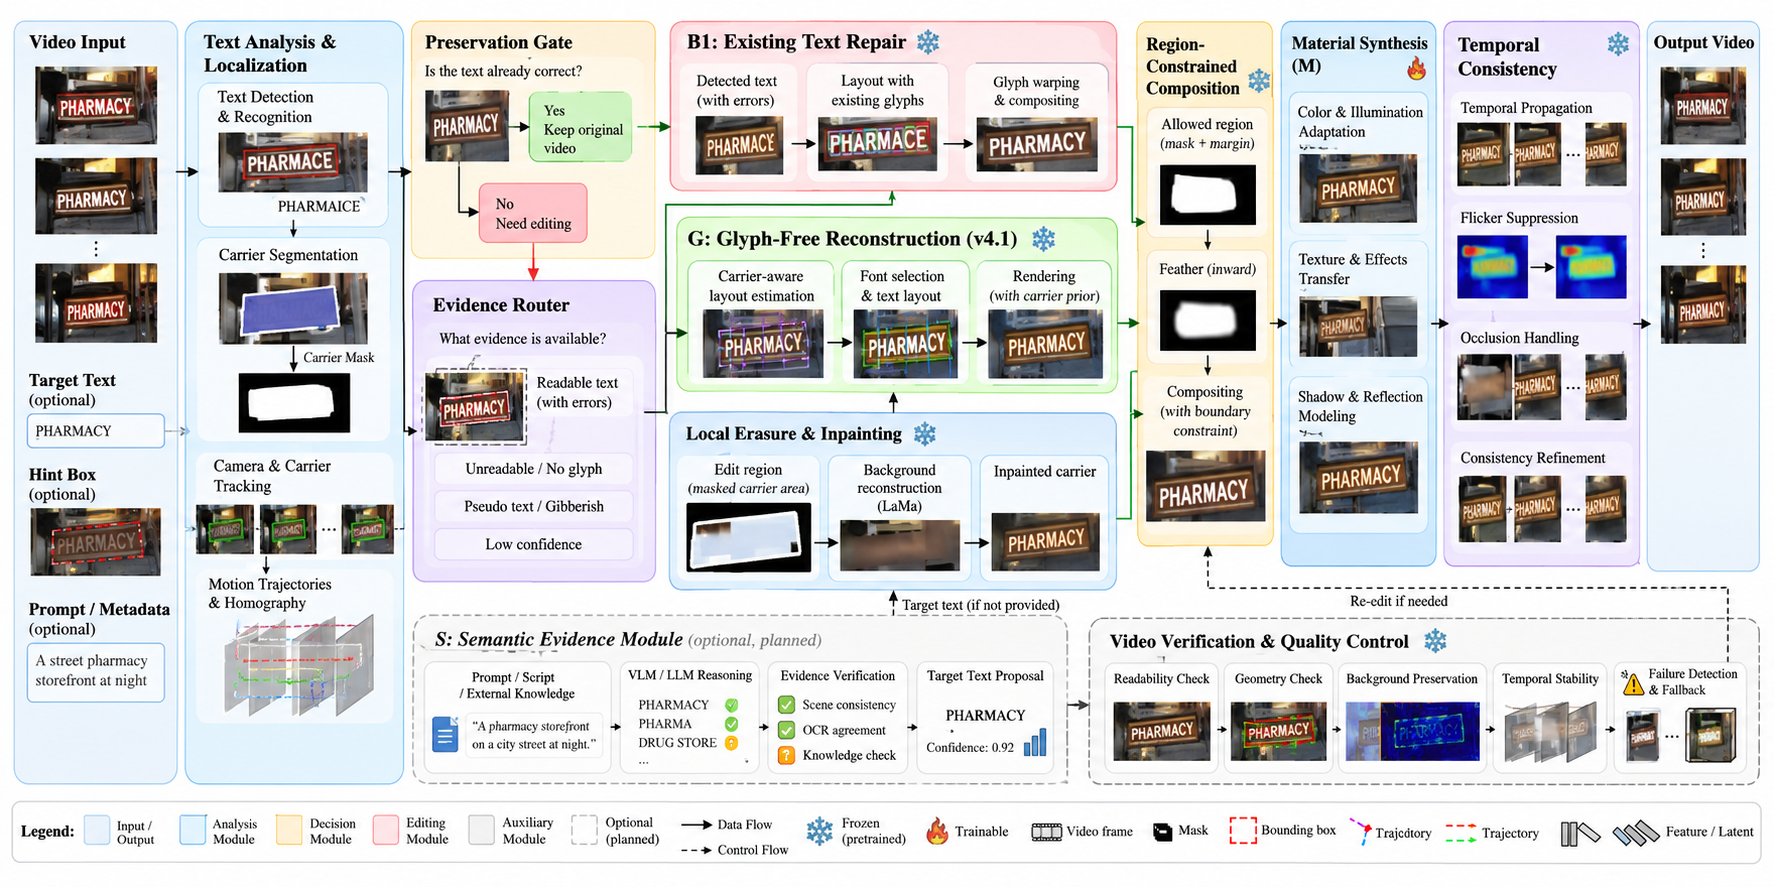
\includegraphics[width=\linewidth]{figs/fig_overview_framework.png}
\caption{\textbf{\method framework and the scope of this paper.} Text analysis reads and tracks the text and its carrier; the preservation gate returns the clip unchanged when the text already reads the target; otherwise the evidence available decides between repairing the existing text (B1) and glyph-free reconstruction (G); local erasure and a region-constrained compositor keep every edit inside the allowed region. \emph{Status:} all reported results come from the frozen B1 path; its only appearance step is the non-parametric source appearance transport, nothing is trained, and of the temporal box only carrier-anchored propagation belongs to it. G failed its sealed test and is exploratory (\cref{sec:exp_neg}). The appearance backend is an external model~\cite{zeng2026steervte} used only in Banksy-V (\cref{sec:exp_hybrid}); M, S, the router and the verification loop are planned, and a trained material generator was negative.}
\label{fig:overview}
\end{figure*}


\method takes a generated clip $V=\{I_t\}_{t=1}^{T}$, a target string $s$ and a hint box $b$ (\cref{sec:task}) and returns a clip $\hat V$ that differs from $V$ only inside the text region. \Cref{fig:overview} summarises the pipeline; all components are classical or pre-trained and nothing is trained for the task. We describe the steps in order and give thresholds and implementation details in the supplement.

\subsubsection{Reading the text and tracking its carrier}
\label{sec:read}
We run an off-the-shelf OCR system (EasyOCR~\cite{easyocr}, CRAFT detection~\cite{baek2019craft} and CRNN recognition~\cite{shi2017crnn}) on every frame and keep the boxes that overlap $b$. Boxes are grouped into text rows, and the frame whose rows best match $s$ (normalised edit similarity) becomes the reference frame $t^\star$. The text is printed on, or emitted by, a physical \emph{carrier}---a sign, a poster, a screen---so we track the carrier rather than the glyphs: SIFT keypoints~\cite{lowe2004sift} are matched between $I_{t^\star}$ and every $I_t$ inside a window one text-box size larger on each side of the reference quad, and a RANSAC~\cite{fischler1981ransac} homography $H_t$ is estimated (ratio test 0.75, reprojection threshold 2.5\,px, at least 10 inliers). When a frame fails, $H_t$ falls back to the quad-to-quad homography between the OCR boxes. Everything that is placed on the carrier later---erased background, glyphs, masks---is placed once in the reference frame and carried to frame $t$ by $H_t$, which removes per-frame jitter of the OCR boxes from the output.

\subsubsection{Preservation gate}
\label{sec:pres}
Generated text is often already correct, and any edit can only make such a clip worse. The preservation gate returns $\hat V=V$ when the OCR evidence across frames shows that the clip already reads $s$: the complete target is read in at least 85\% of the frames, wrong readings occur in at most 5\%, the reading lies inside the hint box, at most 10\% of the frames contain extra boxes, and the reading of all boxes inside the hint box, concatenated in reading order, equals $s$ in at least 90\% of the correct frames. The last condition prevents skipping when the target appears next to other, garbled text (\eg, a correct word above a garbled subtitle). The gate uses only the OCR of the pipeline, never the evaluation reader (\cref{sec:metrics}), and when the evidence is insufficient the clip is edited: the gate trades recall for safety. In the final run it skips \rSkipped{} of the 526 clips (9\%), all of which the independent reader confirms as correct.

\subsubsection{Localization gate and layout}
\label{sec:loc}
If the old glyphs can be localised reliably, the new text should inherit their size, colour and baseline. We estimate a glyph \emph{instance} in the reference frame: the ink mask (colour clustering inside the rows), the ink and ground colours, the letter height, the number of letters and the letter band. The localization gate accepts the instance only if it contains at least three letters (two for Chinese), the local contrast between ink and inter-letter ground exceeds 40 in CIELAB, the letter height is between 0.3 and 1.0 of the OCR box height, and the OCR rows did not require a fallback grouping. Otherwise the clip falls back to a \emph{box layout} that fills the tracked box with legible text. In the final run, \rBoxPolicy{} of the \rOursCollatN{} clips that \method edits (35\%) take the box layout.

With an accepted instance, the target is laid out on the letter band: the cap height equals the measured letter height, the string keeps its natural aspect ratio in the selected font, and it is centred on the old text; a target wider than the old line may extend the line by up to $1.35\times$ before its height is reduced. The band is oriented like the OCR quad, which for most detectors is axis-aligned---a limitation we return to in \cref{sec:limits}. Stacked text keeps its rows: the target is split into lines following the word counts of the detected rows, and each line is laid out on its own row instance.

\subsubsection{Erasure and deterministic rendering}
\label{sec:render}
\paragraph{Erasure.} The old glyphs are removed once, in the reference frame: the ink mask (closed, and extended by the bright pixels of glowing text) is dilated by $\min(0.3h,\max(10,0.18h))$ pixels for text height $h$, flat grounds are pre-filled with their median colour, and the hole is inpainted with LaMa~\cite{suvorov2022lama}. The erased background is then carried to every frame by $H_t$, with a per-frame, per-channel gain fitted on a ring around the hole and smoothed over five frames, so that exposure changes follow without per-frame inpainting flicker.

\paragraph{Font matching.} The new glyphs are rendered, not generated. The font is chosen from a library of 33 Latin and 8 Chinese families (variable fonts expanded over their weights) by comparing stroke statistics of the warped old ink mask with those of each candidate rendered in the same layout; script and display faces are admitted only when they are clearly better (distance below 0.6 of the best plain face). Because the target string is drawn by a font rasteriser, its spelling is exact by construction.

\paragraph{Photometry.} The glyph colour follows the per-frame ink colour of the old text (running median over seven frames) modulated by a low-frequency shading field estimated from the old strokes in canonical text coordinates, and glowing text receives a soft halo. The canvas is warped to every frame with $H_t$ and composited over the erased background.

\subsubsection{Appearance gate and source appearance transport}
\label{sec:sat}
Rendering gives the right letters, but on emissive carriers---neon, lightboxes, screens---the old glyphs carry glow, bloom and inner structure that a flat fill cannot reproduce. SAT transports this appearance from the old glyphs to the new ones without regenerating the region. Let $B$ be the erased background, $I$ the reference frame and $d(x)$ the signed distance of pixel $x$ to the boundary of the old glyphs, in units of the letter height. On the old text we fit, per distance bin $k$ and per channel, a multiplicative-plus-additive light-transport operator
\begin{equation}
I(x)\approx m_k\,B(x)+a_k,\qquad k=k(d(x)),
\label{eq:sat}
\end{equation}
over the support $d\le0.6$, and apply it to the new glyphs with their own distance field, $\hat I(x)=m_{k(\hat d(x))}B(x)+a_{k(\hat d(x))}$. On the old text, this family reconstructs the source better than an additive-only operator, a distance-indexed replacement or a flat fill (cross-validated CIELAB error 17.2 vs.\ 25.9, 27.6 and 29.7; best on 45 of 52 clips; supplement), which is why we keep both terms.

SAT is applied only behind an \emph{appearance gate} with two conditions: the text must be emissive (ink brighter than its ground, or a detected glow on the carrier), and the operator must generalise across the text---fitted on one half and tested on the other, in both directions, its error must stay below 0.75 of the flat-fill error. In the final run, SAT is enabled on \rSatOn{} clips (10\%); it is never applied to box-layout clips, whose instance evidence is weak by definition.

\subsubsection{Compositing}
The output differs from the input only where the erasure mask or the new glyphs (with halo) are non-zero; elsewhere the input pixels are copied, so the only residual outside the text region is the re-encoding of the video.

\subsection{Benchmark details}
\label{sec:supp_bench}

\paragraph{Generation.} Clips were generated with the text-to-video mode of VACE-14B from 120 prompts, each asking for a scene with a sign of a given material that reads a quoted target string, with ten seeds per prompt; 1{,}178 of the 1{,}200 generations were usable (832$\times$464, 49 frames, 15\,fps). An OCR screen confirmed the requested text in 24\% of them (English 21\%, Chinese 27\%). The screen reads every fourth frame with EasyOCR and takes, per frame, the best normalised edit similarity between a recognised string and the target; a clip counts as correct when at least 80\% of these frames reach 0.8. The 526 benchmark clips are exactly the clips that fail this test but have a mean similarity of at least 0.3, i.e.\ contain a recognisable attempt at the target; the other 371 were dropped; our evaluation reader judges \rOrigRead\% of them correct (\cref{tab:main}), so the benchmark contains repair and do-nothing cases.

\paragraph{Targets and composition.} The 40 target strings are: \str{BUS STOP} (25 clips), \str{FRESH BREAD} (23), \str{BOOK STORE} (22), \str{PHARMACY} (22), \str{COFFEE SHOP} (21), \str{TEA HOUSE} (20), \str{NO PARKING} (19), \str{FLOWER MARKET} (19), \str{SALE 50\%} (18), \str{NIGHT MARKET} (18), \zh{面包房} (17), \zh{小心地滑} (17), \zh{邮局} (16), \str{ICE CREAM} (15), \zh{停车场} (15), \zh{电影院} (15), \zh{书店} (14), \str{RECORDS} (13), \zh{出口} (13), \zh{洗衣店} (13), \zh{咖啡店} (12), \zh{茶馆} (12), \zh{欢迎光临} (11), \zh{营业中} (11), \str{OPEN} (10), \str{EXIT} (10), \zh{理发店} (10), \str{GALLERY} (9), \zh{花店} (9), \zh{公园} (9), \zh{火锅} (9), \str{BAKERY} (8), \zh{夜市} (8), \str{HOTEL} (7), \zh{便利店} (7), \zh{药房} (7), \str{LAUNDRY} (6), \zh{水果店} (6), \str{CINEMA} (5) and \str{WELCOME} (5). \Cref{tab:supp_comp} gives the material $\times$ language composition and the readability of each method per group.

% generated by paper_numbers.py from r1full
\begin{table}[h]
\centering
\caption{Composition of the benchmark and readability (\%) per group (same run as \cref{tab:main}).}
\label{tab:supp_comp}
\small\setlength{\tabcolsep}{3pt}
\begin{tabular}{@{}lccccc@{}}
\toprule
Group & EN & ZH & Original & \steer & \method \\
\midrule
neon & 47 & 46 & 58.1 & 89.2 & 97.8 \\
signboard & 74 & 12 & 64.0 & 77.9 & 93.0 \\
wood & 20 & 34 & 63.0 & 90.7 & 92.6 \\
metal & 22 & 34 & 71.4 & 94.6 & 96.4 \\
glass & 52 & 24 & 34.2 & 77.6 & 84.2 \\
paper & 55 & 41 & 47.9 & 80.2 & 87.5 \\
screen & 25 & 40 & 43.1 & 83.1 & 89.2 \\
\midrule
English (295) & & & 62.0 & 84.1 & 91.5 \\
Chinese (231) & & & 43.3 & 84.0 & 91.3 \\
\bottomrule
\end{tabular}
\end{table}


\paragraph{Development data.} We disclose every clip that was inspected during development. (i) Twelve clips (``dev12'') were used to tune the instance front end and the SAT oracle; 24 random clips (``held24'') were not used for tuning, but screenshots of four of them were viewed during diagnosis and held24 informed the SAT margin, so they are not strictly held out. (ii) The 53 SAT-enabled clips were used for the SAT human study and then for the failure diagnosis of \cref{sec:exp_sat}; results of the padded canvas on them are development results. (iii) Forty clips were inspected while developing the selective-editing components; these are the clips excluded in the lower block of \cref{tab:main} and the right block of \cref{tab:selective}:
{\scriptsize\texttt{g001\_en\_neon\_s1 g006\_en\_paper\_s3 g007\_en\_glass\_s6 g008\_en\_signboard\_s0 g010\_en\_neon\_s9 g011\_en\_wood\_s1 g020\_en\_glass\_s5 g020\_en\_glass\_s7 g022\_en\_neon\_s1 g024\_en\_metal\_s0 g025\_en\_paper\_s4 g028\_en\_signboard\_s3 g029\_en\_screen\_s2 g036\_en\_neon\_s6 g045\_en\_signboard\_s8 g046\_en\_neon\_s2 g046\_en\_neon\_s4 g046\_en\_neon\_s5 g049\_en\_wood\_s5 g052\_en\_screen\_s4 g057\_en\_neon\_s6 g057\_en\_neon\_s7 g059\_en\_metal\_s2 g067\_zh\_wood\_s9 g071\_zh\_neon\_s0 g076\_zh\_neon\_s5 g076\_zh\_neon\_s8 g083\_zh\_neon\_s1 g084\_zh\_neon\_s0 g084\_zh\_neon\_s3 g093\_zh\_neon\_s7 g098\_zh\_neon\_s1 g107\_zh\_neon\_s2 g107\_zh\_neon\_s9 g110\_zh\_neon\_s0 g110\_zh\_neon\_s4 g110\_zh\_neon\_s5 g110\_zh\_neon\_s7 g110\_zh\_neon\_s8 g116\_zh\_screen\_s8}.} The main conclusions do not change when they are removed. (iv) Nine clips were inspected while developing source-glyph reuse (\cref{sec:exp_neg}): three development clips ({\scriptsize\texttt{g026\_en\_signboard\_s7 g055\_en\_signboard\_s6 g024\_en\_metal\_s2}}) and six clips of the originally registered 30-clip evaluation sample that were viewed while debugging and therefore moved to the development set ({\scriptsize\texttt{g008\_en\_signboard\_s8 g025\_en\_paper\_s7 g026\_en\_signboard\_s0 g029\_en\_screen\_s6 g035\_en\_glass\_s8 g054\_en\_glass\_s0}}). \Cref{tab:reuse} excludes both (iii) and (iv).

\subsection{Evaluation details}
\label{sec:supp_eval}

\paragraph{Reader.} Qwen2.5-VL-7B transcribes the hint-box crop (15\% padding) of frames 0, 12, 24, 36 and 48. A frame is exact if its normalised edit similarity to the target is at least 0.999 after normalisation (whitespace removed, lower-cased, traditional Chinese folded to simplified); a clip is correct if at least 4 of 5 frames are exact. An earlier draft of the pre-registration described this as ``at least 60\% of frames''; this was a documentation error, the code was fixed before the run, and the decisions are unaffected.

\paragraph{Evaluation hygiene.} In an earlier phase, the reader produced garbled transcriptions (a repeated token) for about 8.5\% of the inputs on one cluster (x86, an older version of the inference library) and none on another (aarch64, newer version). Two refiners had been read on the clean system and their baselines on the faulty one, which inflated a comparison by 16.6 points; after re-reading everything in one job the advantage disappeared (\cref{sec:supp_refiner}). Since then, every table is produced by re-reading all of its rows in a single job, and we check transcriptions for garbage. Re-reading identical outputs in a second job changes readability by about one point, which is why we treat differences of that size as ties: when the 99 unchanged originals of the two-row re-run were read again, 75 received identical transcriptions and 98 the same verdict. The front end itself is not bit-reproducible across runs (GPU OCR boxes, LaMa on different devices); comparing two passes of identical code gives no significant difference in appearance or flicker but a 0.46\,dB difference in background PSNR, so we only compare variants from the same pass.

\paragraph{Appearance distance.} Features per frame (CIELAB, inside the box): ink colour difference to the original, ink--ground contrast difference, halo excess normalised by contrast, boundary gradient normalised by contrast (edge softness), and standard deviation of lightness inside the eroded strokes (inner shading). The original compared with itself scores about 0.27, the estimation floor. Each feature is divided by its median over all method--clip pairs of the run, so values are comparable only within one evaluation job. The ink segmentation inside the estimator uses $k$-means with random initialisation (OpenCV's $k$-means++ without a fixed seed), so scores are not bit-reproducible: in the run of \cref{tab:main}, \rRetestN{} clips were scored twice on byte-identical outputs (B1 and R1 where reuse did not apply), and the two scores agreed exactly in \rRetestSame{} clips, with a per-clip standard deviation of the difference of \rRetestSD{} and a mean difference of $\rRetestMean$ [$\rRetestLo$, $\rRetestHi$] (the pair B1f/R1f: $\rRetestMeanB$). The evaluation code is frozen, so we report this noise instead of changing the estimator; differences of a few hundredths in a run mean are within it.

\subsection{Implementation details}
\label{sec:supp_impl}

\paragraph{Reference frame.} Among the frames whose OCR score is at least 90\% of the maximum, the one closest to the middle of the clip.

\paragraph{Gates.} Preservation gate: complete target read in $\geq$85\% of the frames, wrong readings in $\leq$5\%, reading inside the hint box, extra boxes in $\leq$10\% of the frames, and the concatenated reading of all boxes inside the hint box equal to the target in $\geq$90\% of the correct frames. Localization gate: $\geq$3 letters ($\geq$2 for Chinese), CIELAB distance between ink inside the letter band and inter-letter ground $\geq$40, letter height between 0.3 and 1.0 of the OCR box height, no fallback row grouping; otherwise the box policy is used (\rBoxPolicy{} of the \rOursCollatN{} clips that \method edits in the final run, most often because OCR grouped the text into rows that the instance estimate could not confirm; in an earlier pass, the reasons were the row grouping for 134, letter height for 67, letter count for 40 and contrast for 36 clips, with overlaps). Appearance gate: emissive text (ink brighter than ground, or glow detected on the carrier) and a cross-validated error ratio below 0.75 against the flat fill in both directions.

\paragraph{Letter height and polarity.} Latin letter height is the median height of letter-like components (solidity $\geq$0.85); Chinese letter height is taken from the ink distribution. Ink and ground are separated by $k$-means with $k\in\{2,3\}$ scored by letter morphology (component heights and holes), with a fixed seed.

\paragraph{Font library.} 33 Latin and 8 Chinese families from Google Fonts, variable fonts expanded over their weights. In the final run, \rLatinFam{} Latin families and \rZhFam{} Chinese families were selected (Noto Sans SC for \rNotoPct\% of the edited Chinese clips, Noto Serif SC for \rNotoSerifPct\%, ZCOOL XiaoWei for \rZcoolPct\%).

\paragraph{SAT.} The operator of \cref{eq:sat} is fitted per distance bin (signed distance in letter heights, support up to 0.6 outside the strokes) by least squares on the reference frame and applied to every frame through the carrier homography. The flat fill is the ink colour of the box policy. Cross-validation fits on the left half of the text row and tests on the right half, and vice versa.

\paragraph{Runtime.} On an NVIDIA A40, the earlier front end took about 20\,s per clip and the learned refiner about 40\,s per clip; \steer reports 108\,s per 49-frame clip on its hardware. In a controlled measurement of the frozen final pipeline on 60 benchmark clips drawn at random (one process on one NVIDIA V100S with 32\,GB and 9 CPU cores, the final run's flags, a fresh output folder so that nothing is served from a cache, models loaded once), a clip took 18.2\,s on average (median 18.0\,s; 10th to 90th percentile 15.8 to 20.6\,s; range 13.5 to 22.6\,s), and loading the models plus one warm-up clip took 44.7\,s. The three sampled clips that the preservation gate left unchanged still took 15.2 to 17.3\,s, because the gate reads every frame. On GH200 nodes the 100 VTE-Bench clips took about 8.6\,s per clip and GPU (two parallel workers, 7\,min 11\,s after a model-loading time of 28\,s), a wall-clock estimate from the run logs.


% Scope and roadmap (route A, 2026-10-28): the framework figure moved here from the main paper.
\paragraph{Scope and roadmap.} \Cref{fig:roadmap} places the evaluated pipeline in the broader framework we are working towards. Only the B1 path is evaluated in this paper; the figure is a roadmap and states the status of every other box.
% Research roadmap (the user's framework raster, relabelled 2026-10-27 by figs/src/relabel_framework.py). Supplement only, not the method figure.
\begin{figure*}[t]
\centering
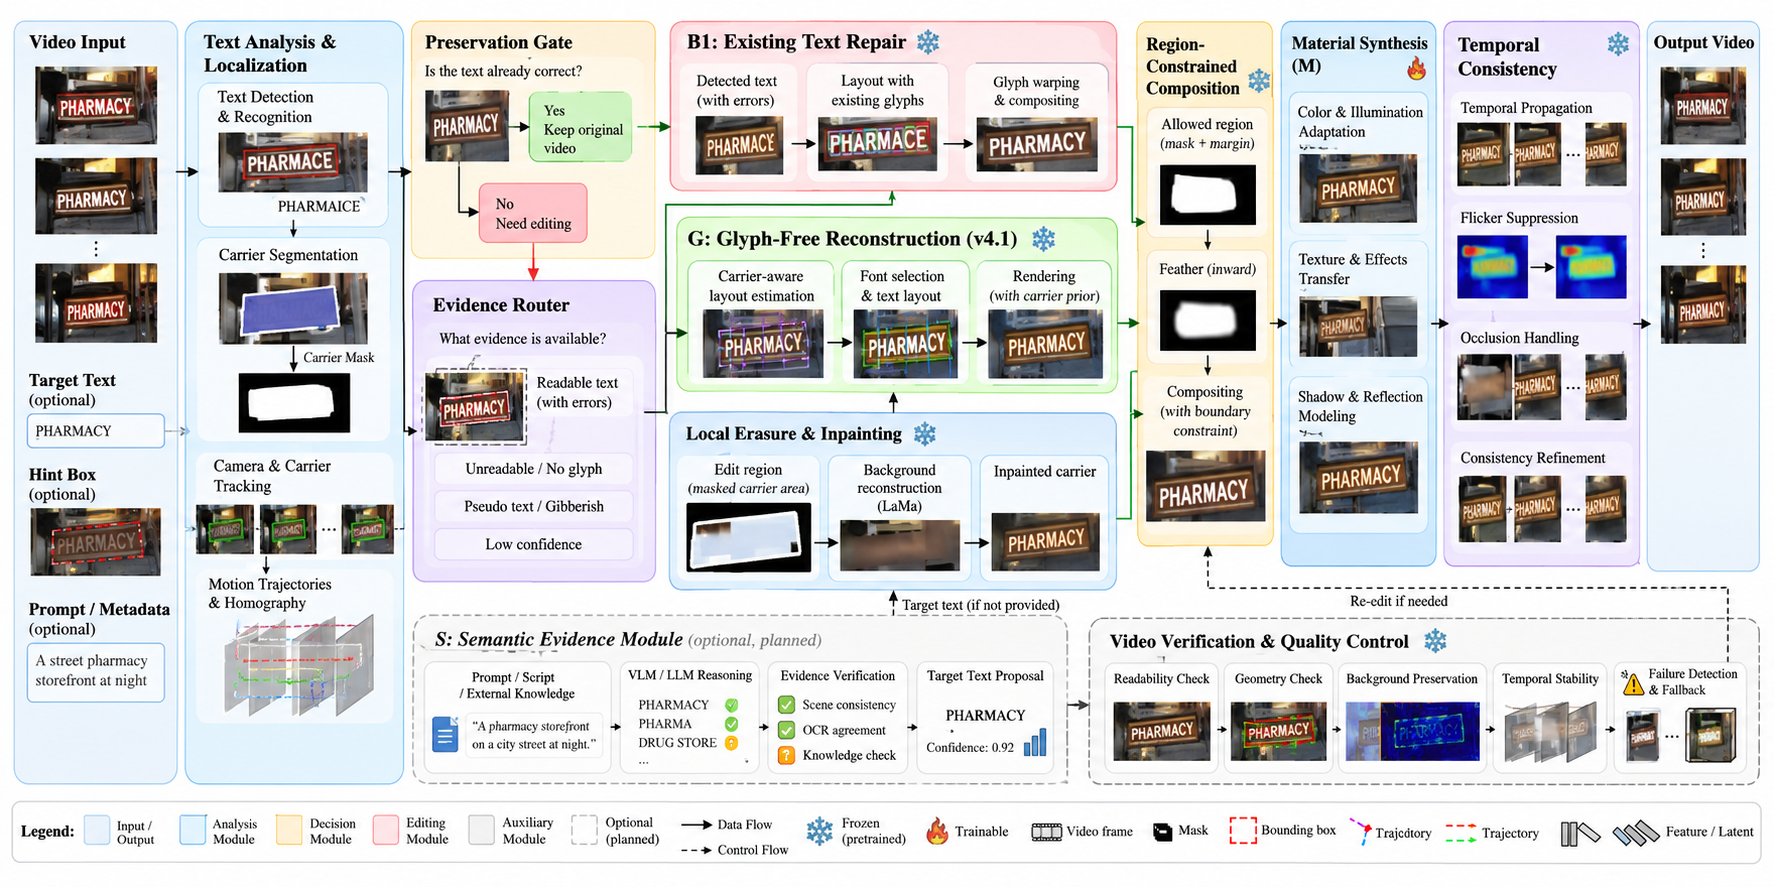
\includegraphics[width=\linewidth]{figs/fig_overview_framework.png}
\caption{\textbf{Research roadmap, not the evaluated method.} The broader framework this work belongs to. Text analysis, the preservation gate, B1 and the region-constrained compositor form the pipeline evaluated in this paper. G, the glyph-free branch, did not pass its sealed cross-generator test and is an exploratory extension (\cref{sec:supp_l3}). The appearance backend is an external pretrained model~\cite{zeng2026steervte}, used only in the Banksy-V hybrid; the constrained fusion (M), the semantic evidence module (S), the evidence router and the verification loop are planned and not claimed, and a trained material generator was a negative result (\cref{sec:exp_neg}). Of the temporal box, only carrier-anchored propagation is part of B1.}
\label{fig:roadmap}
\end{figure*}



\section{Complete experimental sections}
\label{sec:supp_exp}
\subsubsection{Main results in full}
\label{sec:exp_full}

\paragraph{Protocol.} \Cref{tab:main}, \cref{tab:reuse} and every number in \cref{sec:main,sec:exp_local,sec:exp_neg} come from one front-end pass over the 526 benchmark clips with the final system and the variants of \cref{sec:exp_neg}, which share the OCR, tracking and instance estimation and are therefore paired clip by clip; these outputs, the original clips and \steer's outputs were read by the same reader in one evaluation job (\cref{sec:metrics}). Every other table comes from its own front-end pass and its own evaluation run, named in its caption (\cref{tab:selective,tab:external,tab:readers} were evaluated on a second machine whose decoded crops are byte-identical to the first; supplement); because the appearance distance is normalised within each run, it is compared only within a table. Paired differences are reported with 95\% bootstrap confidence intervals over clips~\cite{efron1994bootstrap} (10{,}000 resamples) and readability differences with exact McNemar tests~\cite{mcnemar1947}. Forty clips were inspected while developing the selective-editing components (\cref{sec:exp_sel}); \cref{tab:main} reports all clips and, separately, the 486 clips that were never inspected.

\paragraph{Baseline.} \steer~\cite{zeng2026steervte} is the strongest published video text editor; it adds glyph and style conditioning to a frozen VACE-14B backbone~\cite{jiang2025vace} and is trained on one million triplets. We ran the released model on every clip with the hint box as editing mask and the target as text, at the same resolution and length as the input. Its outputs are generated end to end, so they are evaluated as they are.

% generated by paper_numbers.py: Table 1 from r1full (one front-end pass, one evaluation job)
\begin{table*}[t]
\centering
\caption{\textbf{Main results} (526 clips; one front-end pass and one evaluation job for every row). Readability: share of clips whose text the reader transcribes exactly in at least 4 of 5 frames. Fixed / broken: garbled $\to$ correct and correct $\to$ wrong transitions relative to the original as read in the same job; net = fixed $-$ broken. Appearance: glyph-agnostic material distance to the original text (normalised within this run; lower is closer). BG PSNR: outside the dilated text region. Flicker and jitter: motion-compensated, inside the text box (grey levels). The lower block excludes the 40 clips inspected while developing the selective-editing components.}
\label{tab:main}
\setlength{\tabcolsep}{4.5pt}
\resizebox{\linewidth}{!}{%
\begin{tabular}{@{}lccccccccc@{}}
\toprule
 & Readability $\uparrow$ & Fixed $\uparrow$ & Broken $\downarrow$ & Net $\uparrow$ & NED sim.\ $\uparrow$ & Appearance $\downarrow$ & BG PSNR $\uparrow$ & Flicker $\downarrow$ & Jitter $\downarrow$ \\
\midrule
\multicolumn{10}{@{}l}{\emph{All 526 clips}} \\
Original (generated) & 53.8 & -- & -- & -- & 0.820 & -- & -- & 1.98 & 9.18 \\
\steer~\cite{zeng2026steervte} & 84.0 & 165 & \textbf{6} & 159 & 0.946 & \textbf{1.83} & 36.49 & \textbf{1.66} & 8.30 \\
\method & \textbf{91.4} & \textbf{210} & 12 & \textbf{198} & \textbf{0.959} & 2.57 & \textbf{42.52} & 1.79 & \textbf{7.86} \\
\midrule
\multicolumn{10}{@{}l}{\emph{486 clips outside the development set}} \\
Original (generated) & 54.7 & -- & -- & -- & 0.822 & -- & -- & 1.97 & 9.12 \\
\steer~\cite{zeng2026steervte} & 84.4 & 150 & \textbf{6} & 144 & 0.945 & \textbf{1.85} & 36.40 & \textbf{1.65} & 8.24 \\
\method & \textbf{91.2} & \textbf{189} & 12 & \textbf{177} & \textbf{0.958} & 2.60 & \textbf{42.50} & 1.79 & \textbf{7.86} \\
\bottomrule
\end{tabular}}
\end{table*}


\paragraph{Main comparison.}
\label{sec:main}
\Cref{tab:main} compares \method with \steer and with the unedited clips. \method makes \rOursRead\% of the clips readable, \rReadGain{} points more than \steer (\rOnlyOurs{} clips are correct only with \method, \rOnlySteer{} only with \steer; McNemar $p=\rMcNemarP$), and turns \rOursFixed{} of the \rGarbled{} garbled clips into correct ones. It is not free of damage: it breaks \rOursBroken{} of the \rOrigCorrect{} originally correct clips where \steer breaks \rSteerBroken, so its advantage in net repairs (\rOursNet{} vs.\ \rSteerNet) is smaller than in repairs alone. The picture is unchanged on the 486 clips outside the development set (\rOursReadND\% vs.\ \rSteerReadND\%; \rOursNetND{} vs.\ \rSteerNetND{} net repairs).

The two methods trade different qualities. \method leaves the background intact---its PSNR outside the text region is \rBGDiff\,dB higher (95\% CI [\rBGDiffLo, \rBGDiffHi]; higher on \rBGHigherPct\% of the clips)---and its strokes jitter less (edge jitter \rOursJitter{} vs.\ \rSteerJitter), because every glyph is placed once on the tracked carrier. \steer's text region flickers less (\rSteerFlicker{} vs.\ \rOursFlicker) and, above all, its text looks more like the original: its appearance distance is \rSteerMad{} against \rOursMad{} for \method. We analyse this gap in \cref{sec:limits}.

\Cref{fig:material} breaks readability down by carrier material. \method is ahead of \steer on all seven materials; the largest gains are on signboards (+\rGainSignboard{} points) and neon (+\rGainNeon), where \steer most often keeps the garbled characters, and the smallest on metal (+\rGainMetal) and wood (+\rGainWood). By language, \method reaches \rOursEn\% on the \rEnN{} English and \rOursZh\% on the \rZhN{} Chinese clips (\steer: \rSteerEn\% and \rSteerZh\%). \Cref{fig:qual} shows randomly sampled examples, including two failures of \method (\zh{公园} on neon, \zh{花店} on glass); \cref{fig:wins} shows selected clips that only \method repairs, a case about five times as frequent as the reverse (41 vs.\ 8 clips outside the development set under both readers).

% generated by analyze_judge2.py
\begin{table}[t]
\centering
\caption{\textbf{Readability under different readers} (the outputs of \cref{tab:main}; identical crops, frames, prompt, decoding and scoring). W/L: clips correct only with \method / only with \steer, with the exact McNemar $p$. Agree: share of clip--method verdicts equal to the first reader's (\cref{tab:main}). The re-read uses the first reader on the second readers' hardware.}
\label{tab:readers}
\setlength{\tabcolsep}{2.5pt}
\resizebox{\linewidth}{!}{%
\begin{tabular}{@{}lcccccc@{}}
\toprule
Reader & $n$ & Original & \steer & \method & W/L ($p$) & Agree \\
\midrule
Qwen2.5-VL-7B (A40; \cref{tab:main}) & 526 & 53.8 & 84.0 & 91.4 & 70/31 ($1.3\times10^{-4}$) & -- \\
Qwen2.5-VL-7B, re-read (V100) & 526 & 53.8 & 84.0 & 91.8 & 70/29 ($4.6\times10^{-5}$) & 99.9 \\
InternVL2.5-8B (V100) & 526 & 49.6 & 78.7 & 84.8 & 74/42 ($3.8\times10^{-3}$) & 91.1 \\
Pixtral-12B, English only (V100) & 295 & 60.0 & 80.3 & 77.6 & 27/35 ($0.37$) & 88.2 \\
Qwen2.5-VL-7B (A40), English only & 295 & 62.0 & 84.1 & 91.5 & 40/18 ($5.4\times10^{-3}$) & -- \\
\bottomrule
\end{tabular}}
\end{table}

\paragraph{A second reader.} Readability depends on the reader, so we registered a re-reading of the outputs of \cref{tab:main} by readers from other model families, with identical crops, frames, prompt, decoding and scoring, and a decision rule fixed in advance: the advantage counts as reader-robust only if the main second reader, InternVL2.5-8B (InternViT vision encoder, InternLM2.5 language model), finds \method more readable than \steer with $p<0.05$ (\cref{tab:readers}). It does: \jIvlOurs\% against \jIvlSteer\% (\jIvlOnlyOurs{} vs.\ \jIvlOnlySteer{} discordant clips, McNemar $p=\jIvlP$; \jIvlOursNet{} vs.\ \jIvlSteerNet{} net repairs), although the margin is smaller than under the first reader and, split by language, significant only for Chinese (\jIvlZhOurs\% vs.\ \jIvlZhSteer\%, $p=\jIvlZhP$; English \jIvlEnOurs\% vs.\ \jIvlEnSteer\%, $p=\jIvlEnP$). InternVL is stricter with every method and agrees with the first reader on about 91\% of the clip--method verdicts. A third reader, Pixtral-12B, cannot read Chinese---it invents unrelated text on every Chinese crop---and was registered for the 295 English clips only; there it finds no advantage (\jPixOurs\% vs.\ \jPixSteer\%, $p=\jPixP$). Most of its errors on \method's outputs are correct transcriptions followed by invented text (\jPixExtraOurs\% of the frames, against \jPixExtraSteer\% for \steer), which exact matching counts as wrong; when a frame only has to contain the target (an exploratory criterion defined after the reads), Pixtral finds the two methods level (\jPixContOurs\% vs.\ \jPixContSteer\%). The second readers ran on different GPUs from the first reader, with byte-identical crops; the first reader re-reading the outputs on those GPUs reproduces \jQrAgreeOurs--100\% of its verdicts per method, so the hardware does not explain these differences.

\begin{figure}[t]
\centering
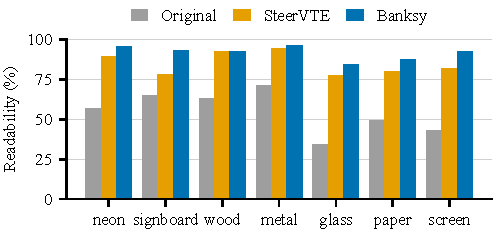
\includegraphics[width=\linewidth]{figs/plots/material_readability.pdf}
\caption{\textbf{Readability by carrier material} (all 526 clips; 54 to 96 clips per material).}
\label{fig:material}
\end{figure}

\begin{figure*}[t]
\centering
\setlength{\tabcolsep}{1.2pt}\renewcommand{\arraystretch}{0.6}
\begin{tabular}{@{}m{0.95cm}cccccc@{}}
&\footnotesize\textbf{Original} & \footnotesize\textbf{SteerVTE} & \footnotesize\textbf{Banksy} & \footnotesize\textbf{Original} & \footnotesize\textbf{SteerVTE} & \footnotesize\textbf{Banksy} \\[2pt]
\scriptsize neon & 
\includegraphics[width=0.146\linewidth]{figs/cells/qual_g001_en_neon_s2_orig.jpg} & 
\includegraphics[width=0.146\linewidth]{figs/cells/qual_g001_en_neon_s2_steervte.jpg} & 
\includegraphics[width=0.146\linewidth]{figs/cells/qual_g001_en_neon_s2_B1.jpg} & 
\includegraphics[width=0.146\linewidth]{figs/cells/qual_g100_zh_neon_s5_orig.jpg} & 
\includegraphics[width=0.146\linewidth]{figs/cells/qual_g100_zh_neon_s5_steervte.jpg} & 
\includegraphics[width=0.146\linewidth]{figs/cells/qual_g100_zh_neon_s5_B1.jpg} \\
&\parbox[t]{0.146\linewidth}{\centering\scriptsize \textcolor{badred}{\ding{55}}\,\texttt{OFFEE SHOP}} & \parbox[t]{0.146\linewidth}{\centering\scriptsize \textcolor{okgreen}{\ding{51}}\,\texttt{COFFEE SHOP}} & \parbox[t]{0.146\linewidth}{\centering\scriptsize \textcolor{okgreen}{\ding{51}}\,\texttt{COFFEE SHOP}} & \parbox[t]{0.146\linewidth}{\centering\scriptsize \textcolor{badred}{\ding{55}}\,\texttt{\zh{公公}}} & \parbox[t]{0.146\linewidth}{\centering\scriptsize \textcolor{okgreen}{\ding{51}}\,\texttt{\zh{公园}}} & \parbox[t]{0.146\linewidth}{\centering\scriptsize \textcolor{badred}{\ding{55}}\,\texttt{\zh{公园}}} \\[3pt]
\scriptsize signboard & 
\includegraphics[width=0.146\linewidth]{figs/cells/qual_g008_en_signboard_s4_orig.jpg} & 
\includegraphics[width=0.146\linewidth]{figs/cells/qual_g008_en_signboard_s4_steervte.jpg} & 
\includegraphics[width=0.146\linewidth]{figs/cells/qual_g008_en_signboard_s4_B1.jpg} & 
\includegraphics[width=0.146\linewidth]{figs/cells/qual_g085_zh_signboard_s8_orig.jpg} & 
\includegraphics[width=0.146\linewidth]{figs/cells/qual_g085_zh_signboard_s8_steervte.jpg} & 
\includegraphics[width=0.146\linewidth]{figs/cells/qual_g085_zh_signboard_s8_B1.jpg} \\
&\parbox[t]{0.146\linewidth}{\centering\scriptsize \textcolor{badred}{\ding{55}}\,\texttt{FRESY BREAD}} & \parbox[t]{0.146\linewidth}{\centering\scriptsize \textcolor{badred}{\ding{55}}\,\texttt{FRESY BREAD}} & \parbox[t]{0.146\linewidth}{\centering\scriptsize \textcolor{okgreen}{\ding{51}}\,\texttt{FRESH BREAD}} & \parbox[t]{0.146\linewidth}{\centering\scriptsize \textcolor{badred}{\ding{55}}\,\texttt{\zh{夜市} Qingdao Night Marke}} & \parbox[t]{0.146\linewidth}{\centering\scriptsize \textcolor{okgreen}{\ding{51}}\,\texttt{\zh{夜市}}} & \parbox[t]{0.146\linewidth}{\centering\scriptsize \textcolor{okgreen}{\ding{51}}\,\texttt{\zh{夜市}}} \\[3pt]
\scriptsize wood & 
\includegraphics[width=0.146\linewidth]{figs/cells/qual_g014_en_wood_s6_orig.jpg} & 
\includegraphics[width=0.146\linewidth]{figs/cells/qual_g014_en_wood_s6_steervte.jpg} & 
\includegraphics[width=0.146\linewidth]{figs/cells/qual_g014_en_wood_s6_B1.jpg} & 
\includegraphics[width=0.146\linewidth]{figs/cells/qual_g105_zh_wood_s1_orig.jpg} & 
\includegraphics[width=0.146\linewidth]{figs/cells/qual_g105_zh_wood_s1_steervte.jpg} & 
\includegraphics[width=0.146\linewidth]{figs/cells/qual_g105_zh_wood_s1_B1.jpg} \\
&\parbox[t]{0.146\linewidth}{\centering\scriptsize \textcolor{badred}{\ding{55}}\,\texttt{TEXOITYIO}} & \parbox[t]{0.146\linewidth}{\centering\scriptsize \textcolor{okgreen}{\ding{51}}\,\texttt{EXIT}} & \parbox[t]{0.146\linewidth}{\centering\scriptsize \textcolor{okgreen}{\ding{51}}\,\texttt{EXIT}} & \parbox[t]{0.146\linewidth}{\centering\scriptsize \textcolor{badred}{\ding{55}}\,\texttt{\zh{小悒念滑}}} & \parbox[t]{0.146\linewidth}{\centering\scriptsize \textcolor{okgreen}{\ding{51}}\,\texttt{\zh{小心地滑}}} & \parbox[t]{0.146\linewidth}{\centering\scriptsize \textcolor{okgreen}{\ding{51}}\,\texttt{\zh{小心地滑}}} \\[3pt]
\scriptsize metal & 
\includegraphics[width=0.146\linewidth]{figs/cells/qual_g024_en_metal_s2_orig.jpg} & 
\includegraphics[width=0.146\linewidth]{figs/cells/qual_g024_en_metal_s2_steervte.jpg} & 
\includegraphics[width=0.146\linewidth]{figs/cells/qual_g024_en_metal_s2_B1.jpg} & 
\includegraphics[width=0.146\linewidth]{figs/cells/qual_g089_zh_metal_s3_orig.jpg} & 
\includegraphics[width=0.146\linewidth]{figs/cells/qual_g089_zh_metal_s3_steervte.jpg} & 
\includegraphics[width=0.146\linewidth]{figs/cells/qual_g089_zh_metal_s3_B1.jpg} \\
&\parbox[t]{0.146\linewidth}{\centering\scriptsize \textcolor{badred}{\ding{55}}\,\texttt{PHARMAICE}} & \parbox[t]{0.146\linewidth}{\centering\scriptsize \textcolor{okgreen}{\ding{51}}\,\texttt{PHARMACY}} & \parbox[t]{0.146\linewidth}{\centering\scriptsize \textcolor{okgreen}{\ding{51}}\,\texttt{PHARMACY}} & \parbox[t]{0.146\linewidth}{\centering\scriptsize \textcolor{badred}{\ding{55}}\,\texttt{\zh{澎影院}}} & \parbox[t]{0.146\linewidth}{\centering\scriptsize \textcolor{badred}{\ding{55}}\,\texttt{\zh{洹影院}}} & \parbox[t]{0.146\linewidth}{\centering\scriptsize \textcolor{okgreen}{\ding{51}}\,\texttt{\zh{电影院}}} \\[3pt]
\scriptsize glass & 
\includegraphics[width=0.146\linewidth]{figs/cells/qual_g007_en_glass_s2_orig.jpg} & 
\includegraphics[width=0.146\linewidth]{figs/cells/qual_g007_en_glass_s2_steervte.jpg} & 
\includegraphics[width=0.146\linewidth]{figs/cells/qual_g007_en_glass_s2_B1.jpg} & 
\includegraphics[width=0.146\linewidth]{figs/cells/qual_g090_zh_glass_s7_orig.jpg} & 
\includegraphics[width=0.146\linewidth]{figs/cells/qual_g090_zh_glass_s7_steervte.jpg} & 
\includegraphics[width=0.146\linewidth]{figs/cells/qual_g090_zh_glass_s7_B1.jpg} \\
&\parbox[t]{0.146\linewidth}{\centering\scriptsize \textcolor{badred}{\ding{55}}\,\texttt{FREST BREAD}} & \parbox[t]{0.146\linewidth}{\centering\scriptsize \textcolor{badred}{\ding{55}}\,\texttt{FRESB BREAD}} & \parbox[t]{0.146\linewidth}{\centering\scriptsize \textcolor{okgreen}{\ding{51}}\,\texttt{FRESH BREAD}} & \parbox[t]{0.146\linewidth}{\centering\scriptsize \textcolor{badred}{\ding{55}}\,\texttt{\cjkimg{cjk_b7d9d7d024} HUAJANGDIAN}} & \parbox[t]{0.146\linewidth}{\centering\scriptsize \textcolor{okgreen}{\ding{51}}\,\texttt{\zh{花店}}} & \parbox[t]{0.146\linewidth}{\centering\scriptsize \textcolor{badred}{\ding{55}}\,\texttt{\zh{南湖公园}}} \\[3pt]
\scriptsize paper & 
\includegraphics[width=0.146\linewidth]{figs/cells/qual_g034_en_paper_s3_orig.jpg} & 
\includegraphics[width=0.146\linewidth]{figs/cells/qual_g034_en_paper_s3_steervte.jpg} & 
\includegraphics[width=0.146\linewidth]{figs/cells/qual_g034_en_paper_s3_B1.jpg} & 
\includegraphics[width=0.146\linewidth]{figs/cells/qual_g096_zh_paper_s0_orig.jpg} & 
\includegraphics[width=0.146\linewidth]{figs/cells/qual_g096_zh_paper_s0_steervte.jpg} & 
\includegraphics[width=0.146\linewidth]{figs/cells/qual_g096_zh_paper_s0_B1.jpg} \\
&\parbox[t]{0.146\linewidth}{\centering\scriptsize \textcolor{badred}{\ding{55}}\,\texttt{SALE}} & \parbox[t]{0.146\linewidth}{\centering\scriptsize \textcolor{badred}{\ding{55}}\,\texttt{SALE}} & \parbox[t]{0.146\linewidth}{\centering\scriptsize \textcolor{okgreen}{\ding{51}}\,\texttt{SALE 50\%}} & \parbox[t]{0.146\linewidth}{\centering\scriptsize \textcolor{badred}{\ding{55}}\,\texttt{\zh{洗衣}}} & \parbox[t]{0.146\linewidth}{\centering\scriptsize \textcolor{okgreen}{\ding{51}}\,\texttt{\zh{洗衣店}}} & \parbox[t]{0.146\linewidth}{\centering\scriptsize \textcolor{okgreen}{\ding{51}}\,\texttt{\zh{洗衣店}}} \\[3pt]
\scriptsize screen & 
\includegraphics[width=0.146\linewidth]{figs/cells/qual_g029_en_screen_s3_orig.jpg} & 
\includegraphics[width=0.146\linewidth]{figs/cells/qual_g029_en_screen_s3_steervte.jpg} & 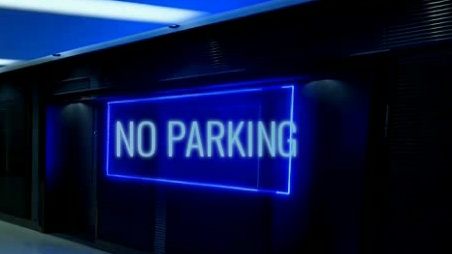
\includegraphics[width=0.146\linewidth]{figs/cells/qual_g029_en_screen_s3_B1.jpg} & 
\includegraphics[width=0.146\linewidth]{figs/cells/qual_g078_zh_screen_s4_orig.jpg} & 
\includegraphics[width=0.146\linewidth]{figs/cells/qual_g078_zh_screen_s4_steervte.jpg} & 
\includegraphics[width=0.146\linewidth]{figs/cells/qual_g078_zh_screen_s4_B1.jpg} \\
&\parbox[t]{0.146\linewidth}{\centering\scriptsize \textcolor{badred}{\ding{55}}\,\texttt{PARKING}} & \parbox[t]{0.146\linewidth}{\centering\scriptsize \textcolor{okgreen}{\ding{51}}\,\texttt{NO PARKING}} & \parbox[t]{0.146\linewidth}{\centering\scriptsize \textcolor{okgreen}{\ding{51}}\,\texttt{NO PARKING}} & \parbox[t]{0.146\linewidth}{\centering\scriptsize \textcolor{badred}{\ding{55}}\,\texttt{\cjkimg{cjk_9107d7aedf}}} & \parbox[t]{0.146\linewidth}{\centering\scriptsize \textcolor{okgreen}{\ding{51}}\,\texttt{\zh{停车场}}} & \parbox[t]{0.146\linewidth}{\centering\scriptsize \textcolor{okgreen}{\ding{51}}\,\texttt{\zh{停车场}}} \\[3pt]
\end{tabular}
\caption{\textbf{Qualitative comparison on randomly sampled clips} (one English and one Chinese clip per material, drawn with a fixed seed among garbled originals outside the development set; not curated). Each cell is the same crop of frame 24; below it, the reader's transcription (\textcolor{okgreen}{\ding{51}}~correct, \textcolor{badred}{\ding{55}}~wrong). SteerVTE produces more natural glyphs but frequently keeps or invents wrong characters; Banksy writes the target but its glyphs often look pasted (see \cref{sec:limits}).}
\label{fig:qual}
\end{figure*}

\begin{figure*}[t]
\centering
\setlength{\tabcolsep}{1.2pt}\renewcommand{\arraystretch}{0.6}
\begin{tabular}{@{}cccccc@{}}
\footnotesize\textbf{Original} & \footnotesize\textbf{SteerVTE} & \footnotesize\textbf{Banksy} & \footnotesize\textbf{Original} & \footnotesize\textbf{SteerVTE} & \footnotesize\textbf{Banksy} \\[2pt]

\includegraphics[width=0.16\linewidth]{figs/cells/wins_g007_en_glass_s7_orig.jpg} & 
\includegraphics[width=0.16\linewidth]{figs/cells/wins_g007_en_glass_s7_steervte.jpg} & 
\includegraphics[width=0.16\linewidth]{figs/cells/wins_g007_en_glass_s7_B1.jpg} & 
\includegraphics[width=0.16\linewidth]{figs/cells/wins_g065_zh_metal_s9_orig.jpg} & 
\includegraphics[width=0.16\linewidth]{figs/cells/wins_g065_zh_metal_s9_steervte.jpg} & 
\includegraphics[width=0.16\linewidth]{figs/cells/wins_g065_zh_metal_s9_B1.jpg} \\
\parbox[t]{0.16\linewidth}{\centering\scriptsize \textcolor{badred}{\ding{55}}\,\texttt{FREESEY BREAD}} & \parbox[t]{0.16\linewidth}{\centering\scriptsize \textcolor{badred}{\ding{55}}\,\texttt{FREESEY BREAD}} & \parbox[t]{0.16\linewidth}{\centering\scriptsize \textcolor{okgreen}{\ding{51}}\,\texttt{FRESH BREAD}} & \parbox[t]{0.16\linewidth}{\centering\scriptsize \textcolor{badred}{\ding{55}}\,\texttt{\zh{使判二}}} & \parbox[t]{0.16\linewidth}{\centering\scriptsize \textcolor{badred}{\ding{55}}\,\texttt{\zh{便刺店}}} & \parbox[t]{0.16\linewidth}{\centering\scriptsize \textcolor{okgreen}{\ding{51}}\,\texttt{\zh{便利店}}} \\[3pt]

\includegraphics[width=0.16\linewidth]{figs/cells/wins_g006_en_paper_s7_orig.jpg} & 
\includegraphics[width=0.16\linewidth]{figs/cells/wins_g006_en_paper_s7_steervte.jpg} & 
\includegraphics[width=0.16\linewidth]{figs/cells/wins_g006_en_paper_s7_B1.jpg} & 
\includegraphics[width=0.16\linewidth]{figs/cells/wins_g105_zh_wood_s2_orig.jpg} & 
\includegraphics[width=0.16\linewidth]{figs/cells/wins_g105_zh_wood_s2_steervte.jpg} & 
\includegraphics[width=0.16\linewidth]{figs/cells/wins_g105_zh_wood_s2_B1.jpg} \\
\parbox[t]{0.16\linewidth}{\centering\scriptsize \textcolor{badred}{\ding{55}}\,\texttt{FRESY BREAD}} & \parbox[t]{0.16\linewidth}{\centering\scriptsize \textcolor{badred}{\ding{55}}\,\texttt{FRESY BREAD}} & \parbox[t]{0.16\linewidth}{\centering\scriptsize \textcolor{okgreen}{\ding{51}}\,\texttt{FRESH BREAD}} & \parbox[t]{0.16\linewidth}{\centering\scriptsize \textcolor{badred}{\ding{55}}\,\texttt{\zh{小吧灯滑} COFFEE}} & \parbox[t]{0.16\linewidth}{\centering\scriptsize \textcolor{badred}{\ding{55}}\,\texttt{\zh{小吧地滑}}} & \parbox[t]{0.16\linewidth}{\centering\scriptsize \textcolor{okgreen}{\ding{51}}\,\texttt{\zh{小心地滑}}} \\[3pt]

\includegraphics[width=0.16\linewidth]{figs/cells/wins_g101_zh_signboard_s3_orig.jpg} & 
\includegraphics[width=0.16\linewidth]{figs/cells/wins_g101_zh_signboard_s3_steervte.jpg} & 
\includegraphics[width=0.16\linewidth]{figs/cells/wins_g101_zh_signboard_s3_B1.jpg} & 
\includegraphics[width=0.16\linewidth]{figs/cells/wins_g064_zh_screen_s8_orig.jpg} & 
\includegraphics[width=0.16\linewidth]{figs/cells/wins_g064_zh_screen_s8_steervte.jpg} & 
\includegraphics[width=0.16\linewidth]{figs/cells/wins_g064_zh_screen_s8_B1.jpg} \\
\parbox[t]{0.16\linewidth}{\centering\scriptsize \textcolor{badred}{\ding{55}}\,\texttt{\cjkimg{cjk_c572b7eb7f} CONOG}} & \parbox[t]{0.16\linewidth}{\centering\scriptsize \textcolor{badred}{\ding{55}}\,\texttt{\zh{公园} COKOO}} & \parbox[t]{0.16\linewidth}{\centering\scriptsize \textcolor{okgreen}{\ding{51}}\,\texttt{\zh{公园}}} & \parbox[t]{0.16\linewidth}{\centering\scriptsize \textcolor{badred}{\ding{55}}\,\texttt{\zh{便判品}}} & \parbox[t]{0.16\linewidth}{\centering\scriptsize \textcolor{badred}{\ding{55}}\,\texttt{\zh{便判台}}} & \parbox[t]{0.16\linewidth}{\centering\scriptsize \textcolor{okgreen}{\ding{51}}\,\texttt{\zh{便利店}}} \\[3pt]
\end{tabular}
\caption{\textbf{Clips that only Banksy repairs} (selected by hand). The examples are chosen among the 41 clips outside the development set that both readers judge wrong in the original and in SteerVTE's output and right in Banksy's; the reverse case---right with SteerVTE and wrong with Banksy under both readers---occurs in 8 clips (failure modes in \cref{fig:fail}). Each cell is the same crop of frame 24, with the first reader's transcription below (\textcolor{okgreen}{\ding{51}}~correct, \textcolor{badred}{\ding{55}}~wrong).}
\label{fig:wins}
\end{figure*}

% Background fidelity: absolute grey-level difference to the original frame (clipped at 24), full frame, frame 24; Banksy = al_r1 B1 outputs.
\begin{figure}[t]
\centering
\setlength{\tabcolsep}{1pt}\renewcommand{\arraystretch}{0.5}
\begin{tabular}{@{}ccc@{}}
\footnotesize Original & \footnotesize $|\,$\steer $-$ original$\,|$ & \footnotesize $|\,$\method $-$ original$\,|$ \\[2pt]

\includegraphics[width=0.325\linewidth]{figs/cells/diff_g106_zh_paper_s6_orig.jpg} &

\includegraphics[width=0.325\linewidth]{figs/cells/diff_g106_zh_paper_s6_steervte_diff.png} &

\includegraphics[width=0.325\linewidth]{figs/cells/diff_g106_zh_paper_s6_B1_diff.png} \\
 & \scriptsize outside: 2.58 & \scriptsize outside: 1.74 \\[2pt]
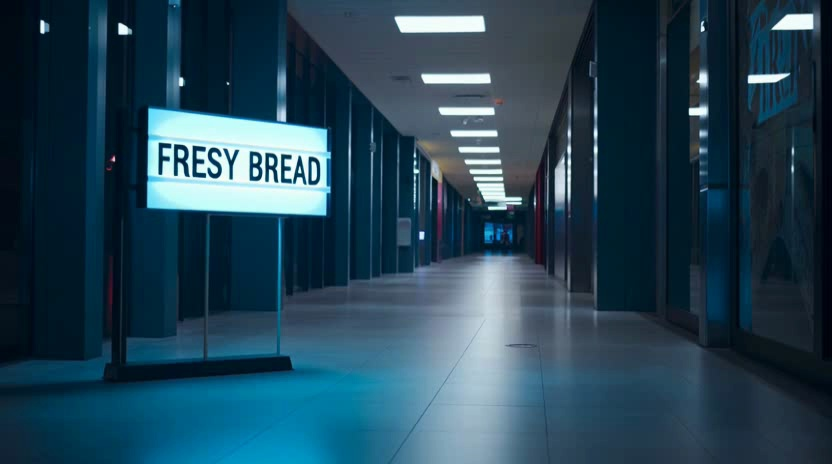
\includegraphics[width=0.325\linewidth]{figs/cells/diff_g008_en_signboard_s4_orig.jpg} &

\includegraphics[width=0.325\linewidth]{figs/cells/diff_g008_en_signboard_s4_steervte_diff.png} &

\includegraphics[width=0.325\linewidth]{figs/cells/diff_g008_en_signboard_s4_B1_diff.png} \\
 & \scriptsize outside: 1.70 & \scriptsize outside: 0.95 \\[2pt]
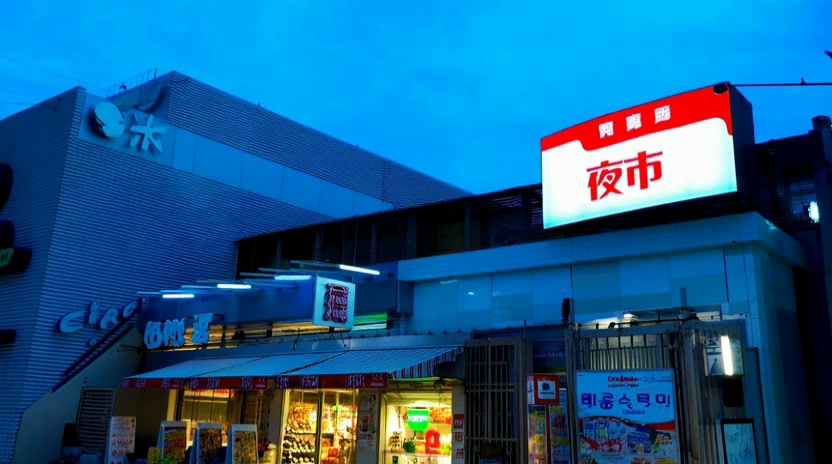
\includegraphics[width=0.325\linewidth]{figs/cells/diff_g085_zh_signboard_s0_orig.jpg} &
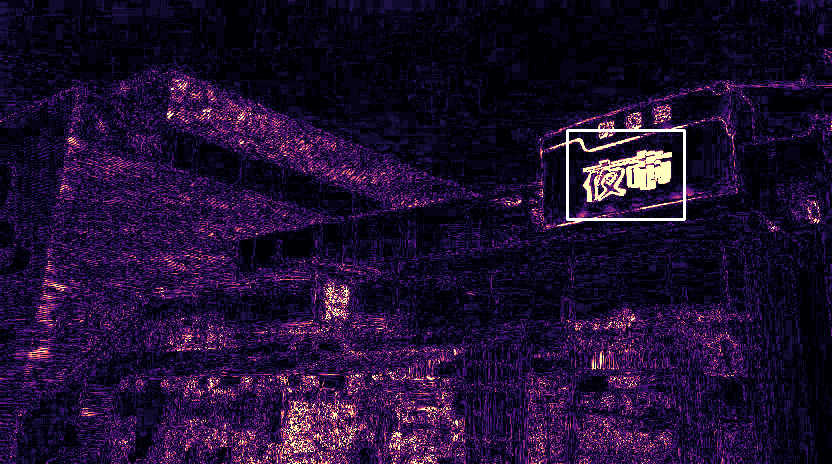
\includegraphics[width=0.325\linewidth]{figs/cells/diff_g085_zh_signboard_s0_steervte_diff.png} &

\includegraphics[width=0.325\linewidth]{figs/cells/diff_g085_zh_signboard_s0_B1_diff.png} \\
 & \scriptsize outside: 2.53 & \scriptsize outside: 0.88 (untouched) \\
\end{tabular}
\caption{\textbf{Edit locality.} Absolute grey-level difference to the original frame (clipped at 24; white box: text region). \steer re-renders the whole frame, so residual edges appear everywhere; \method changes only the text region. The numbers give the mean absolute difference outside the dilated text region. \method's residual there (1--2 grey levels, block artefacts of the output codec) is the video re-encoding floor, visible alone in the bottom row, where the preservation gate leaves an already-correct clip untouched while \steer still alters it.}
\label{fig:diff}
\end{figure}


\subsubsection{Edit locality}
\label{sec:exp_local}
\Cref{fig:diff} visualises where each method changes the video. Because \steer passes the whole clip through its generator, its difference to the original covers the entire frame, including edges of buildings and furniture far from the text; for \method, the difference is confined to the text region, and the residual elsewhere (1--2 grey levels) is the re-encoding of the output video. Inside the neighbourhood of the text, we additionally measure the collateral change---the change outside both the old and the new glyphs---which is \rOursCollat{} grey levels for \method on the \rOursCollatN{} clips it edits; it cannot be computed for \steer, whose glyph coverage is unknown.

\subsubsection{The evidence gates}
\label{sec:exp_gates}
\paragraph{Preservation gate.} The gate skips \rSkipped{} clips, and the reader confirms all \rSkippedOK{} as correct (no false skip; the pre-registered limit was 2\%). Its effect on breakage is measured in the selective-editing pass (\cref{tab:selective}), where it is the only difference between B0 and B1: it restores \sRestored{} of the \sBrokenBzero{} originally correct clips that B0 breaks and loses none (\sBrokenBzero{} vs.\ \sBrokenBone{} broken clips, readability \sReadBzero\% vs.\ \sReadBone\%). Its recall is low by design: it fires on \rSkipped{} of the \rOrigCorrect{} clips the reader judges correct, because the pipeline's OCR rarely reads stylised originals---neon italics, extruded letters, condensed faces---with the required consistency. All \rOursBroken{} originally correct clips that \method breaks are such cases (\cref{sec:failures}).








% Component ablations (earlier front end; experiments T and D, sheets 15-16) and front-end variants (sheet 30), 526 clips.
% Appearance is normalised within each evaluation job, so it is comparable only inside one block.
\begin{table*}[t]
\centering
\begin{minipage}[t]{0.43\linewidth}
\centering
\caption{\textbf{Rendering components} (earlier front end, 526 clips). Top: carrier-anchored temporal components; bottom: style-matched rendering. Appearance is normalised within each block. The box policy used by \method's fallback is T4 + D2.}
\label{tab:components}
\small\setlength{\tabcolsep}{2.4pt}
\resizebox{\linewidth}{!}{%
\begin{tabular}{@{}lcccc@{}}
\toprule
 & Read.\ $\uparrow$ & Flicker $\downarrow$ & Jitter $\downarrow$ & Appear.\ $\downarrow$ \\
\midrule
Original & 53.8 & 1.98 & 9.18 & -- \\
\steer & 83.8 & 1.66 & 8.30 & -- \\
Naive paste (per-frame OCR box) & 87.1 & 3.12 & 11.66 & -- \\
\quad + carrier tracking (T1) & 87.3 & 2.80 & 10.28 & -- \\
\quad + carrier-space erasure (T2) & 88.6 & 2.19 & 9.27 & -- \\
\quad + anchored masks, ink smoothing (T3) & 87.1 & 3.06 & 11.47 & -- \\
\quad + all three (T4) & 89.0 & 1.67 & 7.12 & -- \\
\midrule
\steer & 83.8 & -- & -- & 1.39 \\
Naive paste & 86.9 & -- & -- & 1.89 \\
\quad + font matching (D1) & 89.5 & -- & -- & 1.83 \\
\quad + per-frame ink, shading field (D2) & 89.4 & -- & -- & 1.82 \\
\quad + edge blur and grain (D3) & 87.6 & -- & -- & 2.01 \\
\bottomrule
\end{tabular}}
\end{minipage}\hfill
\begin{minipage}[t]{0.55\linewidth}
\centering
\caption{\textbf{Front-end variants and the localization gate} (526 clips, one evaluation job). W/L: clips correct only with the variant / only with the box policy (McNemar $p$). Residual: share of old ink still visible, relative to the original, on 24 held-out clips.}
\label{tab:frontend}
\small\setlength{\tabcolsep}{2.4pt}
\resizebox{\linewidth}{!}{%
\begin{tabular}{@{}lccccc@{}}
\toprule
 & Read.\ $\uparrow$ & vs.\ box (W/L, $p$) & Jitter $\downarrow$ & Appear.\ $\downarrow$ & Resid.\ $\downarrow$ \\
\midrule
Original & 53.8 & -- & 9.18 & -- & 1.00 \\
\steer & 84.0 & 33/68, $<$.001 & 8.30 & 1.50 & -- \\
Naive paste & 86.7 & 16/37, .005 & 12.53 & 2.38 & -- \\
Box policy (T4+D2) & 90.7 & -- & 7.80 & 2.27 & 0.42 \\
Instance layout, state-machine tracking & 85.2 & 32/61, .003 & 7.68 & 2.50 & 0.21 \\
Instance layout, carrier tracking & 86.9 & 34/54, .042 & 7.68 & 2.44 & -- \\
\quad + localization gate (\method front end) & 91.1 & 27/25, .89 & 7.66 & 2.33 & 0.23 \\
\bottomrule
\end{tabular}}
\end{minipage}
\end{table*}


\paragraph{Carrier anchoring and style-matched rendering.} \Cref{tab:components} ablates the rendering components on an earlier front end. Pasting the target into the per-frame OCR box makes the text readable but nearly doubles flicker relative to the original clip (3.12 vs.\ 1.98), because OCR boxes jitter from frame to frame. Anchoring everything on the tracked carrier removes most of it: carrier-space erasure contributes most ($-0.93$), tracking $-0.32$ and anchored masks with ink smoothing $-0.05$, and the three together reduce flicker by 1.45, more than the sum of their parts, to the level of \steer (1.67 vs.\ 1.66) while lowering jitter well below it (7.12 vs.\ 8.30). Readability does not suffer (89.0 vs.\ 87.1, $p=0.064$). Matching the font to the old strokes adds 2.6 points of readability (D1; $p=0.044$) once candidates are rendered in the layout of the original---an earlier version compared single-line candidates with two-line originals and systematically picked the thinnest faces. Per-frame ink and a shading field (D2) bring the appearance closest among the rendered variants; imitating edge blur and grain (D3) makes text both less readable and less similar, and was dropped. T4 + D2 constitutes the \emph{box policy}, the fallback of \method.

\paragraph{The localization gate.} Laying the text out on the old glyph instance should look more faithful than filling a box, and on held-out clips it does: it leaves half as much of the old ink visible (residual 0.21 vs.\ 0.42 of the original). On all 526 clips, however, the first instance-aligned front end was 5.5 points \emph{less} readable than the box policy (85.2 vs.\ 90.7; \cref{tab:frontend}). Size and colour were not the cause---forcing the box policy's colour pipeline or a minimum letter height left the gap unchanged (supplement)---but its confidence-based tracking state machine was: replacing it by carrier tracking recovers most of the gap on the clips where an instance is found (90.8 vs.\ 91.3), and the remaining clips are those where the instance estimate itself is unreliable. The localization gate routes exactly these clips to the box policy, which yields a front end that is as readable as the box policy (91.1 vs.\ 90.7; 27 vs.\ 25 discordant clips) while keeping the instance path's lower residual (0.23) and lowest jitter (7.66). Two re-readings of the same outputs differ by about one point (90.3 vs.\ 91.3 in a second job), so we claim parity with the box policy, not superiority. A subset of 100 clips had suggested a gain of one point for an earlier gated variant (95 vs.\ 94) that did not replicate on the full set (88.4 vs.\ 91.3)---a reminder that subset gates are optimistic.

\subsection{Source appearance transport}
\label{sec:exp_sat}
% SAT v1 paired results on the 53 clips where the appearance gate enabled it (full 526-clip pass, sheet 33). Paste only = Banksy front end without SAT.
\begin{table}[t]
\centering
\caption{\textbf{SAT on the clips where the appearance gate enables it} (53 of 526; paired, same front-end pass). $\Delta$: SAT $-$ paste only, with 95\% bootstrap CI.}
\label{tab:sat}
\small\setlength{\tabcolsep}{3pt}
\begin{tabular}{@{}lccc@{}}
\toprule
 & Paste only & + SAT & $\Delta$ [95\% CI] \\
\midrule
Readability (\%) & 98.1 & 100 & +1 clip \\
Appearance $\downarrow$ & 2.97 & 1.95 & $-1.02$ [$-1.70$, $-0.48$] \\
Flicker $\downarrow$ & 2.25 & 2.40 & $+0.15$, $p<0.001$ \\
Jitter $\downarrow$ & 8.62 & 9.42 & $+0.81$, $p=0.001$ \\
BG PSNR (dB) & 43.01 & 43.02 & n.s. \\
\bottomrule
\end{tabular}
\end{table}

% SAT: Original / paste only / + SAT (frame 24, tight crops) and the blind human study (53 SAT-enabled clips, 4 raters).
\begin{figure}[t]
\centering
\setlength{\tabcolsep}{1pt}\renewcommand{\arraystretch}{0.5}
\begin{tabular}{@{}m{1.15cm}ccc@{}}
 & \footnotesize Original & \footnotesize Paste only & \footnotesize + SAT \\[2pt]
\scriptsize \str{PHARMACY} & 
\includegraphics[width=0.265\linewidth]{figs/cells/sat_g026_en_signboard_s5_orig.jpg} & 
\includegraphics[width=0.265\linewidth]{figs/cells/sat_g026_en_signboard_s5_paste.jpg} & 
\includegraphics[width=0.265\linewidth]{figs/cells/sat_g026_en_signboard_s5_sat.jpg} \\
\scriptsize \str{CINEMA} & 
\includegraphics[width=0.265\linewidth]{figs/cells/sat_g017_en_signboard_s1_orig.jpg} & 
\includegraphics[width=0.265\linewidth]{figs/cells/sat_g017_en_signboard_s1_paste.jpg} & 
\includegraphics[width=0.265\linewidth]{figs/cells/sat_g017_en_signboard_s1_sat.jpg} \\
\scriptsize \zh{水果店} & 
\includegraphics[width=0.265\linewidth]{figs/cells/sat_g116_zh_screen_s8_orig.jpg} & 
\includegraphics[width=0.265\linewidth]{figs/cells/sat_g116_zh_screen_s8_paste.jpg} & 
\includegraphics[width=0.265\linewidth]{figs/cells/sat_g116_zh_screen_s8_sat.jpg} \\
\scriptsize \zh{营业中}\newline\textcolor{badred}{\tiny failure} & 
\includegraphics[width=0.265\linewidth]{figs/cells/sat_g110_zh_neon_s4_orig.jpg} & 
\includegraphics[width=0.265\linewidth]{figs/cells/sat_g110_zh_neon_s4_paste.jpg} & 
\includegraphics[width=0.265\linewidth]{figs/cells/sat_g110_zh_neon_s4_sat.jpg} \\
\end{tabular}\\[3pt]
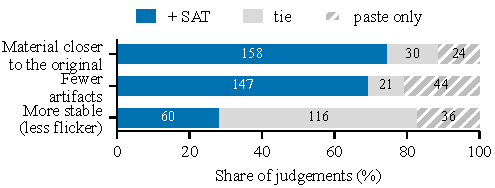
\includegraphics[width=\linewidth]{figs/plots/sat_human.pdf}
\caption{\textbf{Source appearance transport.} Top: SAT carries glow and material of the old glyphs to the new ones (rows 1--3: clips that raters judged better with SAT on both material and artifacts; row 4: a neon clip that all raters judged to have more artifacts with SAT). Bottom: blind pairwise study on all 53 SAT-enabled clips (4 raters, 212 judgements per question; \cref{sec:exp_sat}).}
\label{fig:sat}
\end{figure}


\paragraph{Where the gate enables SAT.} In the pass analysed here, the appearance gate enables SAT on 53 of the 526 clips (in the run of \cref{tab:main}, on \rSatOn): 23 of 93 neon clips, 11 of 65 screens, 9 of 86 signboards, 8 of 56 metal and 2 of 54 wooden signs, and none on glass or paper. Most rejections are clips without an accepted instance (203), followed by non-emissive text (133), no cross-validated gain (104) and gain in only one direction (33). Every enabled clip has a cross-validated error ratio below 0.75 in both directions, and the 15 rejected clips closest to the threshold lie between 0.756 and 0.795.

\paragraph{Effect.} On the enabled clips (\cref{tab:sat}), SAT reduces the appearance distance by a third ($-1.02$; better on 42 of 53 clips) for every material---screens 3.02$\to$1.33, neon 3.03$\to$2.02, wood 4.12$\to$2.21---without hurting readability or the background. It costs temporal stability: flicker rises by 0.15 and jitter by 0.81, because the transported appearance follows a per-frame distance field. On the full benchmark the readability is unchanged (90.5 vs.\ 90.3\%).

\paragraph{Human judgement.} Because the appearance distance is only a proxy, we ran a blind study on all 53 enabled clips (\cref{fig:sat}): raters saw the original between the paste-only and the SAT version in random order and answered three separate questions. Of five raters, one gave the same side on all three questions for 98\% of the clips (including the flicker question, which asks which version is worse) and was excluded by a rule (identical answers on at least 80\% of the clips) that we fixed only after seeing the data; we therefore also report the material question with all five raters. With four raters (212 judgements per question), SAT was judged closer to the original material in 158 cases against 24 (30 ties; win rate 0.87, 95\% CI [0.77, 0.94] by bootstrap over raters and clips; 48 vs.\ 3 clips by majority), and as having fewer artifacts in 147 against 44 (0.77 [0.66, 0.87]); with five raters the material win rate is 0.84 [0.74, 0.92]. Agreement is moderate (Gwet's AC1~\cite{gwet2008ac1} 0.51 for material, 0.61 for artifacts), and the left/right position had no effect after balancing (53\% left, $p=0.27$). The measured flicker increase was not perceived: 55\% of the flicker answers are ties, the remaining answers follow the material answer (a halo effect), and they correlate negatively with the measured flicker change ($\rho=-0.34$). The appearance distance agrees with the material votes only weakly ($\rho=0.28$, $p=0.049$) and not with the artifact votes, so it cannot replace human judgement.

\paragraph{Failures and their cause.} Raters judged six clips to have clearly more artifacts with SAT, four of them neon (\cref{fig:sat}, last row): a bright rectangular plate behind the new letters. A first hypothesis---that the new glyphs reach distances never observed on the old ones---was rejected (the share of unobserved distances is at most 2.3\%), and tapering the operator to identity at the edge of its support had no effect. The plates coincide instead with the canvas on which the new glyphs' distance field is computed: the canvas leaves only 0.04--0.21 letter heights of margin, so the halo, which should extend to 0.6, is cut at the canvas border. With an untruncated distance field the straight edges disappear in our diagnosis, and computing the distance field on a padded canvas reduces flicker by 0.08 and jitter by 0.37 (both better on 47 of 53 clips, $p<0.001$) with no significant change in appearance---about half of SAT's flicker cost and 40\% of its jitter cost. Because these 53 clips were used to diagnose the failure, the padded version is not part of the evaluated \method and requires validation on unseen clips.

\subsection{Selective, structure-preserving editing}
\label{sec:exp_sel}
% generated by make_tab_selective.py from align/sel2/ev1 (one evaluation job for every row)
\begin{table*}[t]
\centering
\caption{\textbf{Selective, structure-preserving editing} (pre-registered; 526 clips; one front-end pass, in which the 99 two-row clips were re-run after a compositing fix, and one evaluation run for every row: all rows read together, every metric computed over all rows at once). B0 is \method without the preservation gate; each component is added to B0 separately and then all three together (B4). Collateral: change outside the old and new glyphs in the text neighbourhood. The verdict applies the pre-registered criteria; development clips are excluded in the right block. The B1 of this pass and the \method of \cref{tab:main} are the same configuration in two independent front-end passes and evaluation runs.}
\label{tab:selective}
\resizebox{\linewidth}{!}{%
\begin{tabular}{@{}lccccccccc|ccc@{}}
\toprule
 & \multicolumn{9}{c|}{All 526 clips} & \multicolumn{3}{c}{486 clips (no development clips)} \\
 & Read.\ $\uparrow$ & Fixed & Broken & Net & Appear.\ $\downarrow$ & BG PSNR & Collateral $\downarrow$ & Flicker & Verdict & Read.\ $\uparrow$ & Net & Collateral $\Delta$ vs.\ B0 \\
\midrule
B0: \method w/o preservation gate & 91.3 & 214 & 16 & 198 & 2.52 & 42.97 & 1.55 & 1.76 & -- & 91.2 & 178 & -- \\
B1: + preservation gate (= \method) & \textbf{91.6} & 214 & \textbf{14} & \textbf{200} & 2.39 & 42.97 & 1.52 & 1.79 & adopted & \textbf{91.4} & \textbf{179} & $-0.031$ [$-0.06$, $-0.01$] \\
B2: + glyph-only erasure & 83.7 & 181 & 23 & 158 & 2.43 & 43.06 & 1.46 & 1.79 & rejected & 84.4 & 145 & $-0.036$ [$-0.09$, $+0.03$] \\
B3: + carrier-fit check & 88.8 & 200 & 15 & 185 & 2.39 & 42.95 & 1.54 & 1.77 & rejected & 88.9 & 167 & $-0.004$ [$-0.01$, $-0.00$] \\
B4: all three & 82.9 & 173 & 19 & 154 & \textbf{2.21} & 43.05 & \textbf{1.43} & 1.82 & rejected & 83.3 & 140 & $-0.062$ [$-0.12$, $+0.01$] \\
\bottomrule
\end{tabular}}
\end{table*}


Inspecting the outputs of the first full evaluation, we found that the most frequent problem of \method was not that its glyphs lacked material but that it changed things it should not have: already-correct text, sign frames, and the structure around the letters. We therefore tested three components that make editing more selective, each added to B0 (\method without the preservation gate) on its own, with acceptance criteria fixed before the run (supplement): the preservation gate of \cref{sec:pres} (B1), \emph{glyph-only erasure} (B2), and a \emph{carrier-fit check} (B3).

\paragraph{Glyph-only erasure (B2).} Instead of inpainting the whole letter band, B2 erases only the old glyphs and their own glow, estimated with a mixture model of carrier, ink and halo colours, and protects sign frames, long bars and the boxes of other text. It is active on the 325 clips with an accepted instance---in 117 of them it falls back to band erasure minus the protected structures, because the surroundings themselves look like strokes (\eg neon stripes)---and its erased area is a median 0.64 of the band area. \emph{Pre-registered criterion}: collateral change decreases ($p<0.05$) and readability drops by at most one point.

\paragraph{Carrier-fit check (B3).} B3 estimates the extent of the carrier from colour, lightness and texture boundaries and declares a clip \emph{layout-infeasible} if the target, at the character density of the source, would have to shrink below 0.7 of the source height to fit; such clips are left unedited and counted as failures. \emph{Criterion}: the infeasible flags are confirmed by manual inspection.

\paragraph{Results.} \Cref{tab:selective} reports all variants from one front-end pass (with the 99 two-row clips re-run after a compositing fix that affects all variants alike). The preservation gate meets its criteria (no false skip; two fewer broken clips; readability not lower) and is adopted, which makes B1 the \method of \cref{tab:main}. Glyph-only erasure reduces collateral change on all clips ($-0.090$, 95\% CI $[-0.17,-0.02]$, $p=0.017$) but not significantly once the development clips are removed ($p=0.23$), and it costs 7.3 points of readability: the instance ink mask is not a complete glyph mask, so parts of the old strokes survive next to the new ones, and OCR boxes of the garbled text itself were sometimes protected as ``other text''. A second version that completes the old glyphs by colour still left remnants in three of nine diagnosed clips, which suggests that this component needs a learned stroke segmentation. Of the 24 clips flagged infeasible by the carrier-fit check, manual inspection confirmed 5, was undecided on 3 and rejected 16 (OCR missed letters of the source, or two-row signs were treated as one row), so B3 is rejected as well; a stricter version that only flags clips whose source stably shows a whole-word part of the target behaved correctly on the diagnosed clips but has not been run at scale. All three together (B4) inherit B2's readability loss. A blind study comparing B1 with \steer (60 clips) and B2 with B0 (28 clips) on naturalness and on damage to non-target content is in progress \pending{(results pending)}.

\subsection{Verified selection between \method and \steer}
\label{sec:exp_hybrid}
% generated by assemble_hybrid.py (one evaluation run; verifier InternVL, scorer Qwen)
\begin{table*}[t]
\centering
\caption{\textbf{Verified selection between \method and \steer} (526 clips; one evaluation run for every row, so \method and \steer are re-evaluated here). Banksy-V keeps the clip when the preservation gate fires, otherwise takes a \steer output (seed 1, then seed 2) whose text an independent verifier (InternVL2.5-8B, the protocol of \cref{sec:metrics}) reads as the target, composited back into the original frame around the text box, and falls back to \method otherwise. Scored by the first reader; the verifier never scores. W/L vs.\ \method: clips correct only with the system / only with \method (McNemar $p$). Pixtral: readability on the 295 English clips under the third reader.}
\label{tab:hybrid}
\setlength{\tabcolsep}{4pt}
\resizebox{\linewidth}{!}{%
\begin{tabular}{@{}lcccccccccc@{}}
\toprule
 & Read.\ $\uparrow$ & Fixed & Broken $\downarrow$ & Net $\uparrow$ & W/L vs.\ \method ($p$) & Appear.\ $\downarrow$ & BG PSNR $\uparrow$ & Flicker $\downarrow$ & Jitter $\downarrow$ & Pixtral $\uparrow$ \\
\midrule
\method (B1) & 91.6 & 212 & 12 & 200 & -- & 3.33 & 42.52 & 1.79 & 7.86 & 77.6 \\
\steer & 84.0 & 165 & 5 & 160 & 30/70 ($7.9\times10^{-5}$) & 2.39 & 36.49 & 1.66 & 8.30 & 80.3 \\
Banksy-V: verified selection, local composite & 96.4 & 225 & 0 & 225 & 31/6 ($4.1\times10^{-5}$) & 2.61 & 41.74 & 1.86 & 8.68 & 87.5 \\
\quad whole-frame instead of local composite & 96.0 & 224 & 1 & 223 & 31/8 ($2.9\times10^{-4}$) & 2.69 & 37.41 & 1.72 & 8.28 & 87.8 \\
\quad seed 1 only & 95.4 & 220 & 0 & 220 & 25/5 ($3.2\times10^{-4}$) & 2.68 & 41.82 & 1.85 & 8.61 & 86.8 \\
Oracle selection (selector = reader; upper bound) & 98.1 & 234 & 0 & 234 & 35/1 ($1.1\times10^{-9}$) & 2.62 & 41.74 & 1.88 & 8.84 & 88.5 \\
\bottomrule
\end{tabular}}
\end{table*}


The two systems fail on different clips (\cref{sec:limits}), so a system that could tell which output is right would inherit the readability of both. We registered one before running it (supplement), with no tunable threshold. \emph{Banksy-V} keeps the clip when the preservation gate fires; otherwise it runs \steer (seed 1, then a second seed) and accepts an output whose text an independent verifier---InternVL2.5-8B with the reading protocol of \cref{sec:metrics}---transcribes as the target in at least 4 of 5 frames; otherwise it falls back to \method. An accepted \steer output is not used as a whole frame: only its text region is composited back into the original, with weight 1 inside the text box and up to 0.3 box heights outside it (shadow and glow), a linear fade over 0.12 box heights, and a per-channel affine colour match to the original on an annulus around the composite. The verifier never scores: readability is reported by the first reader and, on the English clips, by Pixtral, which have no part in the selection. \Cref{tab:hybrid} evaluates every row in one run (the second of two; the first, which contained only the pre-registered variants, gave the same verdicts).

\paragraph{Result.} Banksy-V reads correctly in \hVRead\% of the clips, \hVOnlySys{} vs.\ \hVOnlyBone{} discordant clips against \method (McNemar $p=\hVP$), with \hVBroken{} originally correct clips broken and \hVNet{} net repairs (\method: \hBoneNet; \steer: \hSteerNet); the third reader agrees (\hVPix\% vs.\ \hBonePix\% for \method and \hSteerPix\% for \steer). Its appearance distance (\hVMad) lies between \steer's (\hSteerMad) and \method's (\hBoneMad), because \steer's text is used wherever it reads correctly---in \hVChosensteerlocal{} clips with the first seed and \hVChosensteerTwolocal{} with the second---and the background stays local (\hVBG\,dB against \hVWholeBG\,dB when the whole \steer frame is accepted). The verifier accepted \hFalseAccepts{} outputs that the first reader judges wrong, \hFalseAcceptsBone{} of which \method had right; an oracle that selects with the scoring reader itself reaches \hOracleRead\%, so the verifier closes most of the gap between the two systems. Banksy-V meets five of the six pre-registered criteria; it misses the temporal one by a small margin (flicker \hVFlicker{} vs.\ a limit of 1.85, jitter \hVJitter{} vs.\ 8.40), which the whole-frame variant does not (\hVWholeFlicker{}, \hVWholeJitter): the per-frame colour match of the composite adds frame-to-frame variation. A variant with one colour match per clip, defined after this result, brings flicker within the limit (\hVCFlicker) but not jitter (\hVCJitter); the remaining difference to the whole-frame variant is the re-encoding of the composited output, which the whole-frame row does not undergo: re-encoding \steer's own outputs with our writer raises their flicker by 0.15 and jitter by 0.44, and the per-clip-matched composite is then indistinguishable from them (supplement).

\paragraph{What this does and does not show.} Banksy-V is a system combination: its material comes from \steer, its correctness from verification, and its locality and fallback from \method. It runs \steer (108\,s per clip on its hardware) up to twice per clip plus a 7B-parameter verifier, and it inherits \steer's licence and compute. It does not make \method's own glyphs look more like the original; the material gap of \cref{sec:limits} is unchanged for the \hVChosenBOne{} clips that still come from \method. What it shows is that, on this task, an independent reader is a reliable enough judge of correctness that a generative editor can be used where it is right and avoided where it is wrong.

\subsection{External benchmarks}
\label{sec:exp_external}
Both external evaluations below were run with the earlier box-policy front end (\cref{tab:components}); re-running them with the final pipeline is pending, and we report them as they are.

\paragraph{Editing correct text (VTE-Bench).} On the 100 real clips of \steer's own benchmark~\cite{zeng2026steervte}, where correct text must be changed into a different string, \steer reaches 92\% readability and our earlier pipeline 82\% (8 vs.\ 18 discordant clips, $p=0.076$; a second reader, EasyOCR, gives 49\% vs.\ 44\%). Editing differs from repair: the source text is valid and must be removed entirely, which is the regime that generative editors are trained for and in which our gates provide no advantage. We include the result to delimit our claims.

\paragraph{Commercial video models (VidScribe).} VidScribe~\cite{vidscribe2026} releases the outputs of seven commercial video models for video-to-video text editing. On the 44 of its 93 clips that have a localisable text region, our earlier pipeline reaches 29.5\% (naive paste) and 27.3\% (box policy) readability, ahead of the strongest commercial model (minimax-h3, 18.2\%) and wan-3.0 (15.9\%), although not significantly (box policy vs.\ minimax-h3: 6 vs.\ 2 discordant clips, $p=0.29$); against the other five models (0--13.6\%) the box policy is significantly better ($p\le0.031$). Commercial models regenerate the whole clip and lower the PSNR outside the text region to 19.8--27.9\,dB, against 37.6--37.9\,dB for our outputs. Absolute readability is low for every method because most VidScribe targets are long phrases.

\subsubsection{Analysis and limitations}
\label{sec:analysis}

\begin{figure*}[t]
\centering
\setlength{\tabcolsep}{1.2pt}\renewcommand{\arraystretch}{0.6}
\begin{tabular}{@{}m{2.6cm}ccc@{}}
&\footnotesize\textbf{Original} & \footnotesize\textbf{Banksy} & \footnotesize\textbf{SteerVTE (ref.)} \\[2pt]
\scriptsize Correct original edited anyway; style lost & 
\includegraphics[width=0.27\linewidth]{figs/cells/fail_g043_en_glass_s1_orig.jpg} & 
\includegraphics[width=0.27\linewidth]{figs/cells/fail_g043_en_glass_s1_B1.jpg} & 
\includegraphics[width=0.27\linewidth]{figs/cells/fail_g043_en_glass_s1_steervte.jpg} \\
&\parbox[t]{0.27\linewidth}{\centering\scriptsize \textcolor{okgreen}{\ding{51}}\,\texttt{FLOWER MARKET}} & \parbox[t]{0.27\linewidth}{\centering\scriptsize \textcolor{okgreen}{\ding{51}}\,\texttt{FLOWER MARKET}} & \parbox[t]{0.27\linewidth}{\centering\scriptsize \textcolor{okgreen}{\ding{51}}\,\texttt{FLOWER MARKET}} \\[3pt]
\scriptsize Erase patch, low contrast & 
\includegraphics[width=0.27\linewidth]{figs/cells/fail_g026_en_signboard_s7_orig.jpg} & 
\includegraphics[width=0.27\linewidth]{figs/cells/fail_g026_en_signboard_s7_B1.jpg} & 
\includegraphics[width=0.27\linewidth]{figs/cells/fail_g026_en_signboard_s7_steervte.jpg} \\
&\parbox[t]{0.27\linewidth}{\centering\scriptsize \textcolor{badred}{\ding{55}}\,\texttt{PHARMAICA}} & \parbox[t]{0.27\linewidth}{\centering\scriptsize \textcolor{okgreen}{\ding{51}}\,\texttt{PHARMACY}} & \parbox[t]{0.27\linewidth}{\centering\scriptsize \textcolor{okgreen}{\ding{51}}\,\texttt{PHARMACY}} \\[3pt]
\scriptsize Outlined 3D letters flattened & 
\includegraphics[width=0.27\linewidth]{figs/cells/fail_g014_en_wood_s3_orig.jpg} & 
\includegraphics[width=0.27\linewidth]{figs/cells/fail_g014_en_wood_s3_B1.jpg} & 
\includegraphics[width=0.27\linewidth]{figs/cells/fail_g014_en_wood_s3_steervte.jpg} \\
&\parbox[t]{0.27\linewidth}{\centering\scriptsize \textcolor{okgreen}{\ding{51}}\,\texttt{EXIT}} & \parbox[t]{0.27\linewidth}{\centering\scriptsize \textcolor{okgreen}{\ding{51}}\,\texttt{EXIT}} & \parbox[t]{0.27\linewidth}{\centering\scriptsize \textcolor{okgreen}{\ding{51}}\,\texttt{EXIT}} \\[3pt]
\scriptsize New text overflows the sign & 
\includegraphics[width=0.27\linewidth]{figs/cells/fail_g010_en_neon_s5_orig.jpg} & 
\includegraphics[width=0.27\linewidth]{figs/cells/fail_g010_en_neon_s5_B1.jpg} & 
\includegraphics[width=0.27\linewidth]{figs/cells/fail_g010_en_neon_s5_steervte.jpg} \\
&\parbox[t]{0.27\linewidth}{\centering\scriptsize \textcolor{okgreen}{\ding{51}}\,\texttt{BOOK STORE}} & \parbox[t]{0.27\linewidth}{\centering\scriptsize \textcolor{badred}{\ding{55}}\,\texttt{K STORE}} & \parbox[t]{0.27\linewidth}{\centering\scriptsize \textcolor{okgreen}{\ding{51}}\,\texttt{BOOK STORE}} \\[3pt]
\scriptsize Second row missed; old text remains & 
\includegraphics[width=0.27\linewidth]{figs/cells/fail_g058_en_signboard_s4_orig.jpg} & 
\includegraphics[width=0.27\linewidth]{figs/cells/fail_g058_en_signboard_s4_B1.jpg} & 
\includegraphics[width=0.27\linewidth]{figs/cells/fail_g058_en_signboard_s4_steervte.jpg} \\
&\parbox[t]{0.27\linewidth}{\centering\scriptsize \textcolor{okgreen}{\ding{51}}\,\texttt{TEA HOUSE}} & \parbox[t]{0.27\linewidth}{\centering\scriptsize \textcolor{badred}{\ding{55}}\,\texttt{TEA TEA HOUSE}} & \parbox[t]{0.27\linewidth}{\centering\scriptsize \textcolor{okgreen}{\ding{51}}\,\texttt{TEA HOUSE}} \\[3pt]
\scriptsize Neon glyph blurred & 
\includegraphics[width=0.27\linewidth]{figs/cells/fail_g076_zh_neon_s7_orig.jpg} & 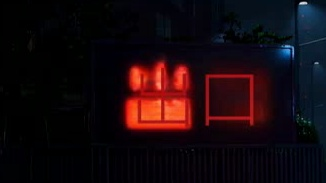
\includegraphics[width=0.27\linewidth]{figs/cells/fail_g076_zh_neon_s7_B1.jpg} & 
\includegraphics[width=0.27\linewidth]{figs/cells/fail_g076_zh_neon_s7_steervte.jpg} \\
&\parbox[t]{0.27\linewidth}{\centering\scriptsize \textcolor{okgreen}{\ding{51}}\,\texttt{\zh{出口}}} & \parbox[t]{0.27\linewidth}{\centering\scriptsize \textcolor{badred}{\ding{55}}\,\texttt{\zh{备份}}} & \parbox[t]{0.27\linewidth}{\centering\scriptsize \textcolor{okgreen}{\ding{51}}\,\texttt{\zh{出口}}} \\[3pt]
\end{tabular}
\caption{\textbf{Failure modes of Banksy} (hand-picked to cover each type; SteerVTE shown for reference). The first three keep the target readable but degrade appearance; the last three come from clips whose original was already correct and that Banksy broke.}
\label{fig:fail}
\end{figure*}


\subsubsection{Where \method fails}
\label{sec:failures}
\paragraph{Breaking correct text.} \method breaks \rOursBroken{} of the \rOrigCorrect{} originally correct clips (\steer: \rSteerBroken). In all of them, the evaluation reader transcribes the original correctly while the pipeline's OCR reads it correctly in at most 2\% of the frames (neon italics, extruded or condensed letters), so the preservation gate cannot fire. Inspecting the outputs (\cref{fig:fail}, last three rows) gives four failure types: new text larger than its sign, so that letters fall off the carrier (4 clips); old text left visible next to the new text, because a second row was not detected or the erasure was incomplete (5); wrong colour or contrast on lightboxes and extruded letters (2); and stacked two-row text on an LED screen that is still misread (1). In one of these clips the reader's verdict on the original is itself doubtful: the original shows a garbled four-character string, which the reader transcribes as \zh{电影院} in every frame.

\paragraph{Readable but not faithful.} The more common failure does not affect readability (\cref{fig:fail}, first three rows): erasure leaves a visible patch, or the new glyphs are flat where the old ones were outlined, extruded or glowing. These cases are frequent in the random sample of \cref{fig:qual} and explain the appearance distance in \cref{tab:main}.

\subsubsection{The appearance gap to generative editing}
\label{sec:limits}
Among the \rBothRepairN{} garbled clips that both methods repair, \steer's text is closer to the original appearance in \rSteerCloserPct\% (median appearance distance \rBothRepairMedSteer{} vs.\ \rBothRepairMedOurs), so the gap is not an artefact of \steer leaving garbled text untouched. We see four causes, in decreasing order of visibility.
\begin{itemize}
\item \textbf{Rendering instead of generation.} \method can reproduce colour, shading and, with SAT, glow; it cannot reproduce extrusion, bevels, tube geometry or texture inside the strokes, which a generator synthesises naturally.
\item \textbf{A small font library.} The library holds 33 Latin and 8 Chinese families, and the generator's typefaces are invented. In practice, \rLatinFam{} Latin families are selected, but for Chinese only \rZhFam, and Noto Sans SC alone renders \rNotoPct\% of the edited Chinese clips; the result reads correctly but looks uniform. Choosing the font by the shapes of the identifiable source letters (\cref{sec:exp_neg}) changed the font in only \rFshapeN{} clips.
\item \textbf{Axis-aligned layout.} The letter band inherits the orientation of the OCR quad, which is axis-aligned for most detectors, so on tilted carriers the new text can look skewed relative to the sign (\cref{fig:teaser}a); the perspective estimate of an earlier front end was too fragile to keep (supplement), and laying the text along the source baseline (\cref{sec:exp_neg}) could not be shown to help with our appearance metric, which does not see orientation.
\item \textbf{Erasure traces.} LaMa fills the hole once per clip; on textured or shaded carriers the fill is visible as a patch.
\end{itemize}
Two observations suggest that the gap is closable without giving up correctness. First, the garbled source already contains most of the target's characters: in garbled English clips, a median of \rCharsEn\% of the target letters occur in the reader's transcription of the original (Chinese: \rCharsZh\%). Reusing these glyphs---with their own font, colour, lighting and perspective---and synthesising only the missing ones would extend the ``change only what is wrong'' principle from words to characters; our first implementation (\cref{sec:exp_neg}) shows that the bottleneck is reliable letter segmentation and matching, which currently admits too few clips. Second, the two methods fail on different clips: the share of clips that at least one of them repairs is \rAtLeastOne\%. A combination that accepts a generative edit only when independent OCR verifies it, and otherwise falls back to deterministic repair, is a natural next step; its verifier must be strict, since accepting a wrong edit costs correctness, whereas rejecting a right one costs only appearance.

\subsubsection{Other limitations}
The benchmark is generated by one family of models and its prompts ask for short sign texts; a second generator (CogVideoX-5B, 360 clips from the same prompts) is part of our plan but has not been evaluated yet, and long texts such as menus or user interfaces are out of scope. Readability is measured by a VLM reader; it favours large, high-contrast text, which may flatter rendered glyphs, and it can transcribe a garbled original as the intended word (\cref{sec:failures}). A pre-registered second reader from another model family confirms the advantage over \steer, with a smaller margin that is significant for Chinese but not for English alone, and a third reader limited to English finds the methods level once its invented additions are discounted (\cref{sec:main}); readability claims therefore depend on the reader, and we report all of them. The appearance distance is glyph-agnostic and has a test--retest noise of \rRetestSD{} per clip (\cref{sec:exp_neg}): it supports large differences such as the gap to \steer and the effect of SAT, but not small ones. The human study on SAT used four raters after quality control; a registered blind comparison of \method with \steer on material naturalness, artifacts and temporal stability was not conducted for lack of raters, so the appearance comparison with \steer rests on the appearance distance and on visual examples. Finally, the preservation gate is safe but has low recall, because it relies on a conventional OCR that rarely reads stylised originals. Outside repair, on editing correct text (VTE-Bench), the frozen system is clearly behind \steer (\xVteOurs\% vs.\ \xVteSteer\%, \cref{sec:exp_external}), partly because its front end fails to locate \xVteFails{} of the 100 source texts.


\section{Negative results in full}
\label{sec:supp_neg}
\subsection{Does a learned refiner help?}
\label{sec:exp_refiner}
% Learned refiner on the 526 clips, all rows read in one evaluation job (workbook sheet 31, complete version).
% W/L vs the same front end without the refiner. Appearance normalised within this job.
\begin{table}[t]
\centering
\caption{\textbf{Does a learned refiner help?} The 1.3B bridge-flow refiner applied on top of \method's front end (paste only) and of the box policy, with and without the carrier-anchored attention bias ($\lambda=2$). 526 clips, one evaluation job; W/L against the same front end without the refiner. Boundary jump: change at the refiner's 17-frame chunk seams relative to other frame pairs (1 = no seam).}
\label{tab:refiner}
\resizebox{\linewidth}{!}{%
\begin{tabular}{@{}lcccccc@{}}
\toprule
 & Read.\ $\uparrow$ & W/L & Flicker $\downarrow$ & Jitter $\downarrow$ & B.\ jump $\downarrow$ & Appear.\ $\downarrow$ \\
\midrule
\steer & 84.2 & -- & 1.66 & 8.34 & 0.93 & 1.58 \\
\midrule
\method front end (paste only) & 91.3 & -- & 1.77 & 7.69 & 0.84 & 2.49 \\
\quad + refiner & 87.8 & 3/21 & 1.96 & 8.22 & 2.26 & 2.45 \\
\quad + refiner + attention bias & 88.6 & 3/17 & 2.00 & 8.41 & 2.06 & 2.33 \\
\midrule
Box policy (paste only) & 91.4 & -- & 1.77 & 7.83 & 0.84 & 2.35 \\
\quad + refiner & 87.6 & 2/22 & 1.99 & 8.46 & 2.31 & 2.31 \\
\quad + refiner + attention bias & 88.4 & 3/19 & 2.03 & 8.68 & 2.10 & 2.24 \\
\bottomrule
\end{tabular}}
\end{table}


Rendered glyphs look pasted, so the obvious remedy is to let a generative model harmonise them with the scene while keeping their shapes. We invested heavily in this route before settling on the training-free pipeline, and report it in full because its outcome shapes our design.

\paragraph{Refiner.} The refiner is a video diffusion transformer initialised from Wan2.1-T2V-1.3B~\cite{wan2025wan} that takes the pasted clip as extra input channels (zero-initialised) and is trained as a flow-matching bridge~\cite{lipman2023flowmatching,liu2023rectifiedflow} from the paste to the target; inference starts from the paste, in the spirit of SDEdit~\cite{meng2022sdedit}, and takes 30 Euler steps on 17-frame chunks of $384\times384$ crops. A glyph loss compares Sobel edges of the decoded prediction with the target inside a band around the glyph (weighted by the signed distance to the glyph boundary). Training pairs come from three sources: a Blender data factory with six carrier surfaces and passing occluders, which renders every sample twice (lit composite and flat paste); 562 real pairs obtained by erasing correct text from generated clips and re-pasting it; and up to 1.15 million image pairs built the same way from AnyWord-3M (63\% LAION, 31\% Wukong, 6\% street scenes). All refiners were trained on H100-class GPUs (GH200/H200) for 20k steps.

\paragraph{More data is not the lever.} On a 296-clip garbled subset, refiners trained with 0, 10k, 100k and 1M image pairs reach 78.4, 75.3, 76.4 and 76.4\% readability, all below the paste they start from (80.7\%), and their appearance does not improve with data (supplement). A diagnostic on 1{,}500 held-out pairs explains why: on the very task they were trained for---turning the paste back into the original---all of them move \emph{away} from the original, they do not even memorise pairs seen twelve times, and they fail to learn a systematic difference (originals have thicker strokes than our pastes in 60\% of the pairs). The supervision was inconsistent: the paste uses our font, the target uses the generator's, and the glyph loss, which dominates the objective, effectively teaches the model to erase our strokes. Making the supervision glyph-consistent---pasting the original's own ink mask instead of our font---is the first recipe that moves toward the original on held-out pairs and it cuts the image-domain readability loss from 26 to 4 points, with appearance better than the paste. On videos, however, it still does not exceed the paste (best variant: 79.7 vs.\ 80.7\%).

\paragraph{System-level effect.} \Cref{tab:refiner} applies the best refiner to the full benchmark. On top of \method's front end it costs 3.5 points of readability (21 clips broken against 3 repaired; $p<0.001$), increases flicker and jitter, and introduces seams at its chunk boundaries (boundary jump 2.26 vs.\ 0.84), while the appearance distance does not change significantly ($-0.035$, 95\% CI $[-0.21, 0.19]$). A training-free attention bias that ties tokens to their carrier trajectory, in the spirit of flow-guided attention~\cite{cong2024flatten,geyer2024tokenflow}, was selected on 50 clips with an earlier refiner (boundary jump $-16\%$ there) and reduces the seams by 9\% on the full set (2.06 vs.\ 2.26; better on 364 of 526 clips), but it slightly increases flicker within chunks and leaves the readability loss in place. We therefore keep the refiner out of \method. The negative result is specific to our scale---1.3B parameters and at most a few hundred real video pairs, against a 14B backbone and a million training triplets for \steer---but it is consistent: at this scale, a learned harmoniser trades the guarantee that motivates rendering for an appearance gain we could not measure.

\subsection{Two appearance modules that did not pass}
\label{sec:exp_neg}
% generated by paper_numbers.py: frozen variants from r1full (same front-end pass and evaluation job as Table 1)
\begin{table}[t]
\centering
\caption{\textbf{Two appearance modules that did not pass their pre-registered criteria} (same front-end pass and evaluation job as \cref{tab:main}). $\Delta$App.: paired appearance difference to B1 with 95\% bootstrap CI, on the clips outside both development sets (477 clips); the criterion required the upper bound to be below 0. R1 changed 7 clips, 5 of them development clips.}
\label{tab:reuse}
\setlength{\tabcolsep}{3pt}
\resizebox{\linewidth}{!}{%
\begin{tabular}{@{}lcccc@{}}
\toprule
 & Read.\ $\uparrow$ & Net $\uparrow$ & App.\ $\downarrow$ & $\Delta$App.\ vs.\ B1 \\
\midrule
\method (B1, final) & 91.4 & 198 & 2.57 & -- \\
+ baseline layout + glyph-shape font (B1f) & 91.3 & 197 & 2.61 & $+0.052$ [$+0.002$, $+0.106$] \\
+ source-glyph reuse (R1) & 91.4 & 198 & 2.56 & $+0.021$ [$-0.023$, $+0.067$] \\
+ both (R1f) & 91.3 & 197 & 2.57 & $+0.034$ [$-0.016$, $+0.092$] \\
\bottomrule
\end{tabular}}
\end{table}


Two of the causes of the appearance gap (\cref{sec:limits}) look addressable without generation: the new text ignores the orientation and the typeface of the old one, and the garbled source already contains most of the target's letters. We built one module for each and fixed their acceptance criteria before running them on the benchmark (supplement). Both were run in the same front-end pass and evaluation job as \cref{tab:main}, so every comparison in \cref{tab:reuse} is paired.

\paragraph{Baseline-aligned layout and glyph-matched fonts (B1f).} The first component lays the new text along the baseline of the old glyphs instead of the axis-aligned OCR quad, when two ink-based angle estimates agree within $2^\circ$ and the rotation lies between $2^\circ$ and $20^\circ$. The second chooses the typeface by the shapes of the source letters whose identity can be established---the multi-frame consensus reading aligned to the target---and replaces the matched font only if the best per-letter overlap is at least 0.6 (English, single row). The criteria were: readability at most one point lower, a paired appearance difference whose 95\% CI lies below zero, and perceived naturalness not worse in a later human study. The text was rotated in \rTiltN{} clips and the font replaced in \rFshapeN; elsewhere the output equals B1. Readability is unchanged (0 vs.\ 1 discordant clips), but the appearance difference is $\rBOnefMadDiffND$ [$\rBOnefMadLoND$, $\rBOnefMadHiND$] on the clips outside both development sets, so the second criterion is not met and B1f is not adopted. Under the current evaluation protocol we observe no overall benefit; its perceptual effect has not been verified. We do not read this as evidence that font or orientation alignment is ineffective, for two reasons. First, the appearance distance is glyph-agnostic by construction (colour, contrast, halo, edge softness and shading inside the strokes, \cref{sec:metrics}): it does not see typeface similarity or text orientation, which are exactly what B1f changes. Choosing it as the criterion for these components was an error in our pre-registration, which we report rather than amend after the fact. Second, the distance is not deterministic: its ink segmentation runs $k$-means with random initialisation, and on the \rRetestN{} clips where R1 leaves the output byte-identical to B1, the two scores agree exactly in only \rRetestSame{} clips, differ with a standard deviation of \rRetestSD{} per clip, and differ by $\rRetestMean$ [$\rRetestLo$, $\rRetestHi$] on average. B1f's difference is of the same order as this test--retest noise. Deciding whether B1f looks better requires its own pre-registered human study.

\paragraph{Source-glyph reuse (R1).} R1 keeps the source letters that are already correct in place---with their own pixels, font, material and perspective---erases only the wrong span between them, and renders only the missing letters, in a font chosen to match the kept ones. It acts only when the evidence is strong: the number of segmented source letters equals the reading, at least half of the target letters are kept, the kept letters are read stably across frames, no letter must be inserted or deleted between kept letters, the new letters' shapes match the kept ones (overlap at least 0.65), and the new text stays on its carrier; otherwise the clip keeps the B1 output. R1 was applied to \rReuseApplied{} of the 526 clips (\rReuseGarbledEn{} of the \rGarbledEn{} garbled English clips), \rReuseAppliedDev{} of them development clips. On the two others the appearance distance improved by \rReuseNDMad{} with unchanged readability, which is far too few clips to evaluate the criteria. The limiting factor is coverage: in \rReuseWhyLetters{} English clips the segmented letters did not match the reading, in \rReuseWhySource{} the pipeline's consensus reading of the source already equalled the target, and in \rReuseWhyFont{} no font matched the kept letters well enough. With our current letter segmentation, matching and gating, reuse applies to too few clips to form a general module. This bounds the implementation, not the idea; the 20\% coverage observed on a 30-clip sample before the full run did not hold on the benchmark.

Both modules are frozen and are not part of \method, which in \cref{tab:main} is B1.

\paragraph{Reconstruction without source glyphs.} \method's evidence gating assumes that some glyph survives. Classifying the benchmark with the frozen localiser (supplement), \lthreeGlyphs{} clips have readable matches, \lthreeLtwo{} have detectable but unreadable pseudo-text, and none lacks a detectable text-like region; \method reads \lthreeLtwoBoneRead\% of the pseudo-text clips through its detection-box fallback (\steer: \lthreeLtwoSteerRead\%). We additionally investigated glyph-free, carrier-conditioned text reconstruction, which lays the target out from the tracked carrier alone, with no glyph mask, OCR box or letter height. The first registered branch, evaluated on the \lthreeGlyphs{} clips with their glyphs erased, read \lthreeACarRead\% of the locatable clips where the frozen code's static-hint fallback reads \lthreeABfbRead\%, but missed the registered geometry and stability criteria (\lthreeAPassed{} of \lthreeACriteria); two further registered rounds also failed (\cref{sec:supp_g_rounds}). A fourth version, designed on a separate development set, was frozen and evaluated once on a sealed set of clips from two other generators (CogVideoX-5B and Wan2.2-TI2V-5B; \gTSynN{} glyph-erased clips with geometry truth and \gTNatN{} natural pseudo-text clips; \cref{sec:supp_g4_t4}). It improved readability by \gTReadGainU{} percentage points over the static-hint fallback (95\% CI \gTReadGainLo{} to \gTReadGainHi), read more of the natural pseudo-text clips than the deployed \method on both generators, and kept the background within \gTBgMaxGap\,dB of an identity re-encoding. However, it did not satisfy all acceptance criteria registered before the test set was opened: text-scale consistency failed on CogVideoX (median height ratio \gTCogHeight) and temporal non-inferiority on one stability measure per generator. We therefore retain the evidence-gated B1 system as our primary method and report glyph-free reconstruction as an exploratory extension.

\begin{figure}[t]
\centering
\setlength{\tabcolsep}{1.2pt}\renewcommand{\arraystretch}{0.6}
\begin{tabular}{@{}m{2.4cm}ccc@{}}
&\footnotesize\textbf{Original} & \footnotesize\textbf{Banksy} & \footnotesize\textbf{Generator} \\[2pt]
\scriptsize closer than Banksy (metal) & 
\includegraphics[width=0.3\linewidth]{figs/cells/mg_g117_zh_metal_s1_orig.jpg} & 
\includegraphics[width=0.3\linewidth]{figs/cells/mg_g117_zh_metal_s1_B1.jpg} & 
\includegraphics[width=0.3\linewidth]{figs/cells/mg_g117_zh_metal_s1_matgen.jpg} \\
&\parbox[t]{0.3\linewidth}{\centering\scriptsize \textcolor{badred}{\ding{55}}\,\texttt{\zh{邮局}}} & \parbox[t]{0.3\linewidth}{\centering\scriptsize \textcolor{okgreen}{\ding{51}}\,\texttt{\zh{邮局}}} & \parbox[t]{0.3\linewidth}{\centering\scriptsize \textcolor{okgreen}{\ding{51}}\,\texttt{\zh{邮局}}} \\[3pt]
\scriptsize farther (LED sign) & 
\includegraphics[width=0.3\linewidth]{figs/cells/mg_g085_zh_signboard_s8_orig.jpg} & 
\includegraphics[width=0.3\linewidth]{figs/cells/mg_g085_zh_signboard_s8_B1.jpg} & 
\includegraphics[width=0.3\linewidth]{figs/cells/mg_g085_zh_signboard_s8_matgen.jpg} \\
&\parbox[t]{0.3\linewidth}{\centering\scriptsize \textcolor{badred}{\ding{55}}\,\texttt{\zh{夜市} Qingdao Night Marke}} & \parbox[t]{0.3\linewidth}{\centering\scriptsize \textcolor{okgreen}{\ding{51}}\,\texttt{\zh{夜市}}} & \parbox[t]{0.3\linewidth}{\centering\scriptsize \textcolor{okgreen}{\ding{51}}\,\texttt{\zh{夜市}}} \\[3pt]
\scriptsize unreadable (poster) & 
\includegraphics[width=0.3\linewidth]{figs/cells/mg_g025_en_paper_s2_orig.jpg} & 
\includegraphics[width=0.3\linewidth]{figs/cells/mg_g025_en_paper_s2_B1.jpg} & 
\includegraphics[width=0.3\linewidth]{figs/cells/mg_g025_en_paper_s2_matgen.jpg} \\
&\parbox[t]{0.3\linewidth}{\centering\scriptsize \textcolor{badred}{\ding{55}}\,\texttt{PHARMATCE}} & \parbox[t]{0.3\linewidth}{\centering\scriptsize \textcolor{okgreen}{\ding{51}}\,\texttt{PHARMACY}} & \parbox[t]{0.3\linewidth}{\centering\scriptsize \textcolor{badred}{\ding{55}}\,\texttt{PHARMACY}} \\[3pt]
\end{tabular}
\caption{\textbf{The material generator on real clips} (gate R2; three hand-picked examples; Original / Banksy / generator, with the reader's transcription). Trained only on rendered pairs, the generator keeps the glyphs (their alpha is an input) but writes them with low contrast and desaturated colour on most carriers, which the appearance distance and the reader both penalise; it is closer to the original than Banksy only on metal.}
\label{fig:matgen}
\end{figure}

\paragraph{A glyph-locked material generator.} The appearance gap invites a learned module that keeps \method's glyphs and generates only their material. We built one and registered four gates for it (supplement). Counterfactual pairs rendered in Blender---one scene, material and camera path with two strings, so that only the text differs (2{,}000 training pairs over 8 carrier materials, 5 text styles and 41 fonts; 80 validation pairs with the benchmark's target strings, which training excludes)---train a conditional U-Net in the carrier's UV space that receives the erased background, the target glyph alpha and the other string's rendered material and predicts the text layer; the alpha fixes identity, layout and topology. On held-out pairs the model closes 0.48 of the gap between a flat paste and the rendered truth with a glyph IoU of 0.95, below the registered 0.50; the one registered capacity test (1.8$\times$ the parameters, same data, seed and schedule) closes 0.498. Applied zero-shot to the 129 benchmark clips outside the development sets that both \method and \steer repair (\cref{fig:matgen}), it fails every registered criterion: appearance distance 3.06 against 1.99 for \method (paired $+1.08$, 95\% CI $[+0.73, +1.45]$; closer than \method on 24\% of the clips) and 20 readings lost (84.5\% vs.\ 100\%). Under our registered protocol, increasing model capacity by 1.8$\times$ did not close the synthetic-domain criterion, and zero-shot transfer to generated videos substantially degraded both appearance and readability. A registered photometric ablation with the frozen weights (supplement) attributes part of the transfer loss to the renders' photometry---bright, low-contrast text---and leaves the rest unexplained by it; the calibrated output is still farther from the original than a flat paste of the source's median colour. We stop at the gates. The result bounds this generator, data and recipe, not learned material transfer in general, and the glyph-agnostic appearance distance is insensitive to structure, so improvements it cannot see may exist.


\section{Evidence classes and reconstruction without source glyphs}
\label{sec:supp_l3}
Registered on 2026-10-23, after the material generator was closed and before any run; amendments are dated below. \textbf{Question.} With the target string known, can the text be written correctly, in place and stably when no reliable glyph exists, from the carrier alone? \textbf{Evidence classes.} The frozen localiser of \cref{sec:method} was run once on the intact benchmark, restricted to matches inside the hint box: a clip is \emph{glyphs} when the target is matched on at least 20\% of its frames, \emph{pseudo-text} when the detector finds text boxes inside the hint on at least 20\% of the frames but nothing matches, and \emph{glyph-free} otherwise. Of the 526 clips, \lthreeGlyphs{} are glyphs, \lthreeLtwo{} pseudo-text and \lthreeLthree{} glyph-free. In our selected benchmark, every clip contains an OCR-detectable text-like region, although \lthreeLtwo{} clips lack a reliable transcription; this is a property of this generator, this selection rule and this detector, and a missing detection would not have meant that the text had visually vanished. In the run of \cref{tab:main}, \method reads \lthreeGlyphsBoneRead\% of the glyphs clips and \lthreeLtwoBoneRead\% of the pseudo-text clips (through its detection-box fallback), \steer \lthreeGlyphsSteerRead\% and \lthreeLtwoSteerRead\%. The registered natural glyph-free experiment and its routing regression are therefore empty; both were cancelled before any output existed.

\textbf{The branch.} Inputs are the clip, the frame-0 hint box (the same box the fallback uses; never the per-frame boxes) and the target. The carrier is tracked by SIFT homographies around the hint (the estimator of the \emph{track} flag; a clip is \emph{locatable} when it succeeds on at least 80\% of the frames), its extent is scanned outward from the hint on the middle frame with the rules of the carrier-fit module (colour, texture and image-edge boundaries) using the hint's core as the carrier colour, and the text box is laid out deterministically inside that extent (height at most the hint's and 0.6 of the usable height, the string's own aspect ratio, at most 0.86 of the usable width, centred on the hint). Ink is a contrast colour against the carrier, stroke 0.12 of the text height, no glow; the hint region is erased once on the middle frame and carried by the carrier homographies; the glyph canvas of \cref{sec:method} is rendered through the same homographies. The branch never sees glyph masks, OCR boxes, letter heights or source colours.

\textbf{Experiment A, synthetic glyph-free clips.} For the \lthreeGlyphs{} glyphs clips the tracked source quads are the geometry truth; the input is the clip with that quad erased (LaMa once on the middle frame, carried by the quad homographies: \method's own erase), the frame-0 hint and the target. Comparator: the frozen code with its static-hint fallback enabled (\texttt{GL\_FALLBACK=mask}); the deployed configuration ships an unlocated clip unchanged and is reported too (it located \lthreeADepN{} of the 455 clips and read \lthreeADepRead\% of those). Criteria, all required: readability at most one point below the fallback; per-frame IoU with the truth higher (paired CI above zero) and centre drift lower (CI below zero); BG PSNR $\geq 41$\,dB; flicker within $0.05$ and jitter within $0.2$ of the fallback; judged on the locatable clips. \textbf{Result} (\cref{tab:l3}): on the \lthreeALoc{} locatable clips the branch reads \lthreeACarRead\% against \lthreeABfbRead\% (\lthreeAWins{} vs.\ \lthreeALosses{} discordant, $p=\lthreeAP$), keeps the background (\lthreeACarBG\,dB) and lands closer to the old text's centre (\lthreeACarOffset{} vs.\ \lthreeABfbOffset{} text heights, drift \lthreeACarDrift{} vs.\ \lthreeABfbDrift), but its box is not closer to the truth (IoU \lthreeACarIoU{} vs.\ \lthreeABfbIoU, paired \lthreeAIoUMean{} [\lthreeAIoULo, \lthreeAIoUHi]; it renders the text at \lthreeACarHeightRatio{} of the original height) and it is less stable (flicker \lthreeAFlickerMean{} [\lthreeAFlickerLo, \lthreeAFlickerHi], jitter \lthreeAJitterMean{} [\lthreeAJitterLo, \lthreeAJitterHi] above the fallback): \lthreeAPassed{} of \lthreeACriteria{} criteria, \textbf{not passed}. The truth is the old text's footprint, not the optimal layout of the new string, so the IoU criterion is a consistency check only; we report it as registered. The \lthreeANotLoc{} non-locatable clips are reported separately. \textbf{Post hoc} (second run, registered after the result). The true text motion is small (287 of 455 clips move by less than 0.3\,px per frame) and the tracker's velocity error (0.22\,px per frame) equals the motion itself; frames without a SIFT estimate fell back to the static hint, producing jumps. Interpolating across failed frames, smoothing over 9 frames and holding the reference quad when the carrier hardly moves gives readability \lthreeAtwoRead\%, flicker \lthreeAtwoFlicker{} (within the limit) and jitter \lthreeAtwoJitter{} (\lthreeAtwoJitterPMean{} [\lthreeAtwoJitterPLo, \lthreeAtwoJitterPHi] above the fallback, still outside), IoU \lthreeAtwoIoU: the temporal instability was partly attributable to noisy carrier tracking under near-static camera motion. The registered verdict stands.

\textbf{Leakage audit of the synthetic clips.} On the middle frame, the old ink (the colour segmentation of \cref{sec:metrics} on the intact frame) is compared with the other pixels of the old quad after erasure. By the rule fixed before the audit (gradient ratio above 1.5 or a mean luminance difference above 5 levels) \lthreeAuditFlagOrig{} of \lthreeAuditN{} clips are flagged; the gradient ratio has median \lthreeAuditGradMedian{} (no glyph-shaped edges) and the luminance difference median \lthreeAuditDlumMedian{} levels. A revised rule comparing the old ink with a ring around it and with the ink--luminance correlation flags \lthreeAuditFlagRev{} (\lthreeAuditBoth{} in common); the four clips with the strongest correlation show cleanly erased text and a carrier structure (window frames, box edges) inside the old quad; the reader's similarity to the target on the erased inputs is 0 in median. Both counts are kept. Splitting by the original rule, the branch reads \lthreeAuditSuspectCar\% against \lthreeAuditSuspectBfb\% on the flagged clips and \lthreeAuditLowCar\% against \lthreeAuditLowBfb\% on the others: its advantage does not depend on residual cues, but the erased carriers keep low-frequency brightness differences in about half of the clips, which we record as a limitation of the synthetic protocol.

\textbf{Amendment B$'$, natural pseudo-text clips} (registered once the classes were known, before any output of the branch). The branch against \method's deployed outputs on the \lthreeLtwo{} pseudo-text clips, with the criteria of the cancelled natural experiment: readability not significantly worse, no more broken clips, BG PSNR $\geq 41$\,dB, flicker and jitter not worse in CI. Readability \lthreeBCarRead\% vs.\ \lthreeBBoneRead\% (\lthreeBWins{} vs.\ \lthreeBLosses{} discordant, $p=\lthreeBP$), broken \lthreeBCarBroken{} vs.\ \lthreeBBoneBroken, BG \lthreeBCarBG\,dB, flicker and jitter within CI: \textbf{passed}; the branch repairs all \lthreeBFailures{} clips \method fails and loses one. The readability gain is not statistically significant at this size and is bought with appearance: the distance rises from \lthreeBBoneMad{} to \lthreeBCarMad{} (\lthreeBMadMean{} [\lthreeBMadLo, \lthreeBMadHi]), since the branch renders flat text without \method's material modules. A diagnostic run that renders \method's own per-frame layout through the branch's erase and renderer reads \lthreeDiagOcrRead\%, so the gain comes from the layout source (carrier extent vs.\ detection boxes: \lthreeDiagWins{} vs.\ \lthreeDiagLosses, $p=\lthreeDiagP$) and not from the erase; the comparison is nevertheless branch-level.

\textbf{Reproducibility note.} The same frozen code, re-run on the pseudo-text clips in the second environment (OpenCV 4.11, CUDA 12.6, V100; the deployed outputs come from OpenCV 4.12, CUDA 12.8, A40), reads \lthreeBBrerunRead\% instead of \lthreeBBoneRead\% (\lthreeRerunWins{} vs.\ \lthreeRerunLosses{} discordant) with BG PSNR \lthreeBBrerunBG{} instead of \lthreeBBoneBG\,dB. Clip by clip, the decoded frames are identical, the erase masks agree (IoU \xenvMaskIoU), the layout quads agree (\xenvGeomPx\,px) and the OCR quads coincide, but the font matcher chooses a different typeface in \xenvFontDiff{} of \xenvN{} clips and the OCR instance decision differs in a few (letters equal in \xenvLettersSame, gate in \xenvGateSame), so the glyph alphas agree only to IoU \xenvAlphaIoU{} and no output frame is bit-identical (PSNR \xenvPsnrIn\,dB inside the text window, \xenvPsnrOut{} outside). A same-environment repeat is bit-exact. The front end is deterministic within an environment and sensitive to library versions at the font-matching step; B$'$ is therefore reported against the deployed outputs and against the same-environment re-run (\lthreeBrWins{} vs.\ \lthreeBrLosses{} discordant, BG \lthreeBrBGMean{} [\lthreeBrBGLo, \lthreeBrBGHi]).

\textbf{Verdict.} B1 remains the system. The branch is an exploratory capability with a stated boundary: it writes readable text where the deployed system writes nothing, and it does so from the carrier alone, but it has not shown that it can do so without losing material and some temporal stability, and it is not merged. The registered routing regression was not triggered; the exploratory routing study follows.

\textbf{Pseudo-text routing impact study (exploratory; not the registered regression).} All 526 clips in one evaluation run: \method (B1) against a tree that keeps B1 on the \lthreeGlyphs{} glyphs clips and routes the \lthreeLtwo{} pseudo-text clips to the branch (the 455 shared outputs are the same files, with no discordant reading). Readability \cexBoneRead\% $\to$ \cexCexRead\% (\cexWins{} vs.\ \cexLosses{} discordant clips, $p=\cexP$), net repairs \cexBoneNet{} $\to$ \cexCexNet, broken clips \cexBoneBroken{} $\to$ \cexCexBroken; BG PSNR \cexBoneBG{} $\to$ \cexCexBG\,dB (\cexBGMean{} [\cexBGLo, \cexBGHi]); flicker and jitter unchanged (\cexFlickerMean{} [\cexFlickerLo, \cexFlickerHi], \cexJitterMean{} [\cexJitterLo, \cexJitterHi]); appearance distance \cexBoneMad{} $\to$ \cexCexMad{} over all clips (\cexMadMean{} [\cexMadLo, \cexMadHi]) and \cexBoneLtwoMad{} $\to$ \cexCexLtwoMad{} on the routed clips, rising in every material (most on screens, metal and wood). With the post-hoc tracking on the routed clips the temporal metrics improve slightly (flicker \cexCexAFlicker, jitter \cexCexAJitter) and nothing else changes. The routing buys about one point of readability and two fewer broken clips with a measurable loss of appearance on the routed clips and a small loss of background fidelity; by the judgement fixed before this run, B1 remains the system and the branch is not merged.
\IfFileExists{tables/tab_l3.tex}{\begin{table}[t]
\centering\small\setlength{\tabcolsep}{4pt}
\caption{Carrier-grounded reconstruction without source glyphs (supplement). A: the 445 synthetic glyph-free clips whose carrier the branch can track (one evaluation run; the post-hoc row is a second run). B$'$: the 71 pseudo-text clips of the benchmark (one run). Readability by the first reader; BG PSNR in dB; temporal metrics as in Tab.~1.}
\label{tab:l3}
\resizebox{\linewidth}{!}{%
\begin{tabular}{lcccc}
\toprule
Row & Read\,$\uparrow$ & BG\,$\uparrow$ & Flicker\,$\downarrow$ & Jitter\,$\downarrow$\\
\midrule
\multicolumn{5}{l}{\textit{A: synthetic glyph-free clips, locatable carriers (445)}}\\
Erased input & 0.0 & -- & 1.81 & 7.16\\
Frozen \method, static-hint fallback & 81.6 & 41.8 & 2.26 & 8.81\\
Carrier branch (registered) & 92.1 & 41.6 & 2.73 & 12.36\\
Carrier branch, post-hoc tracking (second run) & 92.1 & 41.6 & 2.30 & 10.41\\
\midrule
\multicolumn{5}{l}{\textit{B$'$: natural pseudo-text clips (71)}}\\
Original & 32.4 & -- & 2.05 & 9.38\\
\method (deployed outputs) & 90.1 & 42.4 & 1.75 & 7.86\\
\method re-run, same code & 93.0 & 41.0 & 1.76 & 7.91\\
Carrier branch & 98.6 & 41.2 & 1.67 & 7.87\\
\bottomrule
\end{tabular}}
\end{table}
}{}


% Glyph-free reconstruction after the first registered branch: rounds v2/v3, v4 design, criteria amendment, v4.1 and the sealed
% cross-generator test (numbers: numbers_g4.tex, generated by tools/make_numbers_g4.py). Part of Sec. D of the supplement.
% generated by tools/make_numbers_g4.py -- do not edit by hand
\begin{table*}[t]
\centering\small\setlength{\tabcolsep}{4pt}
\caption{All rounds of the glyph-free branch. Each verdict was taken by criteria fixed before that round's test run and none was revised afterwards. Readability: branch vs.\ comparator on the round's test data (first reader). D4 is development data of v4 and v4.1 and is not a test.}
\label{tab:g_rounds}
\resizebox{\linewidth}{!}{%
\begin{tabular}{lp{4.6cm}p{4.4cm}p{3.3cm}p{4.4cm}}
\toprule
Round & What changed & Test data & Readability & Registered verdict\\
\midrule
v1 & carrier-only layout, SIFT tracking & \lthreeALoc{} synthetic glyph-free clips (benchmark); \lthreeLtwo{} pseudo-text clips & \lthreeACarRead{} vs.\ \lthreeABfbRead{} (fallback); \lthreeBCarRead{} vs.\ \lthreeBBoneRead{} (\method) & not passed: \lthreeAPassed{} of \lthreeACriteria{} criteria met (geometry and stability missed)\\
v2 & motion-model selection; in-carrier layout with a font search & 449 synthetic clips (benchmark); 260 CogVideoX pseudo-text clips & 66.1 vs.\ 81.3; 55.4 vs.\ 78.1 & not passed: readability, IoU, height ratio 1.27, jitter; the font search chose display and calligraphic faces\\
v3 & v2 tracking; frozen default fonts & 57 locatable CogVideoX synthetic clips; the benchmark's 71 pseudo-text clips & 89.5 vs.\ 75.4; 98.6 vs.\ 90.1 & not passed: synthetic 6 of 8 criteria failed; pseudo-text only BG (40.67\,dB $<$ 41\,dB)\\
v4 (v4-LT) & dense-flow tracker with keyframe anchors; layout in carrier $\cap$ allowed region & D4 (development, two generators) & -- & not a test; on D4 two implementation violations of the edit-support constraint were found\\
v4.1 & unified region compositor; inward feather; outside-region invariant & sealed T4: 265 synthetic and 631 pseudo-text clips, two generators & pooled +20.0 pp [+14.8, +25.5] over the fallback & not passed: 3 of 34 gates failed (CogVideoX height ratio and normalised jitter; Wan2.2 normalised flicker)\\
\bottomrule
\end{tabular}}
\end{table*}


\subsection{Rounds v2 and v3}
\label{sec:supp_g_rounds}
After the first registered branch failed (above), two more rounds were registered on 2026-10-24, each before its own test run; \cref{tab:g_rounds} lists every round with its verdict. \textbf{v2} replaced the per-frame tracking by one choice per clip among a static, a homography and a dense-flow trajectory, each smoothed jointly over the clip and selected by its held-out photometric error with a 10\% margin over the static one, and laid the text out inside the carrier with a font search that maximised the text height. On the \gVtwoSynN{} locatable synthetic clips of the benchmark it read \gVtwoSynRead\% against \gVtwoSynFb\% for the static-hint fallback (v1 in the same run: \gVoneSynRead\%). The tracking change alone kept the readability (\gVtwoAoneRead\%) and the layout change alone lost it (\gVtwoAtwoRead\%): the font search chose condensed, display and calligraphic faces that the reader could not read and enlarged the text (median height ratio \gVtwoHeight). On \gVtwoNatN{} pseudo-text clips generated by CogVideoX-5B it read \gVtwoNatRead\% against \gVtwoNatBone\% for \method. \textbf{v3} kept the tracking and returned to the frozen default fonts. Because its design drew on the v2 diagnostics, it was tested on two sets it had never been run on: \gVthreeSynN{} locatable synthetic clips built from CogVideoX-5B clips (of \gVthreeSynAll) and the \lthreeLtwo{} pseudo-text clips of the benchmark. It read \gVthreeSynRead\% against \gVthreeSynFb\% (\gVthreeWins{} vs.\ \gVthreeLosses{} discordant clips, $p=\gVthreeP$) but failed \gVthreeFailed{} of \gVthreeCriteria{} synthetic criteria, with jitter \gVthreeJit{} [\gVthreeJitLo, \gVthreeJitHi] above the fallback; on the pseudo-text clips it read \gVthreeLtwoRead\% against \gVthreeLtwoBone\% ($p=\gVthreeLtwoP$) and failed only the background criterion (\gVthreeLtwoBg\,dB against a limit of 41\,dB), because a layout that follows the carrier can extend beyond the region outside which the background is measured. Both verdicts stand.

Diagnostics run while designing v4---on the v1--v3 outputs, the CogVideoX synthetic set and the development set D4 below, never on the sealed set---explained three recurring failures. (i)~The registered jitter and flicker scale with the edge energy inside the text box: the branch writes high-contrast text where the fallback often writes faint or no text, so their raw difference mostly measures rendering contrast; normalised by edge energy, no branch version was less stable than the fallback. (ii)~The hint box describes frame~0, but every version had used it as the text position on the middle frame, which displaces the text on moving clips by the motion between the two frames. (iii)~IoU with the old text's footprint favours the fallback whenever the hint box is derived from that footprint. These findings changed the metrics and the method of v4, never an earlier verdict.

\subsection{v4: constrained carrier-space reconstruction}
\label{sec:supp_g_v4}
\textbf{Goal and data.} v4 was registered on 2026-10-24 with the requirement that correctness, geometric stability and edit locality improve together, and with the rule that the branch enters \method only if it passes a sealed test. Prompts were generated once: the development set D4 uses 20 target strings and 3 scene templates, the sealed set T4 another 20 strings and 3 templates, each string in four of the seven materials (80 prompts per set); neither set shares a string or a template with the other or with the benchmark's 40 strings and 5 templates. Every prompt was rendered by CogVideoX-5B (50 steps, guidance 6, 720$\times$480, 49 frames at 8\,fps) and Wan2.2-TI2V-5B (40 steps, guidance 5, 832$\times$480, 49 frames at 24\,fps), with fixed seeds: 2 per prompt for D4 and 6 for T4. T4 was raised from 2 to 6 seeds before any of its clips was classified, because 2 seeds would have left fewer than the registered 60 synthetic clips per generator. The frozen localiser classifies every clip; clips with readable matches are erased as in v1 to give synthetic glyph-free clips with geometry truth, pseudo-text clips form a natural subset that is judged separately, and clips without a detectable text region are only counted.

\textbf{Method.} The inputs are the clip, the frame-0 hint box and the target, as in v1. \emph{Tracking:} each step is estimated by dense optical flow inside the carrier region with a per-point forward--backward check (2\,px), at least 30\% consistent points and 30 inliers; sequential RANSAC fits up to two motion layers and keeps the one with the lower photometric error on the carrier core, provided it beats the identity by a factor of 1.15. Keyframes are re-localised against the pre-warped reference to anchor drift, sparse SIFT matches replace the flow where it fails, and the trajectory is fused from anchors, bidirectional chains, interpolation and hold. Each clip chooses a smoothing window of 3, 7 or 13 frames by photometric error (7 unless another is at least 1\% better), and is tracked rather than kept static only with at least three anchors, coverage $\geq 0.5$, an excursion of at least 1\,px and a photometric margin of 0.10. The frame-0 hint is mapped to the reference (middle) frame through the estimated motion. \emph{Layout:} the feasible region is the carrier's extent (scanned as in v1, inset by 0.08 text heights) intersected with the allowed region---the hint box dilated by the larger of 4\,px and half its height, i.e.\ the region outside which background PSNR is measured---back-projected to the reference frame through the trajectory. One to three lines are chosen by matching the text box's aspect ratio to the hint's; a single line is at most the hint's height and 0.75 of the usable height, several lines at most 0.85 of it, and the width at most 0.92; text that would fall below the larger of 12\,px and 0.2 hint heights falls back to \method. Fonts are the frozen defaults of v3; ink and erasure are as in v1.

\textbf{Design.} Every design choice used only the v1--v3 outputs, the CogVideoX synthetic diagnostic set and D4. Dense flow replaced sparse feature chains because generated carriers are smooth (on a quarter of the moving synthetic clips SIFT found no reliable feature); the hint mapping removed the displacement of (ii); the per-clip smoothing reconciled synthetic clips, whose erased region moves with smoothed truth geometry, with natural ones; and the readability floor was lowered from 0.35 to 0.2 hint heights after it had rejected readable text on large hints. T4 was not opened during the design.

\subsection{Acceptance criteria and their amendment}
\label{sec:supp_g_criteria}
The criteria registered with v4 were amended once, after the D4 calibration and before any T4 clip was classified or inspected. The amendment is labelled a \emph{prospective amendment after D4 calibration}, not part of the original registration; it changes no earlier verdict, and D4 counts as development evidence only. It made four changes. (1)~\emph{Correctness:} superiority is tested on the two generators pooled with equal weights (CI lower bound above zero and at least $+5$ points), with non-inferiority per generator (CI lower bound $\geq -5$ points), because the static fallback alone read 93\% on the Wan2.2 part of D4 and left no room for a per-generator superiority test; the pooled readability must also reach v3's. On natural pseudo-text the branch must be non-inferior to the deployed \method per generator (CI lower bound $\geq -5$ points). (2)~\emph{Background:} relative to an identity re-encoding through the same decoder, encoder and region, per generator and subset (no-op $-0.3$\,dB), because even an identity re-encoding stays below 41\,dB on Wan2.2 clips; the paired differences to the fallback and to the deployed \method are reported. (3)~\emph{Tracking:} a controlled experiment with identical fonts, layout, erased background, colour and compositing that differs only in the trajectory (new tracker vs.\ the trajectory selection of v2/v3), judged on natural pseudo-text, because the erased regions of synthetic clips move with smoothed truth geometry and favour smooth trajectories. (4)~\emph{Containment:} mean containment of the text in the carrier of at least 0.90 and non-inferior to the fallback (CI lower bound $\geq -0.03$), with the original 95\% kept as a reported control, plus a separate severe-failure gate (human-confirmed, at most 5\% per generator) and a layout-acceptability gate. Temporal stability is judged by edge-normalised jitter and flicker relative to the fallback (CI upper bound $\leq 0$ per generator, i.e.\ per frame rate), for reason (i); raw values are reported. Geometry requires lower centre offset, drift and motion error than the fallback (CI upper bound below zero) and a median text-height ratio in $[0.8, 1.2]$; IoU and corner error are reported only. All CIs come from a bootstrap that resamples prompts within each generator (10{,}000 resamples, seed 0, percentile intervals), because the seeds of one prompt are correlated; synthetic and natural subsets are never pooled.

\subsection{v4.1: two locality fixes before the sealed test}
\label{sec:supp_g_v41}
On D4 the frozen v4 failed two automatic gates on CogVideoX: the background of the natural subset (\gDCogNatBgVfour{} against \gDCogNatBgNoop\,dB for the identity re-encoding) and the median height ratio (\gDCogHeight). The background failure came from two implementation violations of the registered rule that every edit, including antialiasing and erasure, stays inside the allowed region: the fallback copied the deployed system's whole output, which also changes pixels outside the region (\gCCogLeakFrac\% of the outside pixels and \gCCogLeakShare\% of the total change on the CogVideoX fallback clips), and the clipping feather reached about 3\,px beyond the region. v4.1 corrects exactly these two points. One compositor serves the branch and the fallback: outside the allowed region the output equals the decoded input, the feather runs inward only (opacity given by the exact Euclidean distance to the region boundary over 3\,px), and every frame is compared with the input outside the region before encoding, aborting the job on any difference. Fonts, sizes, layout, tracking, photometric models, smoothing, routing, fallback selection and every threshold are unchanged, and nothing was based on T4. The record states: \emph{``Version v4.1 corrects two implementation violations of the previously specified edit-support constraint, identified during D4 calibration. All changes were completed before inspecting T4 outcomes. The original v4-LT development results and all evaluation thresholds remain unchanged.''} On D4 the outside-region check passed on all \gCCogChecked{} CogVideoX and \gCWanChecked{} Wan2.2 outputs, the layouts were identical to those of v4, the background of the fallback clips relative to the identity re-encoding moved from \gCCogFbBgBefore{} to \gCCogFbBgAfter\,dB (CogVideoX, \gCCogFbN{} clips) and from \gCWanFbBgBefore{} to \gCWanFbBgAfter\,dB (Wan2.2, \gCWanFbN{} clips) with unchanged readability, and no output of the branch itself changed its reading. The natural-subset background then passed on CogVideoX (\gDCogNatBgVfourone\,dB) and the pooled development readability gain was \gDReadGain{} points [\gDReadGainLo, \gDReadGainHi]; the height ratio stayed at \gDCogHeight{} and was not tuned, so v4.1 entered the sealed test with one known automatic failure on D4. The code was frozen with a SHA-256 manifest; the v4 code and its D4 results are kept.

% generated by tools/make_numbers_g4.py -- do not edit by hand
\begin{table*}[t]
\centering\small\setlength{\tabcolsep}{4pt}
\caption{Sealed cross-generator test of the glyph-free branch v4.1: every registered gate, per generator (one run of the frozen code; prompt-clustered 95\% bootstrap CIs; differences are v4.1 minus the frozen code's static-hint fallback on the same erased inputs, or minus the deployed \method on natural pseudo-text). Synthetic: 109 (CogVideoX-5B, 36 prompts) and 156 (Wan2.2-TI2V-5B, 64 prompts) clips. The pooled primary gate (equal-weight mean of the two generators) is +20.0 points [+14.8, +25.5] (passed). A1: the trajectory selection of v2/v3. \ding{55}: failed gate. The two human gates could no longer change the verdict and were replaced by a diagnostic audit (Sec.~\ref{sec:supp_g4_audit}).}
\label{tab:g4}
\resizebox{\linewidth}{!}{%
\begin{tabular}{llrcrc}
\toprule
Gate & Threshold & CogVideoX-5B (8\,fps) & & Wan2.2-TI2V-5B (24\,fps) & \\
\midrule
\multicolumn{6}{l}{\textit{Correctness (synthetic glyph-free; natural pseudo-text is a separate task)}}\\
Readability gain over the static fallback, pp & CI lo $\geq -5$ & +26.6 [+18.1, +36.0] & \ding{51} & +13.5 [+7.5, +19.6] & \ding{51} \\
Natural pseudo-text: gain over deployed \method, pp & CI lo $\geq -5$ & +9.5 [+5.4, +13.8] & \ding{51} & +15.7 [+10.1, +21.5] & \ding{51} \\
\multicolumn{6}{l}{\textit{Temporal stability and locality}}\\
Edge-normalised jitter, difference to fallback & CI hi $\leq 0$ & \ensuremath{-}0.032 [\ensuremath{-}0.072, +0.014] & \textbf{\ding{55}} & \ensuremath{-}0.024 [\ensuremath{-}0.041, \ensuremath{-}0.008] & \ding{51} \\
Edge-normalised flicker, difference to fallback & CI hi $\leq 0$ & \ensuremath{-}0.069 [\ensuremath{-}0.113, \ensuremath{-}0.037] & \ding{51} & \ensuremath{-}0.001 [\ensuremath{-}0.033, +0.055] & \textbf{\ding{55}} \\
BG PSNR synthetic / identity re-encoding, dB & $\geq$ no-op $-0.3$ & 41.38 / 41.55 & \ding{51} & 40.77 / 40.87 & \ding{51} \\
BG PSNR natural / identity re-encoding, dB & $\geq$ no-op $-0.3$ & 41.26 / 41.37 & \ding{51} & 40.43 / 40.51 & \ding{51} \\
Spill outside the allowed region, \% & $\leq 2$ & 0.0 & \ding{51} & 0.0 & \ding{51} \\
Frame overflow, \% (fallback) & $\leq$ fallback & 0.0 (10.1) & \ding{51} & 1.3 (15.4) & \ding{51} \\
\multicolumn{6}{l}{\textit{Tracking and geometry}}\\
Same rendering, new tracker $-$ A1: raw jitter & $\leq +0.2$ & \ensuremath{-}0.52 [\ensuremath{-}0.92, \ensuremath{-}0.20] & \ding{51} & \ensuremath{-}2.04 [\ensuremath{-}2.56, \ensuremath{-}1.56] & \ding{51} \\
Same rendering, new tracker $-$ A1: raw flicker & $\leq +0.05$ & \ensuremath{-}0.080 [\ensuremath{-}0.143, \ensuremath{-}0.031] & \ding{51} & \ensuremath{-}0.340 [\ensuremath{-}0.434, \ensuremath{-}0.252] & \ding{51} \\
Centre offset, difference to fallback & CI hi $< 0$ & \ensuremath{-}0.134 [\ensuremath{-}0.191, \ensuremath{-}0.086] & \ding{51} & \ensuremath{-}0.053 [\ensuremath{-}0.087, \ensuremath{-}0.020] & \ding{51} \\
Drift, difference to fallback & CI hi $< 0$ & \ensuremath{-}0.151 [\ensuremath{-}0.369, \ensuremath{-}0.028] & \ding{51} & \ensuremath{-}0.008 [\ensuremath{-}0.018, \ensuremath{-}0.002] & \ding{51} \\
Motion error, difference to fallback & CI hi $< 0$ & \ensuremath{-}0.073 [\ensuremath{-}0.129, \ensuremath{-}0.033] & \ding{51} & \ensuremath{-}0.014 [\ensuremath{-}0.026, \ensuremath{-}0.006] & \ding{51} \\
Median text-height ratio & $[0.8, 1.2]$ & 0.730 & \textbf{\ding{55}} & 0.965 & \ding{51} \\
\multicolumn{6}{l}{\textit{Containment in the carrier}}\\
Mean containment (fallback) & $\geq 0.90$ & 0.989 (0.971) & \ding{51} & 0.945 (0.917) & \ding{51} \\
Containment, difference to fallback & CI lo $\geq -0.03$ & +0.018 [+0.007, +0.030] & \ding{51} & +0.028 [+0.011, +0.045] & \ding{51} \\
Severe-failure audit; layout acceptability & human & 3 automatic candidates & -- & 12 automatic candidates & -- \\
\bottomrule
\end{tabular}}
\end{table*}


\subsection{The sealed cross-generator test}
\label{sec:supp_g4_t4}
\textbf{Protocol.} T4 was generated after the freeze, and its clips were classified and processed only by the frozen code. Before each generator's run, a content-based isolation audit confirmed that no T4 target string occurs in the development data, that the development folders hold only development prompts, and that no method output existed for T4; the full pipeline then ran once per generator and the verdict was computed once. Of the 480 clips per generator, CogVideoX-5B gave \gTCogLone{} clips with readable matches, \gTCogLtwo{} with pseudo-text and \gTCogLthree{} without a text region, Wan2.2-TI2V-5B \gTWanLone, \gTWanLtwo{} and \gTWanLthree. The synthetic subsets hold \gTCogN{} and \gTWanN{} clips (\gTCogPrompts{} and \gTWanPrompts{} prompts), the natural subsets \gTCogNatAll{} and \gTWanNatAll{} (\gTCogNatN{} and \gTWanNatN{} with a deployed \method output). Every clip is evaluated, including the tracker's localisation failures (\gTCogLocFail\% and \gTWanLocFail\%); no synthetic clip fell back to \method.

\textbf{Results} (\cref{tab:g4}). The branch reads \gTCogRead\% and \gTWanRead\% of the synthetic clips against \gTCogReadFb\% and \gTWanReadFb\% for the static fallback and \gTCogReadVthree\% and \gTWanReadVthree\% for v3; the pooled gain is \gTReadGain{} points [\gTReadGainLo, \gTReadGainHi] (CogVideoX \gTCogReadGain, Wan2.2 \gTWanReadGain). On natural pseudo-text it reads \gTCogNatRead\% and \gTWanNatRead\% against \gTCogNatBone\% and \gTWanNatBone\% for the deployed \method (\gTCogNatGain{} [\gTCogNatGainLo, \gTCogNatGainHi] and \gTWanNatGain{} [\gTWanNatGainLo, \gTWanNatGainHi] points) and breaks \gTCogNatBroken{} and \gTWanNatBroken{} originally readable clips where \method breaks \gTCogNatBoneBroken{} and \gTWanNatBoneBroken. Its background stays within \gTBgMaxGap\,dB of the identity re-encoding in both subsets of both generators; the deployed \method is lower on the natural clips (\gTCogBgNatBone{} and \gTWanBgNatBone\,dB) because its detection-box layout is not restricted to the allowed region used here. With identical rendering, the new tracker lowers the raw jitter relative to the trajectory selection of v2/v3 (\gTCogCtrlJit{} and \gTWanCtrlJit), and it places the text closer to the truth than the fallback in offset, drift and motion error on both generators. Mean containment is \gTCogCont{} and \gTWanCont{} (fallback \gTCogContFb{} and \gTWanContFb); the original 95\% standard is reached on CogVideoX and not on Wan2.2. Three registered gates fail: on CogVideoX the median height ratio is \gTCogHeight{} (D4: \gDCogHeight) and the CI of the normalised jitter difference reaches \gTCogJitNHi; on Wan2.2 the CI of the normalised flicker difference reaches \gTWanFlkNHi. The raw jitter and flicker are higher than the fallback's on both generators (CogVideoX \gTCogJitRaw{} and \gTCogFlkRaw, Wan2.2 \gTWanJitRaw{} and \gTWanFlkRaw), as expected from the higher-contrast rendered text, which is why the normalised measures are the registered gates. The automatic rules flag \gTCogSevere{} and \gTWanSevere{} synthetic clips as severe-failure candidates, all by the crossing rule (containment below 0.80) and none by clipping or missing characters; they are candidates, not confirmed failures.

\textbf{Verdict.} \gTGatesFailed{} of the \gTGatesTotal{} automatic gates fail, so the registered verdict is a failure whatever the two human gates, still pending on both generators, would show. By the decision table fixed before the test, v4.1 is not merged into \method, its results are reported per generator as measured, and it is not modified after the unsealing. Glyph-free reconstruction remains an exploratory extension, and \method (B1) remains the method of this paper.

\subsection{Diagnostic human audit}
\label{sec:supp_g4_audit}
Because the human gates could no longer change the verdict, the registered severe-failure audit was replaced by a smaller diagnostic audit, fixed before any rating: every automatic candidate (\gTCogSevere{} CogVideoX, \gTWanSevere{} Wan2.2) and 30 clips per generator from the unflagged pool, stratified by prompt with a fixed seed, 75 clips in total. Each clip is judged by exactly 3 of 12 independent raters (225 judgements) on one page that shows the input with the allowed region, the edited clip and the target, and shows neither the method nor the candidate status. Question~1 asks whether a severe geometric problem occurs---text on the wrong carrier or crossing carriers, severe clipping or overflow, covering adjacent objects, damage to the carrier's structure; question~2 asks whether the layout is plausible and matches the carrier's geometry. Font aesthetics and material are explicitly not severe. A clip counts as severe (layout acceptable) when at least 2 of its 3 raters say so; raw labels and Fleiss' $\kappa$ are reported. The audit describes what the automatic candidates are and gives a small random-sample picture; it cannot establish a population rate of severe failures, and a candidate the raters do not confirm is not counted as a failure. \pending{Results are added when the ratings are complete.}


\section{Pre-registrations}
\label{sec:supp_prereg_all}
\subsection{Pre-registration of the selective-editing study}
\label{sec:supp_prereg}
The study was registered before the run in an internal document with dated revisions. \textbf{Criteria.} B1: fewer broken clips, false skips $\leq$2\% of the skipped clips, paired readability not lower than B0 by more than 0.5 points. B2: collateral change decreases ($p<0.05$), readability not lower than B0 by more than one point, and the human artifact question favours B2. B3: infeasible flags confirmed by manual inspection; results reported with infeasible clips counted as failures (main) and excluded (reference). Components are attributed separately before B4 is considered. \textbf{Revisions during development} (on the development clips only, before the run) concerned the B2 glow model and the B3 boundary cues. \textbf{Revisions during the run} (before any result was seen, recorded at the time): B3 feasibility was changed to use the character density of the source, measured on the best reading over all frames; B1 received its fifth condition after two false skips were found while checking decisions (a correct word above garbled small text; a near-miss reading split across boxes). All 526 clips were then re-run with the final code. \textbf{Round two} (defined after the results, before any human data): a colour-completion variant of B2 and a whole-word-subset variant of B3 were tested on nine and six diagnosis clips, respectively, and were not run at scale. \textbf{Excluding infeasible clips} (reference): readability B1 92.0, B3 91.8; after manual review, replacing the non-confirmed B3 flags by B0 outputs gives 90.3\%.

\subsection{Pre-registration of the appearance modules}
\label{sec:supp_prereg_neg}
Both modules of \cref{sec:exp_neg} were registered before the full run in the same internal document format. \textbf{R1 criteria} (on the clips where R1 applies, outside its development clips): at most one clip less readable than B1; paired appearance difference with 95\% CI upper bound below zero; in a blind study, R1 preferred in more than half of the non-tied judgements with no more artifacts; coverage reported. Only all three together count as success. \textbf{B1f criteria} (all clips and the clips outside the development sets): paired readability difference not below $-1$ point; paired appearance difference with CI upper bound below zero; naturalness not worse in a later human study; meeting the appearance criterion alone is not sufficient. \textbf{Revisions during development}, on the three R1 development clips only: multi-frame consensus reading with per-letter stability, word-initial and word-final insertion and deletion, letter-by-letter layout at the source spacing instead of horizontal compression, a font-consistency gate on the kept letters, SAT fitted on the kept letters, and baseline-aligned segmentation. \textbf{Contamination.} The first run on the registered 30-clip evaluation sample applied R1 to 6 clips; these were then viewed while debugging, which revealed that LaMa continued the kept letters into the erased span (fixed by taking the middle background from the full-erase background), that appended text could leave its carrier (fixed with the carrier-extent estimate of B3), and that compressed letters merged into blobs (fixed by rendering letters individually). Because they had been inspected, the six clips were moved to the development set, and the evaluation of R1 was replaced by the full 526-clip pass with the final code; a first full pass started with the earlier code was cancelled and its outputs were discarded. \textbf{Outcome.} B1f fails the appearance criterion; R1 cannot be evaluated because it applies to two clips outside its development set. The choice of a glyph-agnostic appearance distance as the criterion for font and orientation changes was a design error; we report the registered criterion unchanged.

\subsection{Pre-registration of the material generator}
\label{sec:supp_prereg_matgen}
Registered before the pilot. \textbf{Gates.} R0 (data): at least 90\% of 40 pilot pairs render, and in 10 inspected pairs the two renders differ only in the text. R1 (synthetic counterfactual transfer, on held-out pairs whose strings do not occur in training): the model closes at least 0.5 of the gap between a flat paste and the rendered truth (the 1.3B refiner of \cref{sec:exp_neg}: $-0.06$); glyph IoU $\geq 0.85$; reported per material, with metal, neon and glass not negative. R2 (real clips, zero-shot): the benchmark clips that both systems repair, outside the development sets, with B1's erased background, B1's glyph alpha and the original as the only inputs; one evaluation run together with \method and \steer; appearance distance against B1 with CI upper bound below zero and mean at most $-0.30$, readability not more than one point below B1, BG PSNR $\geq 41$\,dB. R3 (all 526 clips): the R2 criteria plus the temporal limits and the second reader. No benchmark clip is used for training or model selection. \textbf{Deviation.} R1 closed 0.482 against the registered 0.50 (IoU 0.954; every material positive); the gate rule called for a diagnosis before R2, and R2 was run anyway as a diagnostic, recorded as such before its result was seen. \textbf{Outcome.} R2 fails all three criteria (\cref{sec:exp_neg}); R3 was not run. The one capacity test registered after R1 (base width 96 to 128, 31M parameters, same data, seed and schedule) closes 0.498 on the full validation set, below the gate by 0.002, with the same ordering of materials (metal lowest at 0.34); it was never applied to a real clip. The test bounds this one registered step in width, not capacity in general. \textbf{Photometric ablation} (registered after the R2 result, before its run). The frozen weights are applied to the same 129 clips with (P1) one per-clip, per-channel affine map that takes the reference crop to the training-set mean and spread, applied to both inputs and inverted exactly on the predicted text layer; (P2) the predicted ink's per-channel mean and spread matched to the source text's, on non-emissive clips only (the front end's glow flag, or source ink brighter than its surround by more than 30 luminance levels), with gains clipped to $[0.5, 2]$; and both (P12). The apply step now composites the erased crop only inside the erase mask (the R2 run replaced the whole window, which is why its BG PSNR is 38.8\,dB for the model and the flat paste alike); the flat paste and the unaligned model (P0) are regenerated with the same code, and every row is evaluated in one run. Decision rules, in order: (a) a variant meets the R2 criteria against B1: photometry is the main cause; (b) its appearance distance is below P0's (CI upper bound below zero) with readability not worse: photometry is one cause and the remainder lies in the model; (c) no variant improves on P0: photometry is not the cause and the synthetic-to-real wording is withdrawn. Independently, (d) P2 against the flat paste asks whether the model's spatial structure adds anything beyond colour statistics. Retraining with photometric augmentation is deferred unless (a) or (b) holds. \textbf{Result} (\cref{tab:r2p}; one run, 129 clips, of which \rpNonem{} are non-emissive under the registered rule and \rpEmis{} are skipped by P2). P2 and P12 fall under (b): on the non-emissive clips the appearance difference to P0 is \rpPTwoNeMean{} [\rpPTwoNeLo, \rpPTwoNeHi], with \rpPTwoNeWins{} readings gained and \rpPTwoNeLosses{} lost ($p=\rpPTwoNeP$), and the difference to \method shrinks from \rpPZeroNeVsBMean{} [\rpPZeroNeVsBLo, \rpPZeroNeVsBHi] to \rpPTwoNeVsBMean{} [\rpPTwoNeVsBLo, \rpPTwoNeVsBHi]; (a) is not met, because readability stays below \method's (\rpPTwoNeRead\% vs.\ 100\%). P1 falls under (c) on all clips (\rpPOneAllMean{} [\rpPOneAllLo, \rpPOneAllHi]): it helps the non-emissive clips (\rpPOneNeMean{} [\rpPOneNeLo, \rpPOneNeHi]) and hurts the dark and emissive ones, as expected of a training set whose crops have a mean intensity of 213 of 255 and whose text differs from its surround by a median of 18 luminance levels (71\% of the training text by less than 30). Rule (d) gives a stronger answer than the registered one: P2 is not level with the flat paste but worse (\rpPTwoNeVsFlatMean{} [\rpPTwoNeVsFlatLo, \rpPTwoNeVsFlatHi]), and the flat paste, which keeps only the source's median colour, is as close to the original as \method on this glyph-agnostic distance (\rpFlatAllMad{} vs.\ \rpBoneAllMad) while reading worse (\rpFlatAllRead\%) and flickering more (its per-frame warp is not \method's compositing). We keep the negative result, attribute part of it to photometry, and do not retrain: the registered gate measures colour statistics, which a constant colour satisfies, so a better generator would first need a criterion that rewards structure and a human study, neither of which this paper has. With the erase-mask compositing, BG PSNR is \rpPZeroAllBG\,dB for every generated row.
\IfFileExists{tables/tab_r2p.tex}{\begin{table}[t]
\centering\small\setlength{\tabcolsep}{4pt}
\caption{Photometric domain-alignment ablation of the material generator (frozen v0 weights, the 129 R2 clips, one evaluation run; appearance distance normalised within this run and not comparable to other tables). P1 maps a clip's reference crop to the training statistics before the model and undoes the map on its output; P2 matches the predicted ink's colour statistics to the source text's on non-emissive clips; the flat paste is the geometry pipeline alone. The original is the garbled input.}
\label{tab:r2p}
\begin{tabular}{lccccc}
\toprule
Row & Read\,$\uparrow$ & Appear.\,$\downarrow$ & BG\,$\uparrow$ & Flicker\,$\downarrow$ & Jitter\,$\downarrow$\\
\midrule
\multicolumn{6}{l}{\textit{All 129 R2 clips}}\\
Original & 0.0 & -- & -- & 2.07 & 9.00\\
\steer & 100.0 & 1.21 & 36.1 & 1.87 & 8.66\\
\method (B1) & 100.0 & 1.65 & 42.2 & 1.75 & 7.32\\
Flat paste (geometry only) & 89.1 & 1.58 & 41.4 & 2.70 & 9.94\\
Generator v0 (P0, as registered) & 86.8 & 2.42 & 41.3 & 2.63 & 9.45\\
+ input alignment (P1) & 87.6 & 2.52 & 41.3 & 2.51 & 9.09\\
+ output calibration (P2) & 91.5 & 2.09 & 41.3 & 2.65 & 9.57\\
+ both (P12) & 88.4 & 2.45 & 41.3 & 2.53 & 9.18\\
\midrule
\multicolumn{6}{l}{\textit{Non-emissive clips where P2 acts (50)}}\\
Original & 0.0 & -- & -- & 1.50 & 6.92\\
\steer & 100.0 & 1.67 & 36.1 & 1.26 & 6.52\\
\method (B1) & 100.0 & 1.82 & 42.3 & 1.25 & 5.92\\
Flat paste (geometry only) & 88.0 & 1.32 & 41.5 & 2.53 & 9.41\\
Generator v0 (P0, as registered) & 76.0 & 2.97 & 41.5 & 2.41 & 8.56\\
+ input alignment (P1) & 82.0 & 2.11 & 41.5 & 2.45 & 8.81\\
+ output calibration (P2) & 88.0 & 2.11 & 41.5 & 2.47 & 8.89\\
+ both (P12) & 84.0 & 2.00 & 41.5 & 2.49 & 9.04\\
\bottomrule
\end{tabular}
\end{table}
}{}

\subsection{Pre-registration of the verified selection}
\label{sec:supp_prereg_hybrid}
Registered before the run. \textbf{Candidates}: the frozen \method (B1), \steer seed 1 and seed 2 (the seed-2 outputs existed already). \textbf{Verifier}: InternVL2.5-8B with the evaluation protocol (same crop, 5 frames, at least 4 exact); it was chosen over the pipeline's own OCR because EasyOCR accepts only 193 of the 442 \steer outputs the first reader judges correct, which caps a hybrid at 92.8\%. \textbf{Decision order}: preservation gate $\to$ original; verifier reads seed 1 $\to$ its local composite; else seed 2 $\to$ its composite; else B1. No threshold is tuned. \textbf{Local compositing}: weight 1 inside the per-frame text box and up to 0.3 box heights outside, linear fade over 0.12 box heights, per-channel affine colour match on the annulus 0.42--0.92 box heights outside; the three parameters were set by eye on three development clips before the run. \textbf{Scoring}: the first reader (Qwen2.5-VL-7B) and, on English, Pixtral-12B; the verifier never scores. \textbf{Criteria}: readability at least 2 points above B1 with McNemar $p<0.05$; no more broken clips than B1; BG PSNR $\geq 41$\,dB; appearance distance at least 0.30 below B1; flicker $\leq 1.85$ and jitter $\leq 8.40$ (no worse than the worse parent); Pixtral readability not more than 1 point below B1's. \textbf{Outcome}: five criteria met; the temporal criterion missed (flicker \hVFlicker, jitter \hVJitter). \textbf{Post-hoc variant} (defined after seeing this): the colour match is estimated per frame but applied as one per-clip median gain and offset, so that it cannot vary over time; it was composited and evaluated in a second, separate run together with every other row, which is the run of \cref{tab:hybrid}; in that run the variant passes the flicker limit (\hVCFlicker) and misses jitter (\hVCJitter{} vs.\ 8.40), so the criterion remains unmet for both variants. The first run (pre-registered variants only) gave \hVRead\% readability and the same five-of-six verdict. \textbf{Diagnosis.} The composites are written by the same video writer as every \method output, whereas \steer's files are its own H.264 encodes. Re-encoding \steer's outputs with our writer, with no other change, raises their flicker by $+0.150$ [$+0.141$, $+0.159$] and their jitter by $+0.436$ [$+0.402$, $+0.468$] (paired over the 526 clips); the per-clip-matched composite is then indistinguishable from the re-encoded \steer output ($+0.000$ [$-0.002$, $+0.002$] flicker, $+0.004$ [$-0.005$, $+0.014$] jitter), and the per-frame-matched composite adds $+0.035$ and $+0.083$. The temporal criterion was set against \steer's own encode, so it compares two encoders rather than two systems; we leave the verdict as registered and report the cause.



\section{Human studies}
\label{sec:supp_human}
\paragraph{SAT study.} All 53 SAT-enabled clips; each trial shows the paste-only and the SAT version left and right of the original (full frame plus an enlarged text row), with the side randomised per clip (SAT on the left in 26 of 53). Raters, who know the target, answer separately: which version's material is closer to the original, which has fewer artifacts, and which flickers more (ties allowed). Five raters completed the study; the exclusion rule and its sensitivity analysis are described in \cref{sec:exp_sat}. Analyses use win rates with ties excluded, two-way bootstrap over raters and clips, clip-level sign tests, Fleiss' $\kappa$ and Gwet's AC1.

\paragraph{\method vs.\ \steer (not conducted).} A blind comparison on 60 clips (42 that both methods repair, stratified by material, and 18 from the other outcome cells; questions on material naturalness, artifacts and temporal stability, with a quality-control rule fixed in advance) was registered and its page prepared, but it was cancelled before any data were collected for lack of raters. The earlier selective-editing study page (B1 vs.\ \steer and B2 vs.\ B0) likewise collected no data.



\section{Reproducibility}
\label{sec:supp_repro}
\input{sec/X_suppl_reader}

\section{Failure cases}
\label{sec:supp_fail}
The \rOursBroken{} originally correct clips broken by \method in the run of \cref{tab:main}, by type: text larger than its carrier (\str{BOOK STORE} on neon, \str{HOTEL}, \str{GALLERY}, \zh{面包房}); old text left visible next to the new text (\str{BUS STOP}, \str{FLOWER MARKET} $\times$2, \str{TEA HOUSE}, \zh{电影院}); wrong colour or contrast (\str{WELCOME} on a lightbox, \zh{书店} on extruded letters); and stacked two-row text still misread on an LED screen (\str{SALE 50\%}). Eleven of them were also broken in the selective-editing pass; three clips broken there are not broken here, and one is new, which illustrates the run-to-run variation of a pipeline whose OCR is not bit-reproducible.


\section{Additional results}
\label{sec:supp_results}

\paragraph{Diagnosing the instance front end.} On the 379 clips where an earlier gated variant accepted an instance, forcing the box policy's colour pipeline (88.4\%) or a letter height of at least 0.6 box heights (88.1\%) did not close the gap to the box policy (92.3\%); replacing the box erase did not help either (87.6\%), whereas replacing the tracking state machine by carrier tracking did (90.8 vs.\ 91.3\%). A refinement with row splitting from the ink profile, a perspective trapezoid fitted to letter tops and bottoms (only with $\geq$6 homogeneous letters and consistent fits) and shadow-aware erasure fixed several stacked and perspective cases visually but lowered readability on aligned clips by 1.6 points and was not kept.

\paragraph{Material-conditioned rendering.} We also tried rendering models per material (glow for neon and screens, bevel and shadow for metal, paint following the texture for wood, paper and signboards, translucency for glass), selected by the prompt label or by a VLM prediction. A wrong material model hurts consistently (appearance $+0.28$, $p<0.001$; worse on six of seven materials), but the right one helps clearly only on screens ($-0.49$, $p<0.001$) and hurts on glass ($+0.30$). The prompt label agrees with the visual material in only 60.5\% of the clips (the generator often renders signboards and screens as glowing text). An automatic pairwise realism judge (the same VLM, both orders averaged) scored 0.49--0.51 for every pair and could not discriminate. These models were dropped; SAT replaces them for emissive carriers.

\paragraph{Occluders.} Carrier anchoring assumes that nothing passes in front of the text. On 90 garbled clips with synthetic occluders of known alpha (30 each crossing, fully covering for 13 frames, or covering half of the text), the temporally anchored pipeline erased or over-painted occluders more than naive pasting (occluder damage 10.3 vs.\ 5.4 grey levels). An occlusion map from a readable-frame median background with per-pixel adaptive thresholds reduced the damage to 3.4 ($-66\%$) but also lowered readability on visible frames (67\% vs.\ 73\%) because of false positives on strokes. Occlusion handling is therefore not part of \method, and clips with occluders remain a limitation.

\paragraph{Learned refiner.} \label{sec:supp_refiner} \Cref{tab:supp_ladder} summarises the refiner study on the 296-clip garbled subset (window-level readability, all rows read in one job) and on 1{,}500 held-out image pairs. ``Closed'' is $1-\sum|\hat I-I|/\sum|P-I|$ over the text region, where $P$ is the paste and $I$ the original (0: equal to the paste; 1: perfect).

\begin{table}[h]
\centering
\caption{Learned refiner: data scale and supervision. Video: 296 garbled clips (Lab dist.: mean CIELAB distance to the original in the original ink region; lower is closer); image: 1{,}500 held-out pairs (our-font paste; ``closed$^\dagger$'' with the original's own glyph pasted).}
\label{tab:supp_ladder}
\small\setlength{\tabcolsep}{2.5pt}
\resizebox{\linewidth}{!}{%
\begin{tabular}{@{}lccccc@{}}
\toprule
 & \multicolumn{2}{c}{Video} & \multicolumn{3}{c}{Held-out image pairs} \\
 & Read.\ & Lab dist.\ & Read.\ & Closed & Closed$^\dagger$ \\
\midrule
Paste & 80.7 & 53.9 & 81.3 & 0 & 0 \\
Refiner, 0 image pairs & 78.4 & 51.1 & 68.9 & $-0.121$ & -- \\
\quad 10k pairs & 75.3 & 51.7 & 51.9 & $-0.059$ & -- \\
\quad 100k pairs & 76.4 & 51.8 & 55.5 & $-0.064$ & $-0.491$ \\
\quad 1M pairs & 76.4 & 53.1 & 52.7 & $-0.058$ & -- \\
Glyph-consistent, 100k & 77.7 & 52.8 & 77.0 & $-0.026$ & $+0.049$ \\
Glyph-consistent, 1M & 78.7 & 52.7 & 76.5 & $-0.029$ & -- \\
\quad + video pairs, street $\times$4 & 79.7 & 52.0 & 76.7 & $-0.029$ & -- \\
\bottomrule
\end{tabular}}
\end{table}

\paragraph{Combining with a generative editor.} An earlier version of our system used \steer as an editor inside a verify-and-select loop: skip clips whose text is already correct, try \steer first, accept its output only if EasyOCR reads the target, otherwise try our earlier refined rendering, and finally a second \steer seed. On the 526 clips it reached 91.1\% readability, 82.2\% on the garbled clips and kept 98.6\% of the correct clips correct, against 84.0\%, 67.8\% and 97.9\% for a single \steer run (earlier front end; the reader-selected best of two \steer seeds reaches 89.4\%). This supports the complementarity noted in \cref{sec:limits}; its appearance was not evaluated.

\paragraph{Historical external runs (superseded front end).} Before the final system was frozen, both external benchmarks were run with the earlier box-policy front end. On VTE-Bench Real, \steer reached 92\% readability and our earlier pipeline 82\% (8 vs.\ 18 discordant clips, $p=0.076$; EasyOCR: 49\% vs.\ 44\%). On the 44 VidScribe clips, the earlier pipeline reached 29.5\% (naive paste) and 27.3\% (box policy), ahead of the strongest commercial model (minimax-h3, 18.2\%) without significance ($p=0.29$) and significantly ahead of five of the seven models ($p\le0.031$); the commercial models lowered the PSNR outside the text region to 19.8--27.9\,dB against 37.6--37.9\,dB for our outputs. These numbers were scored over all 44 clips, including the 15 deletions whose empty target cannot be read, and are superseded by \cref{sec:exp_external}.

\paragraph{External front-end failures.} The frozen front end did not find enough detection boxes inside the hint box, and shipped the clip unchanged, for 8 VTE-Bench clips---clip 18 (\str{EMILY} $\to$ \str{FRONT}), clip 20 (\str{OKI} $\to$ \str{Bed}), clip 30 (\str{The} $\to$ \str{PAY}), clip 38 (\str{FACE REC} $\to$ \str{NEW YEAR}), clip 53 (\str{Ly COLD CENTER} $\to$ \str{Happy New Year}), clip 64 (\str{U.S.N} $\to$ \str{HER}), clip 77 (\str{Today's} $\to$ \str{POLICE}), clip 85 (\str{HD} $\to$ \str{BY})---and for 1 VidScribe clip, video\_064 (replace, \str{NICE TO MEET YOU} $\to$ \str{GOOD MORNING}). These clips are scored as the unchanged source, re-encoded by the same writer as every other output so that their background PSNR is not a bit-identical copy; the earlier box-policy front end filled such clips with the static hint box instead.

\paragraph{Neon structure reconstruction.} On the 23 SAT-enabled neon clips we explored neon-specific operators---keeping the sign frame out of erasure and SAT, rebuilding double-line tube geometry, and restricting the rendered text to the word visible in the source. A non-blind preview judged three of six examples good and three faulty (old content showing through, a changed font style, and invented text); after fixes, this line was paused in favour of selective editing.



{
    \small
    \bibliographystyle{ieeenat_fullname}
    \bibliography{main}
}

\end{document}
